\documentclass[twoside]{book}

% Packages required by doxygen
\usepackage{fixltx2e}
\usepackage{calc}
\usepackage{doxygen}
\usepackage[export]{adjustbox} % also loads graphicx
\usepackage{graphicx}
\usepackage[utf8]{inputenc}
\usepackage{makeidx}
\usepackage{multicol}
\usepackage{multirow}
\PassOptionsToPackage{warn}{textcomp}
\usepackage{textcomp}
\usepackage[nointegrals]{wasysym}
\usepackage[table]{xcolor}

% NLS support packages
\usepackage[italian]{babel}

% Font selection
\usepackage[T1]{fontenc}
\usepackage[scaled=.90]{helvet}
\usepackage{courier}
\usepackage{amssymb}
\usepackage{sectsty}
\renewcommand{\familydefault}{\sfdefault}
\allsectionsfont{%
  \fontseries{bc}\selectfont%
  \color{darkgray}%
}
\renewcommand{\DoxyLabelFont}{%
  \fontseries{bc}\selectfont%
  \color{darkgray}%
}
\newcommand{\+}{\discretionary{\mbox{\scriptsize$\hookleftarrow$}}{}{}}

% Page & text layout
\usepackage{geometry}
\geometry{%
  a4paper,%
  top=2.5cm,%
  bottom=2.5cm,%
  left=2.5cm,%
  right=2.5cm%
}
\tolerance=750
\hfuzz=15pt
\hbadness=750
\setlength{\emergencystretch}{15pt}
\setlength{\parindent}{0cm}
\setlength{\parskip}{3ex plus 2ex minus 2ex}
\makeatletter
\renewcommand{\paragraph}{%
  \@startsection{paragraph}{4}{0ex}{-1.0ex}{1.0ex}{%
    \normalfont\normalsize\bfseries\SS@parafont%
  }%
}
\renewcommand{\subparagraph}{%
  \@startsection{subparagraph}{5}{0ex}{-1.0ex}{1.0ex}{%
    \normalfont\normalsize\bfseries\SS@subparafont%
  }%
}
\makeatother

% Headers & footers
\usepackage{fancyhdr}
\pagestyle{fancyplain}
\fancyhead[LE]{\fancyplain{}{\bfseries\thepage}}
\fancyhead[CE]{\fancyplain{}{}}
\fancyhead[RE]{\fancyplain{}{\bfseries\leftmark}}
\fancyhead[LO]{\fancyplain{}{\bfseries\rightmark}}
\fancyhead[CO]{\fancyplain{}{}}
\fancyhead[RO]{\fancyplain{}{\bfseries\thepage}}
\fancyfoot[LE]{\fancyplain{}{}}
\fancyfoot[CE]{\fancyplain{}{}}
\fancyfoot[RE]{\fancyplain{}{\bfseries\scriptsize Generato da Doxygen }}
\fancyfoot[LO]{\fancyplain{}{\bfseries\scriptsize Generato da Doxygen }}
\fancyfoot[CO]{\fancyplain{}{}}
\fancyfoot[RO]{\fancyplain{}{}}
\renewcommand{\footrulewidth}{0.4pt}
\renewcommand{\chaptermark}[1]{%
  \markboth{#1}{}%
}
\renewcommand{\sectionmark}[1]{%
  \markright{\thesection\ #1}%
}

% Indices & bibliography
\usepackage{natbib}
\usepackage[titles]{tocloft}
\setcounter{tocdepth}{3}
\setcounter{secnumdepth}{5}
\makeindex

% Hyperlinks (required, but should be loaded last)
\usepackage{ifpdf}
\ifpdf
  \usepackage[pdftex,pagebackref=true]{hyperref}
\else
  \usepackage[ps2pdf,pagebackref=true]{hyperref}
\fi
\hypersetup{%
  colorlinks=true,%
  linkcolor=blue,%
  citecolor=blue,%
  unicode%
}

% Custom commands
\newcommand{\clearemptydoublepage}{%
  \newpage{\pagestyle{empty}\cleardoublepage}%
}

\usepackage{caption}
\captionsetup{labelsep=space,justification=centering,font={bf},singlelinecheck=off,skip=4pt,position=top}

%===== C O N T E N T S =====

\begin{document}

% Titlepage & ToC
\hypersetup{pageanchor=false,
             bookmarksnumbered=true,
             pdfencoding=unicode
            }
\pagenumbering{alph}
\begin{titlepage}
\vspace*{7cm}
\begin{center}%
{\Large S\+Y\+S\+T\+E\+M\+\_\+\+C\+A\+LL \\[1ex]\large 0.\+0.\+1 }\\
\vspace*{1cm}
{\large Generato da Doxygen 1.8.13}\\
\end{center}
\end{titlepage}
\clearemptydoublepage
\pagenumbering{roman}
\tableofcontents
\clearemptydoublepage
\pagenumbering{arabic}
\hypersetup{pageanchor=true}

%--- Begin generated contents ---
\chapter{system\+\_\+call}
\label{index}\hypertarget{index}{}Elaborato System Call per il Corso di Sistemi Operativi (2021-\/2022) 



Work In Progress.

\subsection*{Documentazione Doxygen}

E\textquotesingle{} possibile raggiungere la \href{https://zfd-progetti-univr-2021-2022.github.io/system_call/doxygen/html/index.html}{\tt documentazione generata da Doxygen cliccando qui}.

Navigando il menu\textquotesingle{} a tendina a sinistra e\textquotesingle{} possibile vedere\+:
\begin{DoxyItemize}
\item Commenti delle funzioni e dei parametri con grafici interattivi delle chiamate (\href{https://zfd-progetti-univr-2021-2022.github.io/system_call/doxygen/html/files.html}{\tt link diretto})
\item Problemi o incomprensioni delle specifiche da risolvere (\href{https://zfd-progetti-univr-2021-2022.github.io/system_call/doxygen/html/warning.html}{\tt link diretto})
\item Lista delle cose da implementare (\href{https://zfd-progetti-univr-2021-2022.github.io/system_call/doxygen/html/todo.html}{\tt link diretto})
\end{DoxyItemize}

\subsection*{Comandi utili}

Compilazione\+: 
\begin{DoxyCode}
make
\end{DoxyCode}
 \begin{quote}
Gli eseguibili finiranno nella cartella {\ttfamily dist} \end{quote}


Terminazione del client\+:
\begin{DoxyEnumerate}
\item Aprire un altro terminale
\item Eseguire il comando\+:

```bash kill -\/s S\+I\+G\+U\+S\+R1 \$(pgrep client\+\_\+0) ```

$>$ Prende l\textquotesingle{}output del comando pgrep, che restituisce il P\+ID del processo con nome client\+\_\+0, e usa il P\+ID restituito per mandargli il segnale S\+I\+G\+U\+S\+R1 di terminazione.
\end{DoxyEnumerate}

E\textquotesingle{} possibile trovare altri \href{https://zfd-progetti-univr-2021-2022.github.io/system_call/doxygen/html/md_theory_commands_commands.html}{\tt comandi utili sulla documentazione doxygen}

\subsection*{I\+PC}

Set di semafori {\ttfamily semid}\+:

\tabulinesep=1mm
\begin{longtabu} spread 0pt [c]{*{3}{|X[-1]}|}
\hline
\rowcolor{\tableheadbgcolor}\textbf{ Identificativo}&\textbf{ Valore Iniziale}&\textbf{ Descrizione  }\\\cline{1-3}
\endfirsthead
\hline
\endfoot
\hline
\rowcolor{\tableheadbgcolor}\textbf{ Identificativo}&\textbf{ Valore Iniziale}&\textbf{ Descrizione  }\\\cline{1-3}
\endhead
0 &1 &Mutex per leggere/scrivere il messaggio con il numero N di file sulla memoria condivisa \\\cline{1-3}
1 &0 &Incrementato a 2 in runtime per prevedere il ciclo successivo. Aspetta che client e server abbiano terminato operazioni sulle F\+I\+FO prima di renderle N\+ON bloccanti \\\cline{1-3}
2 &0 &Incrementato a 2 in runtime per prevedere il ciclo successivo. Aspetta che client e server abbiano reso le F\+I\+FO N\+ON bloccanti \\\cline{1-3}
3 &0 &Incrementato a 2 in runtime per prevedere il ciclo successivo. Aspetta che client e server abbiano terminato operazioni sulle F\+I\+FO prima di renderle bloccanti \\\cline{1-3}
4 &0 &Incrementato a 2 in runtime per prevedere il ciclo successivo. Aspetta che client e server abbiano reso le F\+I\+FO bloccanti \\\cline{1-3}
5 &0 &Incrementato in runtime per valere tanto quanto sono il numero di file/figli. Aspetta che tutti i processi figlio di client\+\_\+0 abbiano suddiviso il proprio file in 4 parti prima di mandarle sulle I\+PC o F\+I\+FO \\\cline{1-3}
6 &1 &Mutex per leggere/scrivere messaggi con la quarta parte di file sulla memoria condivisa \\\cline{1-3}
7 &50 &Limita il numero di messaggi memorizzabili contemporaneamente nella F\+I\+FO 1 a 50 messaggi \\\cline{1-3}
8 &50 &Limita il numero di messaggi memorizzabili contemporaneamente nella F\+I\+FO 2 a 50 messaggi \\\cline{1-3}
9 &50 &Limita il numero di messaggi memorizzabili contemporaneamente nella coda dei messaggi a 50 messaggi \\\cline{1-3}
\end{longtabu}

\chapter{Elenco delle cose da fare}
\label{todo}
\Hypertarget{todo}

\begin{DoxyRefList}
\item[\label{todo__todo000007}%
\Hypertarget{todo__todo000007}%
Globale \hyperlink{client_8h_a0ddf1224851353fc92bfbff6f499fa97}{main} (int argc, char $\ast$argv\mbox{[}\mbox{]})]La ricezione dei messaggi dai vari canali dovra\textquotesingle{} essere asincrona.  
\item[\label{todo__todo000005}%
\Hypertarget{todo__todo000005}%
Globale \hyperlink{client_8h_a54b47b58f228d7bc9827d2919687e25a}{operazioni\+\_\+figlio} (char $\ast$file\+Path)]Aggiungere la sincronizzazione con gli altri client

Aggiungere la parte di comunicazione delle quattro parti dei messaggi 
\item[\label{todo__todo000002}%
\Hypertarget{todo__todo000002}%
Globale \hyperlink{client_8h_a48d605ff689f470746c858648f0a98c2}{S\+I\+G\+I\+N\+T\+Signal\+Handler} (int sig)]Gestire la parte di comunicazione con il server.

Potrebbe essere necessario ottimizzare l\textquotesingle{}uso dello H\+E\+AP nel client 0. Attualmente la dimensione massima occupata dal client e\textquotesingle{}\+: \$\$100 file $\ast$ dim. path + 100 file $\ast$ dim. pointer\$\$. Assumento dim. path massima = 250 caratteri e dim. pointer 4 byte (32 bit)\+: \$\$100 $\ast$ 250 + 100 $\ast$ 4 = 25400\$\$ Quindi solo lato client si occupano 25 K\+Byte. Altro problema\+: ogni client i eredita la lista creando al massimo altre 100 liste concatenate? In quel caso si occuperebbero\+: \$\$25 + 100 $\ast$ 25 = 2525\$\$ Ovvero 2525 KB, circa 2.\+5 MB. 
\item[\label{todo__todo000004}%
\Hypertarget{todo__todo000004}%
Globale \hyperlink{client_8h_a50b22adcb76198fcd9402a97ff4711bf}{S\+I\+G\+U\+S\+R1\+Signal\+Handler} (int sig)]Gestire la chiusura delle risorse. Potrebbe non essere necessario\+: dipende dalla implementazione delle altre funzioni.
\end{DoxyRefList}
\chapter{Warnings}
\label{warning}
\Hypertarget{warning}

\begin{DoxyRefList}
\item[\label{warning__warning000001}%
\Hypertarget{warning__warning000001}%
File \hyperlink{client_8c}{client.c} ]La specifica non richiede la documentazione. E\textquotesingle{} richiesta?

I percorsi dei file hanno dimensione massima?

I caratteri nei file di testo in input ai client sono A\+S\+C\+II? Sono tutti da 1 byte? Bisogna gestire lettere accentate, ...?  
\item[\label{warning__warning000007}%
\Hypertarget{warning__warning000007}%
Globale \hyperlink{client_8h_a54b47b58f228d7bc9827d2919687e25a}{operazioni\+\_\+figlio} (char $\ast$file\+Path)]siccome l\textquotesingle{}ultima parte del messaggio e\textquotesingle{} l\textquotesingle{}unica che puo\textquotesingle{} essere piu\textquotesingle{} corta per specifica... Cosa bisogna fare in casi in cui non e\textquotesingle{} possibile garantire questo vincolo? Esempio\+: 2 caratteri possono essere divisi in\+:
\begin{DoxyItemize}
\item caratteri per parte\+: 1 1 0 0
\item oppure\+: 2 0 0 0 ~\newline
 Lo stesso problema si pone per 1, 2, 5, 6, 9, 10, ... caratteri. ~\newline
 Non posso garantire come ad esempio nel caso di 3 caratteri che sono l\textquotesingle{}ultimo numero sia inferiore\+: Esempio di suddivisione di 3 caratteri\+: 1 1 1 0. L\textquotesingle{}ultimo, come per specifica, e\textquotesingle{} l\textquotesingle{}unico di dimensione inferiore 
\end{DoxyItemize}
\item[\label{warning__warning000004}%
\Hypertarget{warning__warning000004}%
Globale \hyperlink{server_8c_a48d605ff689f470746c858648f0a98c2}{S\+I\+G\+I\+N\+T\+Signal\+Handler} (int sig)]Per ottimizzare l\textquotesingle{}uso dello H\+E\+AP nel client 0 si potrebbe prima cercare e contare quanti file sono presenti senza creare una lista concatenata e poi ricercare i file e man mano che si trovano file send\+\_\+me si puo\textquotesingle{} creare il processo figlio per inviare il file. Per fare questo B\+I\+S\+O\+G\+NA sapere se il numero di file puo\textquotesingle{} cambiare durante l\textquotesingle{}esecuzione del programma\+: se trovo 3 file e dopo un file viene cancellato cosa succede? ~\newline
 N\+O\+TA\+: questo problema puo\textquotesingle{} esserci anche nella situazione attuale...

Il client 0 deve attendere i processi figlio? La specifica indica solo che bisogna attendere il messaggio di fine dal server... Probabilmente prima bisogna attendere il messaggio di fine e poi aspettare che tutti i figlio terminino (prima di liberare la lista dei file e).

Il percorso passato al client deve essere assoluto o puo\textquotesingle{} essere relativo? Se si passa un percorso relativo chdir() fallira\textquotesingle{} alla seconda esecuzione. ~\newline
 S\+O\+L\+U\+Z\+I\+O\+NE\+: si potrebbe usare un altro chdir() a fine funzione per tornare al percorso di esecuzione iniziale anticipando il chdir() successivo.
\end{DoxyRefList}
\chapter{Indice delle strutture dati}
\section{Strutture dati}
Queste sono le strutture dati con una loro breve descrizione\+:\begin{DoxyCompactList}
\item\contentsline{section}{\hyperlink{structfiles__list}{files\+\_\+list} }{\pageref{structfiles__list}}{}
\item\contentsline{section}{\hyperlink{unionsemun}{semun} }{\pageref{unionsemun}}{}
\end{DoxyCompactList}

\chapter{Indice dei file}
\section{Elenco dei file}
Questo è un elenco dei file documentati con una loro breve descrizione\+:\begin{DoxyCompactList}
\item\contentsline{section}{theory/semaphores/{\bfseries common.\+h} }{\pageref{semaphores_2common_8h}}{}
\item\contentsline{section}{theory/shared\+\_\+memory/{\bfseries common.\+h} }{\pageref{shared__memory_2common_8h}}{}
\item\contentsline{section}{/mnt/c/\+Users/stefa/\+Desktop/system\+\_\+call/src/\hyperlink{client_8c}{client.\+c} \\*Contiene l\textquotesingle{}implementazione del client }{\pageref{client_8c}}{}
\item\contentsline{section}{/mnt/c/\+Users/stefa/\+Desktop/system\+\_\+call/src/\hyperlink{client_8h}{client.\+h} \\*Contiene la definizioni di variabili e funzioni specifiche del C\+L\+I\+E\+NT }{\pageref{client_8h}}{}
\item\contentsline{section}{/mnt/c/\+Users/stefa/\+Desktop/system\+\_\+call/src/\hyperlink{debug_8c}{debug.\+c} \\*Contiene l\textquotesingle{}implementazione delle funzioni per il debugging }{\pageref{debug_8c}}{}
\item\contentsline{section}{/mnt/c/\+Users/stefa/\+Desktop/system\+\_\+call/src/\hyperlink{debug_8h}{debug.\+h} \\*Contiene la definizioni di variabili e funzioni per il debugging }{\pageref{debug_8h}}{}
\item\contentsline{section}{/mnt/c/\+Users/stefa/\+Desktop/system\+\_\+call/src/\hyperlink{defines_8c}{defines.\+c} \\*Contiene l\textquotesingle{}implementazione delle funzioni specifiche del progetto }{\pageref{defines_8c}}{}
\item\contentsline{section}{/mnt/c/\+Users/stefa/\+Desktop/system\+\_\+call/src/\hyperlink{defines_8h}{defines.\+h} \\*Contiene la definizioni di variabili e funzioni specifiche del progetto }{\pageref{defines_8h}}{}
\item\contentsline{section}{/mnt/c/\+Users/stefa/\+Desktop/system\+\_\+call/src/\hyperlink{err__exit_8c}{err\+\_\+exit.\+c} \\*Contiene l\textquotesingle{}implementazione della funzione di stampa degli errori }{\pageref{err__exit_8c}}{}
\item\contentsline{section}{/mnt/c/\+Users/stefa/\+Desktop/system\+\_\+call/src/\hyperlink{err__exit_8h}{err\+\_\+exit.\+h} \\*Contiene la definizione della funzione di stampa degli errori }{\pageref{err__exit_8h}}{}
\item\contentsline{section}{/mnt/c/\+Users/stefa/\+Desktop/system\+\_\+call/src/\hyperlink{fifo_8c}{fifo.\+c} \\*Contiene l\textquotesingle{}implementazione delle funzioni specifiche per la gestione delle F\+I\+FO }{\pageref{fifo_8c}}{}
\item\contentsline{section}{/mnt/c/\+Users/stefa/\+Desktop/system\+\_\+call/src/\hyperlink{fifo_8h}{fifo.\+h} \\*Contiene la definizioni di variabili e funzioni specifiche per la gestione delle F\+I\+FO }{\pageref{fifo_8h}}{}
\item\contentsline{section}{/mnt/c/\+Users/stefa/\+Desktop/system\+\_\+call/src/\hyperlink{files_8c}{files.\+c} \\*Contiene le funzioni specifiche per la gestione dei F\+I\+LE }{\pageref{files_8c}}{}
\item\contentsline{section}{/mnt/c/\+Users/stefa/\+Desktop/system\+\_\+call/src/\hyperlink{files_8h}{files.\+h} \\*Contiene la definizioni di variabili e funzioni specifiche per la gestione dei F\+I\+LE }{\pageref{files_8h}}{}
\item\contentsline{section}{/mnt/c/\+Users/stefa/\+Desktop/system\+\_\+call/src/\hyperlink{semaphore_8c}{semaphore.\+c} \\*Contiene l\textquotesingle{}implementazione delle funzioni specifiche per la gestione dei S\+E\+M\+A\+F\+O\+RI }{\pageref{semaphore_8c}}{}
\item\contentsline{section}{/mnt/c/\+Users/stefa/\+Desktop/system\+\_\+call/src/\hyperlink{semaphore_8h}{semaphore.\+h} \\*Contiene la definizioni di variabili e funzioni specifiche per la gestione dei S\+E\+M\+A\+F\+O\+RI }{\pageref{semaphore_8h}}{}
\item\contentsline{section}{/mnt/c/\+Users/stefa/\+Desktop/system\+\_\+call/src/\hyperlink{server_8c}{server.\+c} \\*Contiene l\textquotesingle{}implementazione del server }{\pageref{server_8c}}{}
\item\contentsline{section}{/mnt/c/\+Users/stefa/\+Desktop/system\+\_\+call/src/\hyperlink{shared__memory_8c}{shared\+\_\+memory.\+c} \\*Contiene l\textquotesingle{}implementazione delle funzioni specifiche per la gestione della M\+E\+M\+O\+R\+IA C\+O\+N\+D\+I\+V\+I\+SA }{\pageref{shared__memory_8c}}{}
\item\contentsline{section}{/mnt/c/\+Users/stefa/\+Desktop/system\+\_\+call/src/\hyperlink{shared__memory_8h}{shared\+\_\+memory.\+h} \\*Contiene la definizioni di variabili e funzioni specifiche per la gestione della M\+E\+M\+O\+R\+IA C\+O\+N\+D\+I\+V\+I\+SA }{\pageref{shared__memory_8h}}{}
\item\contentsline{section}{/mnt/c/\+Users/stefa/\+Desktop/system\+\_\+call/src/\hyperlink{signals_8c}{signals.\+c} \\*Contiene le funzioni specifiche per la gestione dei S\+E\+G\+N\+A\+LI }{\pageref{signals_8c}}{}
\item\contentsline{section}{/mnt/c/\+Users/stefa/\+Desktop/system\+\_\+call/src/\hyperlink{signals_8h}{signals.\+h} \\*Contiene la definizioni di variabili e funzioni specifiche per la gestione dei S\+E\+G\+N\+A\+LI }{\pageref{signals_8h}}{}
\item\contentsline{section}{/mnt/c/\+Users/stefa/\+Desktop/system\+\_\+call/src/\hyperlink{strings_8c}{strings.\+c} \\*Contiene le funzioni specifiche per la gestione delle S\+T\+R\+I\+N\+G\+HE }{\pageref{strings_8c}}{}
\item\contentsline{section}{/mnt/c/\+Users/stefa/\+Desktop/system\+\_\+call/src/\hyperlink{strings_8h}{strings.\+h} \\*Contiene la definizioni di variabili e funzioni specifiche per la gestione delle S\+T\+R\+I\+N\+G\+HE }{\pageref{strings_8h}}{}
\end{DoxyCompactList}

\chapter{Documentazione delle classi}
\hypertarget{structfiles__list}{}\section{Riferimenti per la struct files\+\_\+list}
\label{structfiles__list}\index{files\+\_\+list@{files\+\_\+list}}


{\ttfamily \#include $<$files.\+h$>$}



Diagramma di collaborazione per files\+\_\+list\+:\nopagebreak
\begin{figure}[H]
\begin{center}
\leavevmode
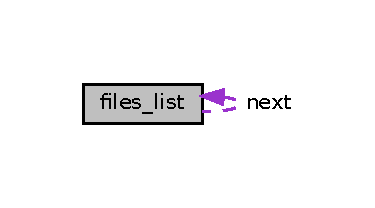
\includegraphics[width=180pt]{structfiles__list__coll__graph}
\end{center}
\end{figure}
\subsection*{Campi}
\begin{DoxyCompactItemize}
\item 
\mbox{\Hypertarget{structfiles__list_a986ecc1174faf39b15c1ef655c2ed966}\label{structfiles__list_a986ecc1174faf39b15c1ef655c2ed966}} 
char $\ast$ \hyperlink{structfiles__list_a986ecc1174faf39b15c1ef655c2ed966}{path}
\begin{DoxyCompactList}\small\item\em Percorso file. \end{DoxyCompactList}\item 
\mbox{\Hypertarget{structfiles__list_a3cdd0098b7fb9589480f8a9facad90ce}\label{structfiles__list_a3cdd0098b7fb9589480f8a9facad90ce}} 
struct \hyperlink{structfiles__list}{files\+\_\+list} $\ast$ \hyperlink{structfiles__list_a3cdd0098b7fb9589480f8a9facad90ce}{next}
\begin{DoxyCompactList}\small\item\em Puntatore al prossimo nodo. \end{DoxyCompactList}\end{DoxyCompactItemize}


\subsection{Descrizione dettagliata}
Nodo di una lista concatenata di file\+Path. 

La documentazione per questa struct è stata generata a partire dal seguente file\+:\begin{DoxyCompactItemize}
\item 
/mnt/c/\+Users/stefa/\+Desktop/progetti/system\+\_\+call/src/\hyperlink{files_8h}{files.\+h}\end{DoxyCompactItemize}

\hypertarget{unionsemun}{}\section{Riferimenti per la union semun}
\label{unionsemun}\index{semun@{semun}}


{\ttfamily \#include $<$common.\+h$>$}

\subsection*{Campi}
\begin{DoxyCompactItemize}
\item 
int \hyperlink{unionsemun_ac6121ecb6d04a024e07e12bd71b94031}{val}
\item 
struct semid\+\_\+ds $\ast$ \hyperlink{unionsemun_abe0ba6ad77214cee618027739e992503}{buf}
\item 
unsigned short $\ast$ \hyperlink{unionsemun_a1c74eb9326763d3854dc90167e1f4460}{array}
\end{DoxyCompactItemize}


\subsection{Descrizione dettagliata}
Union usata dalla system call semctl(). 

\subsection{Documentazione dei campi}
\mbox{\Hypertarget{unionsemun_a1c74eb9326763d3854dc90167e1f4460}\label{unionsemun_a1c74eb9326763d3854dc90167e1f4460}} 
\index{semun@{semun}!array@{array}}
\index{array@{array}!semun@{semun}}
\subsubsection{\texorpdfstring{array}{array}}
{\footnotesize\ttfamily unsigned short $\ast$ semun\+::array}

per eseguire operazioni su tutti i semafori. Usato dalle operazioni G\+E\+T\+A\+LL e S\+E\+T\+A\+LL \mbox{\Hypertarget{unionsemun_abe0ba6ad77214cee618027739e992503}\label{unionsemun_abe0ba6ad77214cee618027739e992503}} 
\index{semun@{semun}!buf@{buf}}
\index{buf@{buf}!semun@{semun}}
\subsubsection{\texorpdfstring{buf}{buf}}
{\footnotesize\ttfamily struct semid\+\_\+ds $\ast$ semun\+::buf}

usato per lavorare sullo stato globale del semaforo. Usato dalle operazioni I\+P\+C\+\_\+\+S\+T\+AT e I\+P\+C\+\_\+\+S\+ET \mbox{\Hypertarget{unionsemun_ac6121ecb6d04a024e07e12bd71b94031}\label{unionsemun_ac6121ecb6d04a024e07e12bd71b94031}} 
\index{semun@{semun}!val@{val}}
\index{val@{val}!semun@{semun}}
\subsubsection{\texorpdfstring{val}{val}}
{\footnotesize\ttfamily int semun\+::val}

usato se si lavora su un singolo semaforo. Usato dalla operazione S\+E\+T\+V\+AL 

La documentazione per questa union è stata generata a partire dai seguenti file\+:\begin{DoxyCompactItemize}
\item 
theory/semaphores/common.\+c\item 
theory/shared\+\_\+memory/common.\+h\item 
/mnt/c/\+Users/stefa/\+Desktop/new/system\+\_\+call/src/\hyperlink{semaphore_8h}{semaphore.\+h}\end{DoxyCompactItemize}

\chapter{Documentazione dei file}
\hypertarget{client_8c}{}\section{Riferimenti per il file /mnt/c/\+Users/stefa/\+Desktop/system\+\_\+call/src/client.c}
\label{client_8c}\index{/mnt/c/\+Users/stefa/\+Desktop/system\+\_\+call/src/client.\+c@{/mnt/c/\+Users/stefa/\+Desktop/system\+\_\+call/src/client.\+c}}


Contiene l\textquotesingle{}implementazione del client.  


{\ttfamily \#include $<$stdio.\+h$>$}\newline
{\ttfamily \#include $<$stdbool.\+h$>$}\newline
{\ttfamily \#include $<$unistd.\+h$>$}\newline
{\ttfamily \#include $<$signal.\+h$>$}\newline
{\ttfamily \#include $<$dirent.\+h$>$}\newline
{\ttfamily \#include $<$errno.\+h$>$}\newline
{\ttfamily \#include $<$stdlib.\+h$>$}\newline
{\ttfamily \#include $<$string.\+h$>$}\newline
{\ttfamily \#include $<$fcntl.\+h$>$}\newline
{\ttfamily \#include $<$sys/stat.\+h$>$}\newline
{\ttfamily \#include $<$sys/wait.\+h$>$}\newline
{\ttfamily \#include $<$sys/msg.\+h$>$}\newline
{\ttfamily \#include \char`\"{}defines.\+h\char`\"{}}\newline
{\ttfamily \#include \char`\"{}err\+\_\+exit.\+h\char`\"{}}\newline
{\ttfamily \#include \char`\"{}signals.\+h\char`\"{}}\newline
{\ttfamily \#include \char`\"{}files.\+h\char`\"{}}\newline
{\ttfamily \#include \char`\"{}client.\+h\char`\"{}}\newline
{\ttfamily \#include \char`\"{}semaphore.\+h\char`\"{}}\newline
{\ttfamily \#include \char`\"{}shared\+\_\+memory.\+h\char`\"{}}\newline
{\ttfamily \#include \char`\"{}fifo.\+h\char`\"{}}\newline
{\ttfamily \#include \char`\"{}debug.\+h\char`\"{}}\newline
Grafo delle dipendenze di inclusione per client.\+c\+:\nopagebreak
\begin{figure}[H]
\begin{center}
\leavevmode
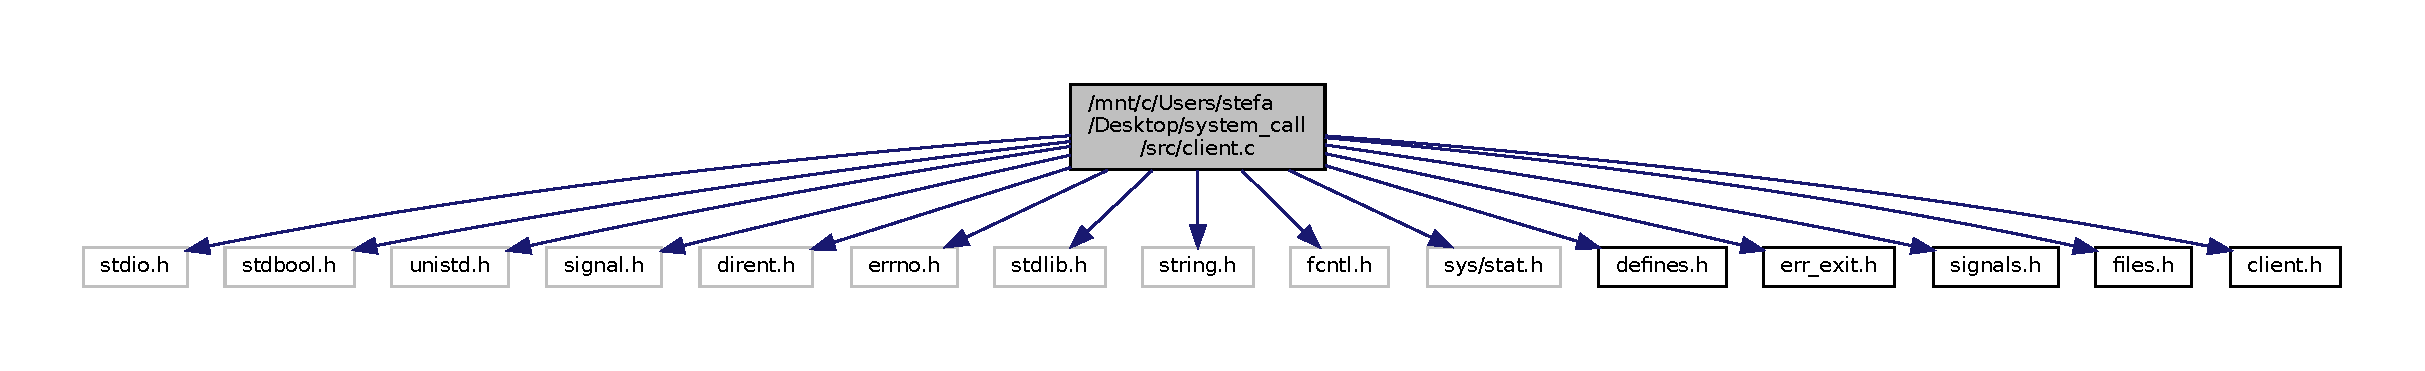
\includegraphics[width=350pt]{client_8c__incl}
\end{center}
\end{figure}
\subsection*{Funzioni}
\begin{DoxyCompactItemize}
\item 
char $\ast$ \hyperlink{client_8c_a748983b7ce27515a3ad116ada4334c4e}{int\+\_\+to\+\_\+string} (int value)
\item 
bool \hyperlink{client_8c_ac129a55ffa08a55addb9ea1afbd709f8}{str\+Equals} (char $\ast$a, char $\ast$b)
\item 
void \hyperlink{client_8c_a48d605ff689f470746c858648f0a98c2}{S\+I\+G\+I\+N\+T\+Signal\+Handler} (int sig)
\begin{DoxyCompactList}\small\item\em Chiude tutte le I\+PC e termina. \end{DoxyCompactList}\item 
void \hyperlink{client_8c_a8c7084a254c7cd640d66e647795ff8f6}{operazioni\+\_\+client0} ()
\item 
void \hyperlink{client_8c_a50b22adcb76198fcd9402a97ff4711bf}{S\+I\+G\+U\+S\+R1\+Signal\+Handler} (int sig)
\begin{DoxyCompactList}\small\item\em Handler del segnale S\+I\+G\+U\+S\+R1\+: chiude le risorse del client 0 e termina la sua esecuzione. \end{DoxyCompactList}\item 
void \hyperlink{client_8c_a55586f2b7e9b3620294cf78cda8abdad}{dividi} (int fd, char $\ast$buf, size\+\_\+t count, char $\ast$file\+Path, int parte)
\begin{DoxyCompactList}\small\item\em Divide in 4 parti il contenuto del file da inviare al server. \end{DoxyCompactList}\item 
void \hyperlink{client_8c_a54b47b58f228d7bc9827d2919687e25a}{operazioni\+\_\+figlio} (char $\ast$file\+Path)
\begin{DoxyCompactList}\small\item\em Funzione eseguita da ogni Client i (figli di Client 0) per mandare i file al server. \end{DoxyCompactList}\item 
int \hyperlink{client_8c_a0ddf1224851353fc92bfbff6f499fa97}{main} (int argc, char $\ast$argv\mbox{[}$\,$\mbox{]})
\end{DoxyCompactItemize}
\subsection*{Variabili}
\begin{DoxyCompactItemize}
\item 
\mbox{\Hypertarget{client_8c_a0e51f6e74ef591eef5a08e4a5a2d5ea8}\label{client_8c_a0e51f6e74ef591eef5a08e4a5a2d5ea8}} 
int \hyperlink{client_8c_a0e51f6e74ef591eef5a08e4a5a2d5ea8}{fifo1\+\_\+fd} = -\/1
\begin{DoxyCompactList}\small\item\em file descriptor prima fifo \end{DoxyCompactList}\item 
\mbox{\Hypertarget{client_8c_a4a1b7b9ae118e79117db0755b4588077}\label{client_8c_a4a1b7b9ae118e79117db0755b4588077}} 
int \hyperlink{client_8c_a4a1b7b9ae118e79117db0755b4588077}{fifo2\+\_\+fd} = -\/1
\begin{DoxyCompactList}\small\item\em file descriptor seconda fifo \end{DoxyCompactList}\item 
\mbox{\Hypertarget{client_8c_ae73e6a837794db6e63f23db2d64a8130}\label{client_8c_ae73e6a837794db6e63f23db2d64a8130}} 
int \hyperlink{client_8c_ae73e6a837794db6e63f23db2d64a8130}{msqid} = -\/1
\begin{DoxyCompactList}\small\item\em id coda dei messaggi \end{DoxyCompactList}\item 
\mbox{\Hypertarget{client_8c_a7c35ac5305085cf7360645b8d52988b5}\label{client_8c_a7c35ac5305085cf7360645b8d52988b5}} 
int \hyperlink{client_8c_a7c35ac5305085cf7360645b8d52988b5}{semid} = -\/1
\begin{DoxyCompactList}\small\item\em id set di semafori \end{DoxyCompactList}\item 
\mbox{\Hypertarget{client_8c_ac8807d215d2ee6d9779d76aeb1147430}\label{client_8c_ac8807d215d2ee6d9779d76aeb1147430}} 
int \hyperlink{client_8c_ac8807d215d2ee6d9779d76aeb1147430}{shmid} = -\/1
\begin{DoxyCompactList}\small\item\em id memoria condivisa messaggi \end{DoxyCompactList}\item 
\mbox{\Hypertarget{client_8c_a0b268ec51e0860874f687d0d1ffcd0e2}\label{client_8c_a0b268ec51e0860874f687d0d1ffcd0e2}} 
\hyperlink{structmsg__t}{msg\+\_\+t} $\ast$ \hyperlink{client_8c_a0b268ec51e0860874f687d0d1ffcd0e2}{shm\+\_\+ptr} = N\+U\+LL
\begin{DoxyCompactList}\small\item\em puntatore memoria condivisa messaggi \end{DoxyCompactList}\item 
\mbox{\Hypertarget{client_8c_aef99f0b2f4ff9b59d2e02bf8e9349d04}\label{client_8c_aef99f0b2f4ff9b59d2e02bf8e9349d04}} 
int \hyperlink{client_8c_aef99f0b2f4ff9b59d2e02bf8e9349d04}{shm\+\_\+check\+\_\+id} = -\/1
\begin{DoxyCompactList}\small\item\em id memoria condivisa flag lettura/scrittura messaggi \end{DoxyCompactList}\item 
\mbox{\Hypertarget{client_8c_a687e40faeef71a19cdd81e1bb787ca77}\label{client_8c_a687e40faeef71a19cdd81e1bb787ca77}} 
int $\ast$ \hyperlink{client_8c_a687e40faeef71a19cdd81e1bb787ca77}{shm\+\_\+check\+\_\+ptr} = N\+U\+LL
\begin{DoxyCompactList}\small\item\em puntatore memoria condivisa flag lettura/scrittura messaggi \end{DoxyCompactList}\item 
\mbox{\Hypertarget{client_8c_a709c4fcdc1217a8f8785cb59e85beee5}\label{client_8c_a709c4fcdc1217a8f8785cb59e85beee5}} 
char \hyperlink{client_8c_a709c4fcdc1217a8f8785cb59e85beee5}{E\+X\+E\+C\+U\+T\+A\+B\+L\+E\+\_\+\+D\+IR} \mbox{[}\hyperlink{defines_8h_a22ad48d95fdd6689ea92e17ca5bbfccb}{B\+U\+F\+F\+E\+R\+\_\+\+SZ}\mbox{]} = \char`\"{}\char`\"{}
\begin{DoxyCompactList}\small\item\em Percorso cartella eseguibile. \end{DoxyCompactList}\item 
\mbox{\Hypertarget{client_8c_ab68195a262278b18e5dc84f677ad434d}\label{client_8c_ab68195a262278b18e5dc84f677ad434d}} 
char $\ast$ \hyperlink{client_8c_ab68195a262278b18e5dc84f677ad434d}{search\+Path} = N\+U\+LL
\begin{DoxyCompactList}\small\item\em contiene percorso passato come parametro \end{DoxyCompactList}\end{DoxyCompactItemize}


\subsection{Descrizione dettagliata}
Contiene l\textquotesingle{}implementazione del client. 

\begin{DoxyRefDesc}{Da fare}
\item[\hyperlink{todo__todo000001}{Da fare}]Spostare le funzioni non main fuori dal file \hyperlink{client_8c}{client.\+c} ? (ad esempio una opzione per la funzione \hyperlink{client_8c_a55586f2b7e9b3620294cf78cda8abdad}{dividi()} e\textquotesingle{} metterla in \hyperlink{files_8c}{files.\+c}) \end{DoxyRefDesc}


\subsection{Documentazione delle funzioni}
\mbox{\Hypertarget{client_8c_a55586f2b7e9b3620294cf78cda8abdad}\label{client_8c_a55586f2b7e9b3620294cf78cda8abdad}} 
\index{client.\+c@{client.\+c}!dividi@{dividi}}
\index{dividi@{dividi}!client.\+c@{client.\+c}}
\subsubsection{\texorpdfstring{dividi()}{dividi()}}
{\footnotesize\ttfamily void dividi (\begin{DoxyParamCaption}\item[{int}]{fd,  }\item[{char $\ast$}]{buf,  }\item[{size\+\_\+t}]{count,  }\item[{char $\ast$}]{file\+Path,  }\item[{int}]{parte }\end{DoxyParamCaption})}



Divide in 4 parti il contenuto del file da inviare al server. 


\begin{DoxyParams}{Parametri}
{\em fd} & File descriptor del file da inviare \\
\hline
{\em buf} & Buffer in cui memorizzare la porzione del messaggio \\
\hline
{\em count} & Dimensione della porzione di messaggio \\
\hline
{\em file\+Path} & Percorso del file da suddividere \\
\hline
{\em parte} & Numero identificativo della porzione di messaggio \\
\hline
\end{DoxyParams}
Questo è il grafo dei chiamanti di questa funzione\+:\nopagebreak
\begin{figure}[H]
\begin{center}
\leavevmode
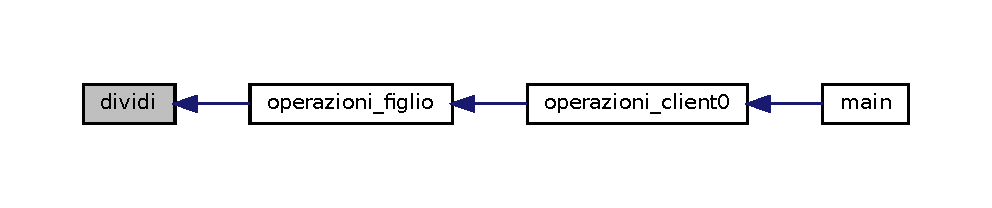
\includegraphics[width=350pt]{client_8c_a55586f2b7e9b3620294cf78cda8abdad_icgraph}
\end{center}
\end{figure}
\mbox{\Hypertarget{client_8c_a748983b7ce27515a3ad116ada4334c4e}\label{client_8c_a748983b7ce27515a3ad116ada4334c4e}} 
\index{client.\+c@{client.\+c}!int\+\_\+to\+\_\+string@{int\+\_\+to\+\_\+string}}
\index{int\+\_\+to\+\_\+string@{int\+\_\+to\+\_\+string}!client.\+c@{client.\+c}}
\subsubsection{\texorpdfstring{int\+\_\+to\+\_\+string()}{int\_to\_string()}}
{\footnotesize\ttfamily char$\ast$ int\+\_\+to\+\_\+string (\begin{DoxyParamCaption}\item[{int}]{value }\end{DoxyParamCaption})}

Converte un intero in stringa. \begin{quote}
E\textquotesingle{} necessaria la free() dopo aver terminato l\textquotesingle{}uso della stringa. \end{quote}



\begin{DoxyParams}{Parametri}
{\em value} & Valore intero da convertire in stringa \\
\hline
\end{DoxyParams}
\begin{DoxyReturn}{Restituisce}
char$\ast$ Stringa contenente il valore 
\end{DoxyReturn}
Questo è il grafo dei chiamanti di questa funzione\+:\nopagebreak
\begin{figure}[H]
\begin{center}
\leavevmode
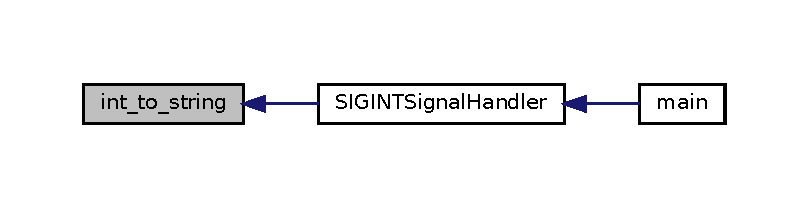
\includegraphics[width=350pt]{client_8c_a748983b7ce27515a3ad116ada4334c4e_icgraph}
\end{center}
\end{figure}
\mbox{\Hypertarget{client_8c_a0ddf1224851353fc92bfbff6f499fa97}\label{client_8c_a0ddf1224851353fc92bfbff6f499fa97}} 
\index{client.\+c@{client.\+c}!main@{main}}
\index{main@{main}!client.\+c@{client.\+c}}
\subsubsection{\texorpdfstring{main()}{main()}}
{\footnotesize\ttfamily int main (\begin{DoxyParamCaption}\item[{int}]{argc,  }\item[{char $\ast$}]{argv\mbox{[}$\,$\mbox{]} }\end{DoxyParamCaption})}

Memorizza il percorso passato come parametro, gestisce segnali e handler, attende i segnali S\+I\+G\+I\+NT o S\+I\+G\+U\+S\+R1.


\begin{DoxyParams}{Parametri}
{\em argc} & Numero argomenti passati da linea di comando (compreso il nome dell\textquotesingle{}eseguibile) \\
\hline
{\em argv} & Array di argomenti passati da linea di comando \\
\hline
\end{DoxyParams}
\begin{DoxyReturn}{Restituisce}
int Exit code dell\textquotesingle{}intero programma 
\end{DoxyReturn}
Questo è il grafo delle chiamate per questa funzione\+:
\nopagebreak
\begin{figure}[H]
\begin{center}
\leavevmode
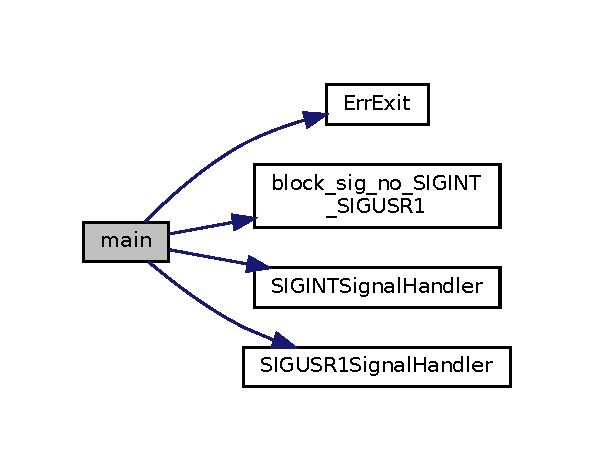
\includegraphics[width=350pt]{client_8c_a0ddf1224851353fc92bfbff6f499fa97_cgraph}
\end{center}
\end{figure}
\mbox{\Hypertarget{client_8c_a8c7084a254c7cd640d66e647795ff8f6}\label{client_8c_a8c7084a254c7cd640d66e647795ff8f6}} 
\index{client.\+c@{client.\+c}!operazioni\+\_\+client0@{operazioni\+\_\+client0}}
\index{operazioni\+\_\+client0@{operazioni\+\_\+client0}!client.\+c@{client.\+c}}
\subsubsection{\texorpdfstring{operazioni\+\_\+client0()}{operazioni\_client0()}}
{\footnotesize\ttfamily void operazioni\+\_\+client0 (\begin{DoxyParamCaption}{ }\end{DoxyParamCaption})}

Esegue tutte le funzionalita\textquotesingle{} principali del client 0.

Non vengono eseguite in \hyperlink{client_8h_a48d605ff689f470746c858648f0a98c2}{S\+I\+G\+I\+N\+T\+Signal\+Handler()} per il seguente motivo\+: \href{https://man7.org/linux/man-pages/man7/signal-safety.7.html}{\tt https\+://man7.\+org/linux/man-\/pages/man7/signal-\/safety.\+7.\+html}

\begin{DoxyRefDesc}{Da fare}
\item[\hyperlink{todo__todo000002}{Da fare}]Potrebbe essere necessario ottimizzare l\textquotesingle{}uso dello H\+E\+AP nel client 0. Attualmente la dimensione massima occupata dal client e\textquotesingle{}\+: \$\$100 file $\ast$ dim. path + 100 file $\ast$ dim. pointer\$\$. Assumento dim. path massima = 250 caratteri e dim. pointer 4 byte (32 bit)\+: \$\$100 $\ast$ 250 + 100 $\ast$ 4 = 25400\$\$ Quindi solo lato client si occupano 25 K\+Byte. Quando viene creato un client esso eredita momentaneamente la lista creando al massimo un\textquotesingle{}altra lista concatenata. Quindi in pratica si occupano\+: \$\$25 $\ast$ 2 = 50\$\$ Ovvero 50 KB.\end{DoxyRefDesc}


\begin{DoxyRefDesc}{Warnings}
\item[\hyperlink{warning__warning000001}{Warnings}]Per ottimizzare l\textquotesingle{}uso dello H\+E\+AP nel client 0 si potrebbe prima cercare e contare quanti file sono presenti senza creare una lista concatenata e poi ricercare i file e man mano che si trovano file send\+\_\+me si puo\textquotesingle{} creare il processo figlio per inviare il file. Per fare questo B\+I\+S\+O\+G\+NA sapere se il numero di file puo\textquotesingle{} cambiare durante l\textquotesingle{}esecuzione di questa funzione\+: se trovo 3 file e dopo un file viene cancellato cosa succede? ~\newline
 N\+O\+TA\+: questo problema puo\textquotesingle{} esserci anche nella situazione attuale...\end{DoxyRefDesc}


\begin{DoxyRefDesc}{Warnings}
\item[\hyperlink{warning__warning000002}{Warnings}]Il client 0 deve attendere i processi figlio? La specifica indica solo che bisogna attendere il messaggio di fine dal server... Attualmente prima si attendere il messaggio di fine e poi si aspetta che tutti i figlio terminino.\end{DoxyRefDesc}


\begin{DoxyRefDesc}{Warnings}
\item[\hyperlink{warning__warning000003}{Warnings}]Il percorso passato al client deve essere assoluto o puo\textquotesingle{} essere relativo? Se si passa un percorso relativo chdir() fallira\textquotesingle{} alla seconda esecuzione. ~\newline
 S\+O\+L\+U\+Z\+I\+O\+NE\+: si potrebbe usare un altro chdir() a fine funzione per tornare al percorso di esecuzione iniziale anticipando il chdir() successivo.\end{DoxyRefDesc}
Questo è il grafo delle chiamate per questa funzione\+:\nopagebreak
\begin{figure}[H]
\begin{center}
\leavevmode
\includegraphics[width=350pt]{client_8c_a8c7084a254c7cd640d66e647795ff8f6_cgraph}
\end{center}
\end{figure}
Questo è il grafo dei chiamanti di questa funzione\+:\nopagebreak
\begin{figure}[H]
\begin{center}
\leavevmode
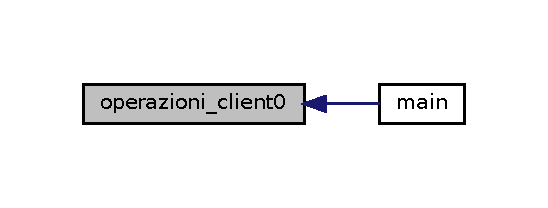
\includegraphics[width=263pt]{client_8c_a8c7084a254c7cd640d66e647795ff8f6_icgraph}
\end{center}
\end{figure}
\mbox{\Hypertarget{client_8c_a54b47b58f228d7bc9827d2919687e25a}\label{client_8c_a54b47b58f228d7bc9827d2919687e25a}} 
\index{client.\+c@{client.\+c}!operazioni\+\_\+figlio@{operazioni\+\_\+figlio}}
\index{operazioni\+\_\+figlio@{operazioni\+\_\+figlio}!client.\+c@{client.\+c}}
\subsubsection{\texorpdfstring{operazioni\+\_\+figlio()}{operazioni\_figlio()}}
{\footnotesize\ttfamily void operazioni\+\_\+figlio (\begin{DoxyParamCaption}\item[{char $\ast$}]{file\+Path }\end{DoxyParamCaption})}



Funzione eseguita da ogni Client i (figli di Client 0) per mandare i file al server. 


\begin{DoxyParams}{Parametri}
{\em file\+Path} & Percorso del file che il client deve suddividere e mandare al server. \\
\hline
\end{DoxyParams}
Questo è il grafo delle chiamate per questa funzione\+:\nopagebreak
\begin{figure}[H]
\begin{center}
\leavevmode
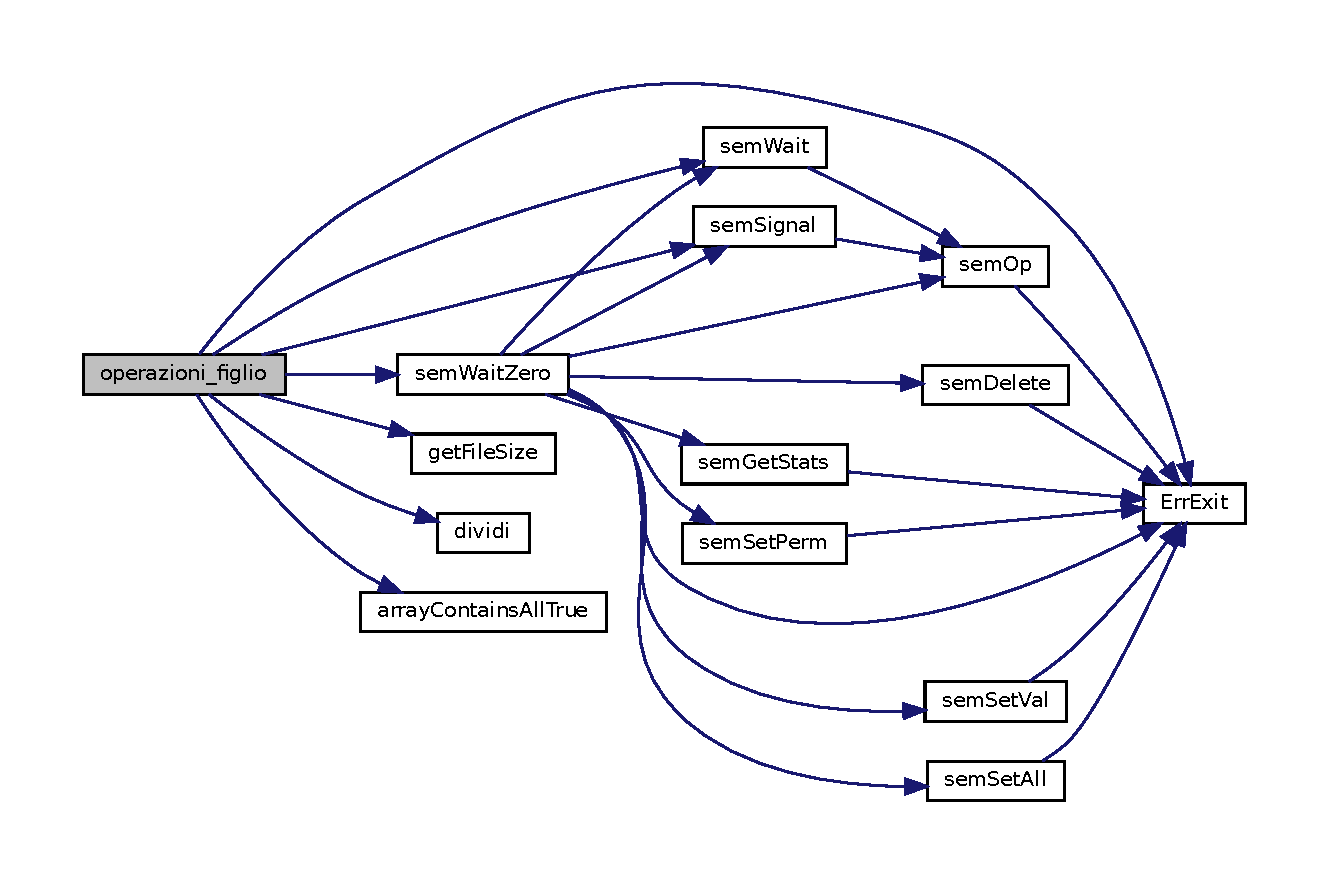
\includegraphics[width=350pt]{client_8c_a54b47b58f228d7bc9827d2919687e25a_cgraph}
\end{center}
\end{figure}
Questo è il grafo dei chiamanti di questa funzione\+:\nopagebreak
\begin{figure}[H]
\begin{center}
\leavevmode
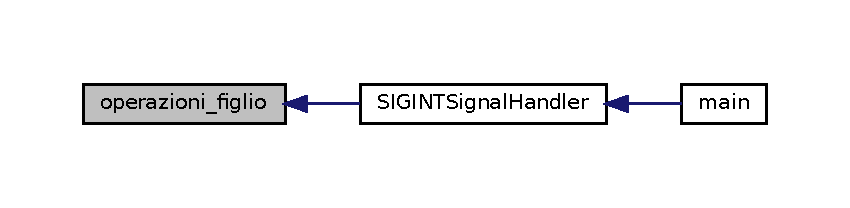
\includegraphics[width=350pt]{client_8c_a54b47b58f228d7bc9827d2919687e25a_icgraph}
\end{center}
\end{figure}
\mbox{\Hypertarget{client_8c_a48d605ff689f470746c858648f0a98c2}\label{client_8c_a48d605ff689f470746c858648f0a98c2}} 
\index{client.\+c@{client.\+c}!S\+I\+G\+I\+N\+T\+Signal\+Handler@{S\+I\+G\+I\+N\+T\+Signal\+Handler}}
\index{S\+I\+G\+I\+N\+T\+Signal\+Handler@{S\+I\+G\+I\+N\+T\+Signal\+Handler}!client.\+c@{client.\+c}}
\subsubsection{\texorpdfstring{S\+I\+G\+I\+N\+T\+Signal\+Handler()}{SIGINTSignalHandler()}}
{\footnotesize\ttfamily void S\+I\+G\+I\+N\+T\+Signal\+Handler (\begin{DoxyParamCaption}\item[{int}]{sig }\end{DoxyParamCaption})}



Chiude tutte le I\+PC e termina. 

Handler del segnale S\+I\+G\+I\+NT.

Non fa niente, permette solo al processo di risvegliarsi dal pause().

Le funzionalita\textquotesingle{} principali vengono eseguite da \hyperlink{client_8h_a8c7084a254c7cd640d66e647795ff8f6}{operazioni\+\_\+client0()} e non qui per il seguente motivo\+: \href{https://man7.org/linux/man-pages/man7/signal-safety.7.html}{\tt https\+://man7.\+org/linux/man-\/pages/man7/signal-\/safety.\+7.\+html}


\begin{DoxyParams}{Parametri}
{\em sig} & Valore intero corrispondente a S\+I\+G\+I\+NT \\
\hline
\end{DoxyParams}
Questo è il grafo dei chiamanti di questa funzione\+:\nopagebreak
\begin{figure}[H]
\begin{center}
\leavevmode
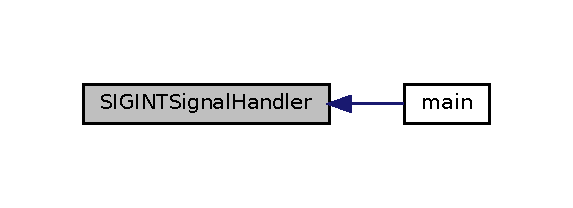
\includegraphics[width=275pt]{client_8c_a48d605ff689f470746c858648f0a98c2_icgraph}
\end{center}
\end{figure}
\mbox{\Hypertarget{client_8c_a50b22adcb76198fcd9402a97ff4711bf}\label{client_8c_a50b22adcb76198fcd9402a97ff4711bf}} 
\index{client.\+c@{client.\+c}!S\+I\+G\+U\+S\+R1\+Signal\+Handler@{S\+I\+G\+U\+S\+R1\+Signal\+Handler}}
\index{S\+I\+G\+U\+S\+R1\+Signal\+Handler@{S\+I\+G\+U\+S\+R1\+Signal\+Handler}!client.\+c@{client.\+c}}
\subsubsection{\texorpdfstring{S\+I\+G\+U\+S\+R1\+Signal\+Handler()}{SIGUSR1SignalHandler()}}
{\footnotesize\ttfamily void S\+I\+G\+U\+S\+R1\+Signal\+Handler (\begin{DoxyParamCaption}\item[{int}]{sig }\end{DoxyParamCaption})}



Handler del segnale S\+I\+G\+U\+S\+R1\+: chiude le risorse del client 0 e termina la sua esecuzione. 


\begin{DoxyParams}{Parametri}
{\em sig} & Valore intero corrispondente a S\+I\+G\+U\+S\+R1 \\
\hline
\end{DoxyParams}
Questo è il grafo delle chiamate per questa funzione\+:\nopagebreak
\begin{figure}[H]
\begin{center}
\leavevmode
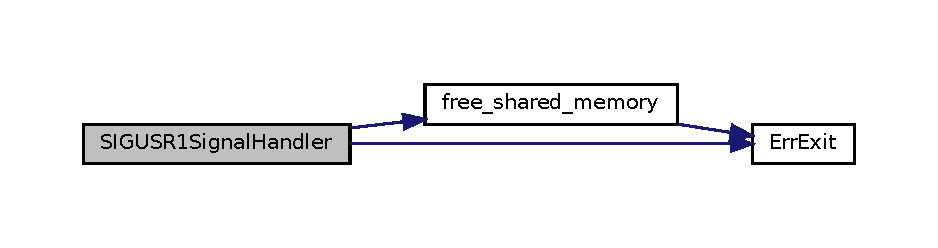
\includegraphics[width=350pt]{client_8c_a50b22adcb76198fcd9402a97ff4711bf_cgraph}
\end{center}
\end{figure}
Questo è il grafo dei chiamanti di questa funzione\+:\nopagebreak
\begin{figure}[H]
\begin{center}
\leavevmode
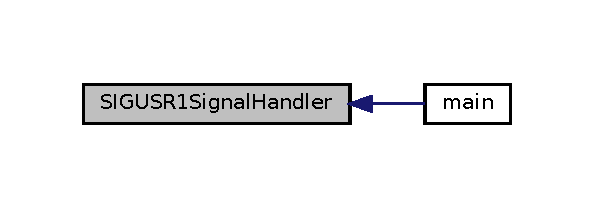
\includegraphics[width=285pt]{client_8c_a50b22adcb76198fcd9402a97ff4711bf_icgraph}
\end{center}
\end{figure}
\mbox{\Hypertarget{client_8c_ac129a55ffa08a55addb9ea1afbd709f8}\label{client_8c_ac129a55ffa08a55addb9ea1afbd709f8}} 
\index{client.\+c@{client.\+c}!str\+Equals@{str\+Equals}}
\index{str\+Equals@{str\+Equals}!client.\+c@{client.\+c}}
\subsubsection{\texorpdfstring{str\+Equals()}{strEquals()}}
{\footnotesize\ttfamily bool str\+Equals (\begin{DoxyParamCaption}\item[{char $\ast$}]{a,  }\item[{char $\ast$}]{b }\end{DoxyParamCaption})}

Restituisce vero se due stringhe sono uguali


\begin{DoxyParams}{Parametri}
{\em a} & Stringa da confrontare \\
\hline
{\em b} & Stringa da confrontare \\
\hline
\end{DoxyParams}
\begin{DoxyReturn}{Restituisce}
true a e b sono uguali 

false a e b sono diverse 
\end{DoxyReturn}
Questo è il grafo dei chiamanti di questa funzione\+:\nopagebreak
\begin{figure}[H]
\begin{center}
\leavevmode
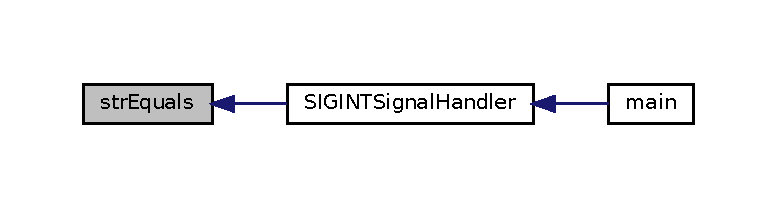
\includegraphics[width=350pt]{client_8c_ac129a55ffa08a55addb9ea1afbd709f8_icgraph}
\end{center}
\end{figure}

\hypertarget{client_8h}{}\section{Riferimenti per il file /mnt/c/\+Users/stefa/\+Desktop/system\+\_\+call/src/client.h}
\label{client_8h}\index{/mnt/c/\+Users/stefa/\+Desktop/system\+\_\+call/src/client.\+h@{/mnt/c/\+Users/stefa/\+Desktop/system\+\_\+call/src/client.\+h}}


Contiene la definizioni di variabili e funzioni specifiche del C\+L\+I\+E\+NT.  


Questo grafo mostra quali altri file includono direttamente o indirettamente questo file\+:\nopagebreak
\begin{figure}[H]
\begin{center}
\leavevmode
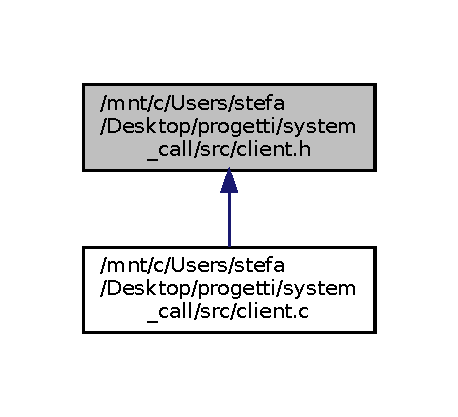
\includegraphics[width=202pt]{client_8h__dep__incl}
\end{center}
\end{figure}
\subsection*{Funzioni}
\begin{DoxyCompactItemize}
\item 
void \hyperlink{client_8h_a8c7084a254c7cd640d66e647795ff8f6}{operazioni\+\_\+client0} ()
\item 
void \hyperlink{client_8h_a48d605ff689f470746c858648f0a98c2}{S\+I\+G\+I\+N\+T\+Signal\+Handler} (int sig)
\begin{DoxyCompactList}\small\item\em Chiude tutte le I\+PC e termina. \end{DoxyCompactList}\item 
void \hyperlink{client_8h_a50b22adcb76198fcd9402a97ff4711bf}{S\+I\+G\+U\+S\+R1\+Signal\+Handler} (int sig)
\begin{DoxyCompactList}\small\item\em Handler del segnale S\+I\+G\+U\+S\+R1\+: chiude le risorse del client 0 e termina la sua esecuzione. \end{DoxyCompactList}\item 
void \hyperlink{client_8h_a55586f2b7e9b3620294cf78cda8abdad}{dividi} (int fd, char $\ast$buf, size\+\_\+t count, char $\ast$file\+Path, int parte)
\begin{DoxyCompactList}\small\item\em Divide in 4 parti il contenuto del file da inviare al server. \end{DoxyCompactList}\item 
void \hyperlink{client_8h_a54b47b58f228d7bc9827d2919687e25a}{operazioni\+\_\+figlio} (char $\ast$file\+Path)
\begin{DoxyCompactList}\small\item\em Funzione eseguita da ogni Client i (figli di Client 0) per mandare i file al server. \end{DoxyCompactList}\item 
int \hyperlink{client_8h_a0ddf1224851353fc92bfbff6f499fa97}{main} (int argc, char $\ast$argv\mbox{[}$\,$\mbox{]})
\item 
char $\ast$ \hyperlink{client_8h_a748983b7ce27515a3ad116ada4334c4e}{int\+\_\+to\+\_\+string} (int value)
\item 
bool \hyperlink{client_8h_ac129a55ffa08a55addb9ea1afbd709f8}{str\+Equals} (char $\ast$a, char $\ast$b)
\end{DoxyCompactItemize}


\subsection{Descrizione dettagliata}
Contiene la definizioni di variabili e funzioni specifiche del C\+L\+I\+E\+NT. 



\subsection{Documentazione delle funzioni}
\mbox{\Hypertarget{client_8h_a55586f2b7e9b3620294cf78cda8abdad}\label{client_8h_a55586f2b7e9b3620294cf78cda8abdad}} 
\index{client.\+h@{client.\+h}!dividi@{dividi}}
\index{dividi@{dividi}!client.\+h@{client.\+h}}
\subsubsection{\texorpdfstring{dividi()}{dividi()}}
{\footnotesize\ttfamily void dividi (\begin{DoxyParamCaption}\item[{int}]{fd,  }\item[{char $\ast$}]{buf,  }\item[{size\+\_\+t}]{count,  }\item[{char $\ast$}]{file\+Path,  }\item[{int}]{parte }\end{DoxyParamCaption})}



Divide in 4 parti il contenuto del file da inviare al server. 


\begin{DoxyParams}{Parametri}
{\em fd} & File descriptor del file da inviare \\
\hline
{\em buf} & Buffer in cui memorizzare la porzione del messaggio \\
\hline
{\em count} & Dimensione della porzione di messaggio \\
\hline
{\em file\+Path} & Percorso del file da suddividere \\
\hline
{\em parte} & Numero identificativo della porzione di messaggio \\
\hline
\end{DoxyParams}
Questo è il grafo dei chiamanti di questa funzione\+:\nopagebreak
\begin{figure}[H]
\begin{center}
\leavevmode
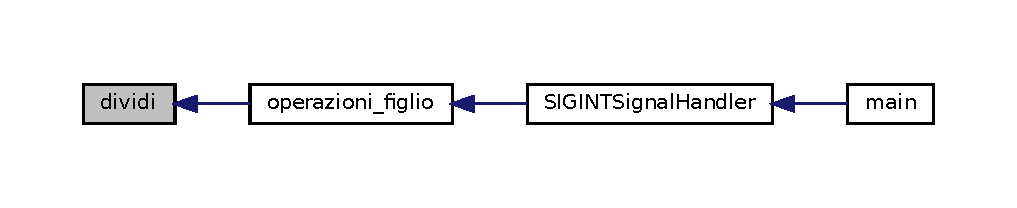
\includegraphics[width=350pt]{client_8h_a55586f2b7e9b3620294cf78cda8abdad_icgraph}
\end{center}
\end{figure}
\mbox{\Hypertarget{client_8h_a748983b7ce27515a3ad116ada4334c4e}\label{client_8h_a748983b7ce27515a3ad116ada4334c4e}} 
\index{client.\+h@{client.\+h}!int\+\_\+to\+\_\+string@{int\+\_\+to\+\_\+string}}
\index{int\+\_\+to\+\_\+string@{int\+\_\+to\+\_\+string}!client.\+h@{client.\+h}}
\subsubsection{\texorpdfstring{int\+\_\+to\+\_\+string()}{int\_to\_string()}}
{\footnotesize\ttfamily char$\ast$ int\+\_\+to\+\_\+string (\begin{DoxyParamCaption}\item[{int}]{value }\end{DoxyParamCaption})}

Converte un intero in stringa. \begin{quote}
E\textquotesingle{} necessaria la free() dopo aver terminato l\textquotesingle{}uso della stringa. \end{quote}



\begin{DoxyParams}{Parametri}
{\em value} & Valore intero da convertire in stringa \\
\hline
\end{DoxyParams}
\begin{DoxyReturn}{Restituisce}
char$\ast$ Stringa contenente il valore 
\end{DoxyReturn}
Questo è il grafo dei chiamanti di questa funzione\+:\nopagebreak
\begin{figure}[H]
\begin{center}
\leavevmode
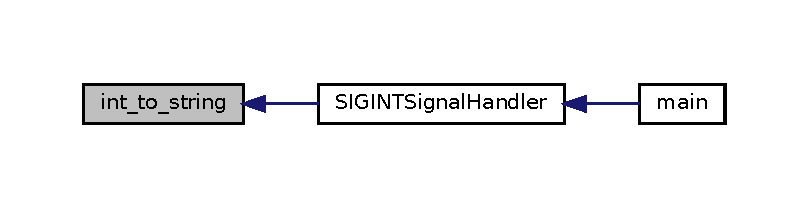
\includegraphics[width=350pt]{client_8h_a748983b7ce27515a3ad116ada4334c4e_icgraph}
\end{center}
\end{figure}
\mbox{\Hypertarget{client_8h_a0ddf1224851353fc92bfbff6f499fa97}\label{client_8h_a0ddf1224851353fc92bfbff6f499fa97}} 
\index{client.\+h@{client.\+h}!main@{main}}
\index{main@{main}!client.\+h@{client.\+h}}
\subsubsection{\texorpdfstring{main()}{main()}}
{\footnotesize\ttfamily int main (\begin{DoxyParamCaption}\item[{int}]{argc,  }\item[{char $\ast$}]{argv\mbox{[}$\,$\mbox{]} }\end{DoxyParamCaption})}

Memorizza il percorso passato come parametro, gestisce segnali e handler, attende i segnali S\+I\+G\+I\+NT o S\+I\+G\+U\+S\+R1.


\begin{DoxyParams}{Parametri}
{\em argc} & Numero argomenti passati da linea di comando (compreso il nome dell\textquotesingle{}eseguibile) \\
\hline
{\em argv} & Array di argomenti passati da linea di comando \\
\hline
\end{DoxyParams}
\begin{DoxyReturn}{Restituisce}
int Exit code dell\textquotesingle{}intero programma
\end{DoxyReturn}
Esegue operazioni principali del server.

terminazione effettuata con S\+I\+G\+I\+NT\+: Al termine chiudi tutte le I\+PC.

\begin{DoxyRefDesc}{Warnings}
\item[\hyperlink{warning__warning000004}{Warnings}]I file devono essere riuniti appena vengono ricevuti i 4 pezzi oppure va bene riunirli alla fine? \end{DoxyRefDesc}
Questo è il grafo delle chiamate per questa funzione\+:
\nopagebreak
\begin{figure}[H]
\begin{center}
\leavevmode
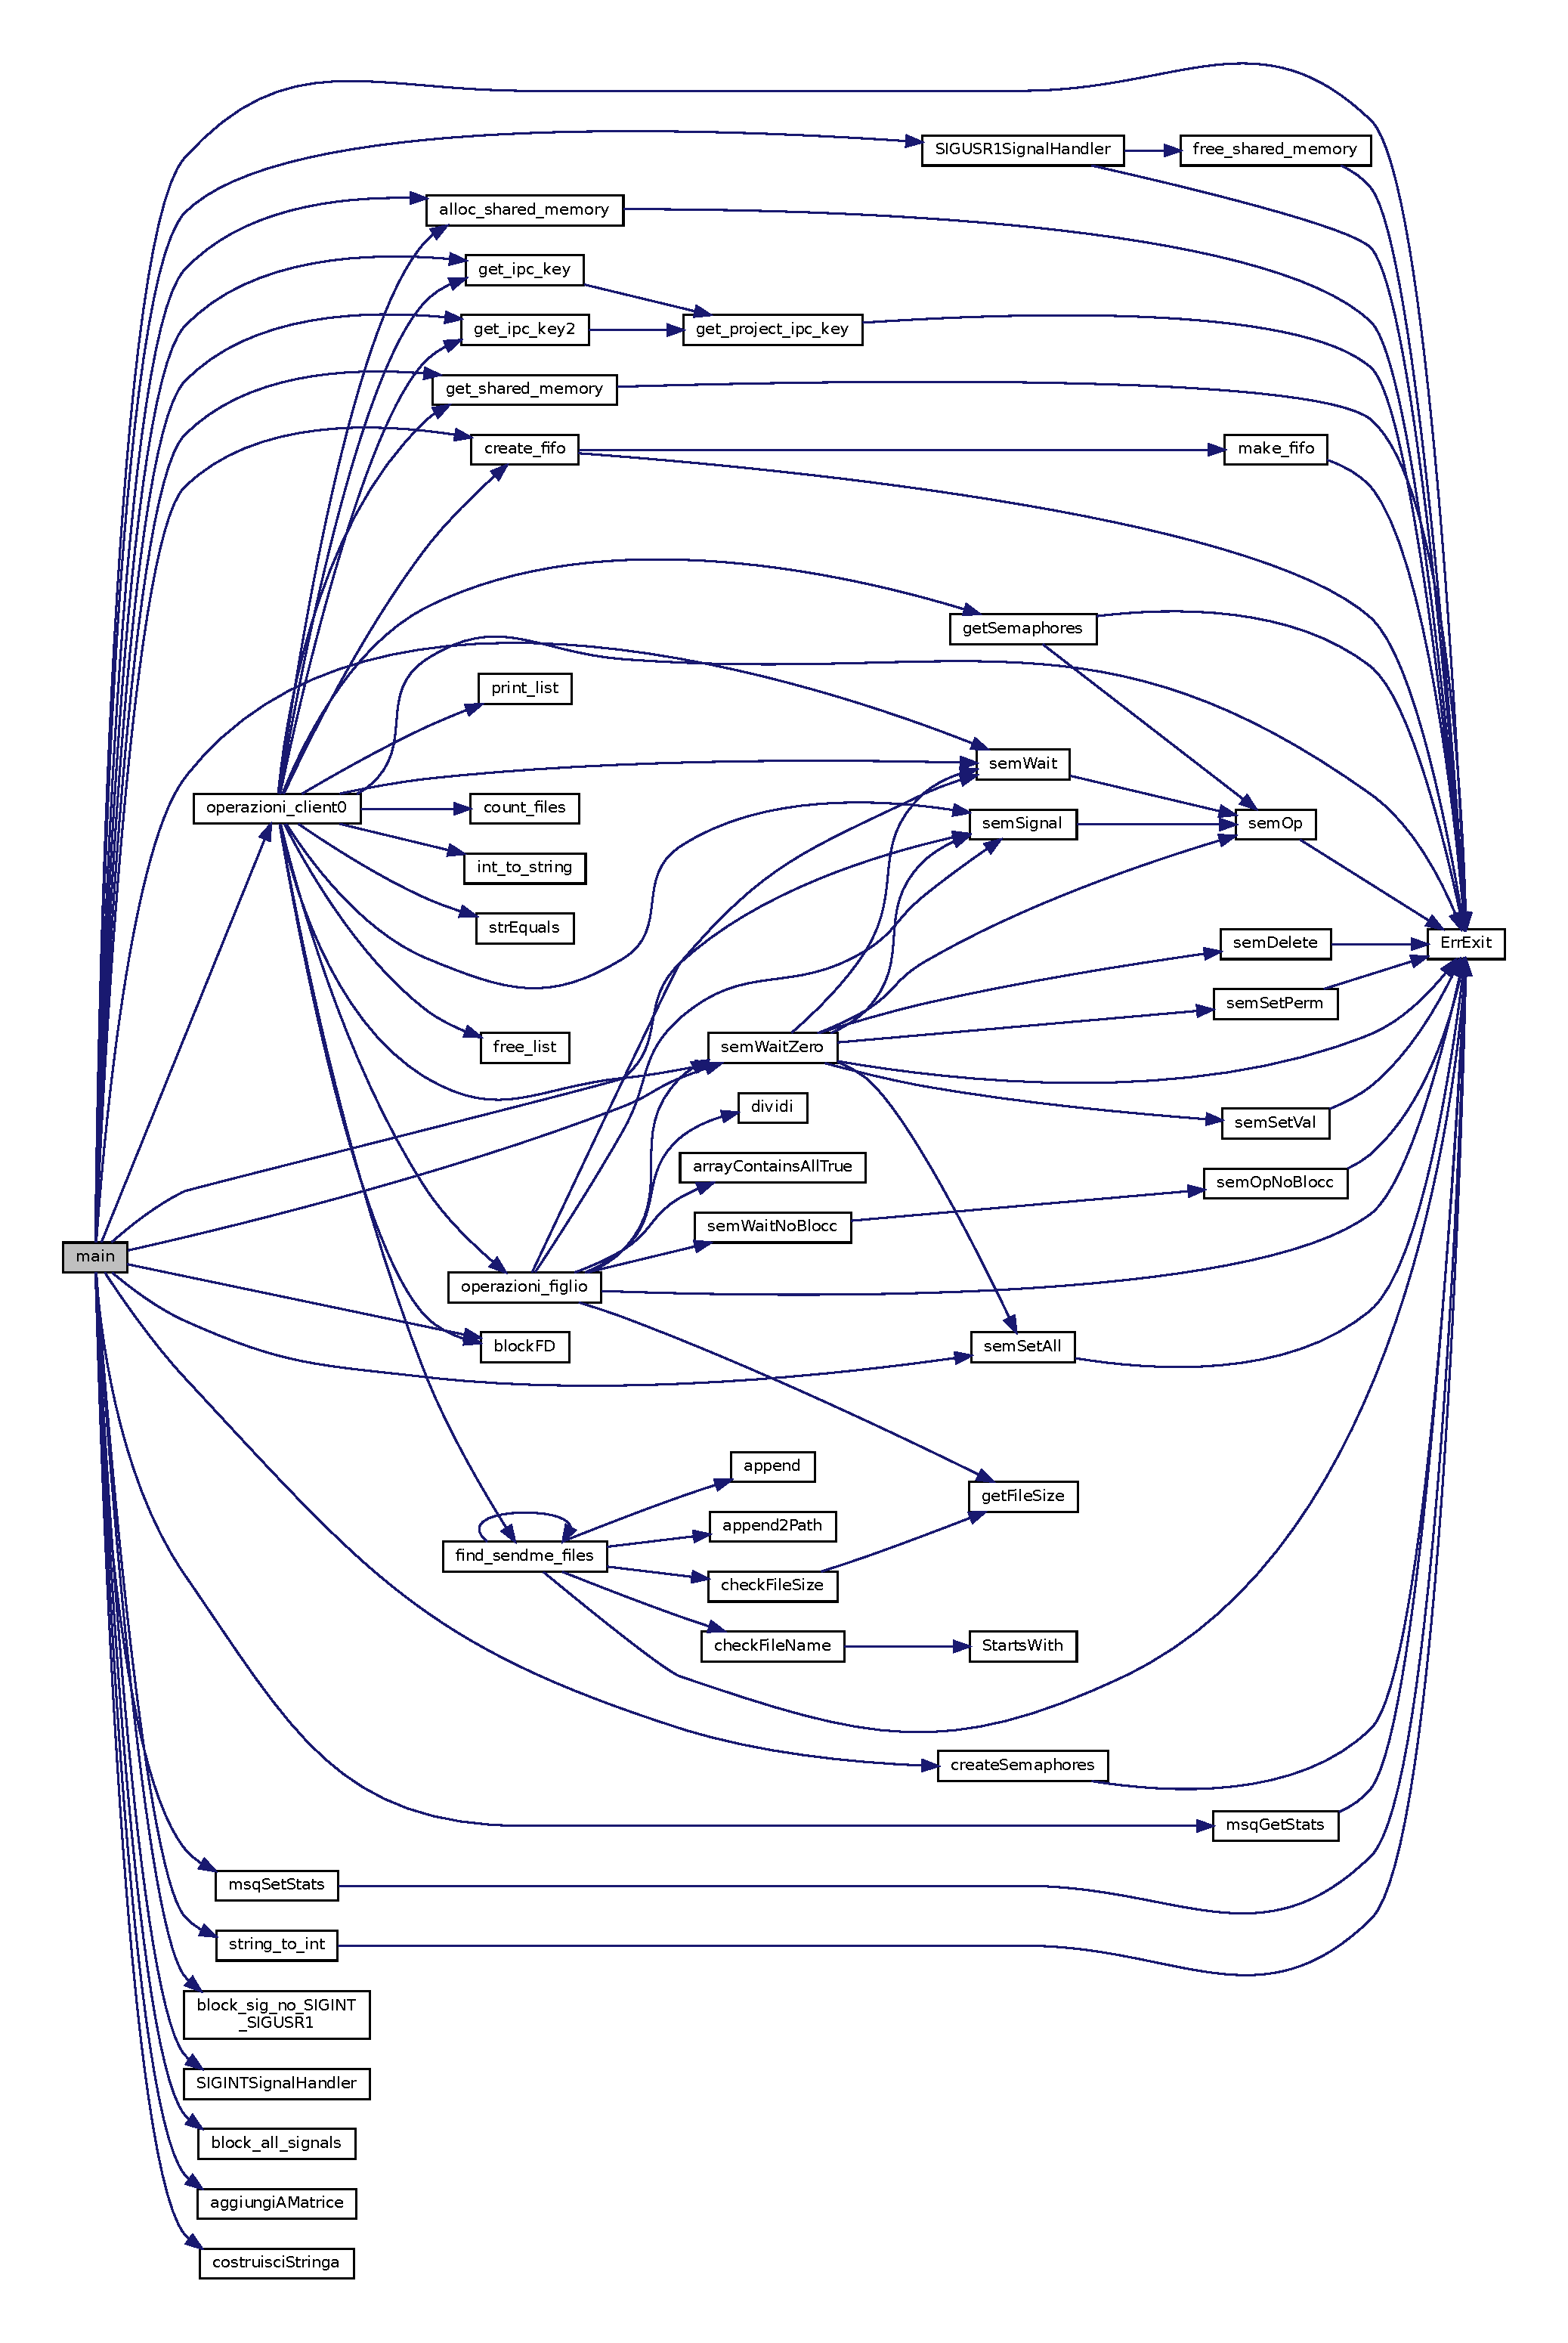
\includegraphics[width=350pt]{client_8h_a0ddf1224851353fc92bfbff6f499fa97_cgraph}
\end{center}
\end{figure}
\mbox{\Hypertarget{client_8h_a8c7084a254c7cd640d66e647795ff8f6}\label{client_8h_a8c7084a254c7cd640d66e647795ff8f6}} 
\index{client.\+h@{client.\+h}!operazioni\+\_\+client0@{operazioni\+\_\+client0}}
\index{operazioni\+\_\+client0@{operazioni\+\_\+client0}!client.\+h@{client.\+h}}
\subsubsection{\texorpdfstring{operazioni\+\_\+client0()}{operazioni\_client0()}}
{\footnotesize\ttfamily void operazioni\+\_\+client0 (\begin{DoxyParamCaption}{ }\end{DoxyParamCaption})}

Esegue tutte le funzionalita\textquotesingle{} principali del client 0.

Non vengono eseguite in \hyperlink{client_8h_a48d605ff689f470746c858648f0a98c2}{S\+I\+G\+I\+N\+T\+Signal\+Handler()} per il seguente motivo\+: \href{https://man7.org/linux/man-pages/man7/signal-safety.7.html}{\tt https\+://man7.\+org/linux/man-\/pages/man7/signal-\/safety.\+7.\+html}

\begin{DoxyRefDesc}{Da fare}
\item[\hyperlink{todo__todo000003}{Da fare}]Potrebbe essere necessario ottimizzare l\textquotesingle{}uso dello H\+E\+AP nel client 0. Attualmente la dimensione massima occupata dal client e\textquotesingle{}\+: \$\$100 file $\ast$ dim. path + 100 file $\ast$ dim. pointer\$\$. Assumento dim. path massima = 250 caratteri e dim. pointer 4 byte (32 bit)\+: \$\$100 $\ast$ 250 + 100 $\ast$ 4 = 25400\$\$ Quindi solo lato client si occupano 25 K\+Byte. Quando viene creato un client esso eredita momentaneamente la lista creando al massimo un\textquotesingle{}altra lista concatenata. Quindi in pratica si occupano\+: \$\$25 $\ast$ 2 = 50\$\$ Ovvero 50 KB.\end{DoxyRefDesc}


\begin{DoxyRefDesc}{Da fare}
\item[\hyperlink{todo__todo000004}{Da fare}]msgrcv e\textquotesingle{} bloccante quando flag = 0 e non ci sono messaggi da leggere quindi il while si potrebbe rimuovere.\end{DoxyRefDesc}


\begin{DoxyRefDesc}{Warnings}
\item[\hyperlink{warning__warning000001}{Warnings}]Per ottimizzare l\textquotesingle{}uso dello H\+E\+AP nel client 0 si potrebbe prima cercare e contare quanti file sono presenti senza creare una lista concatenata e poi ricercare i file e man mano che si trovano file send\+\_\+me si puo\textquotesingle{} creare il processo figlio per inviare il file. Per fare questo B\+I\+S\+O\+G\+NA sapere se il numero di file puo\textquotesingle{} cambiare durante l\textquotesingle{}esecuzione di questa funzione\+: se trovo 3 file e dopo un file viene cancellato cosa succede? ~\newline
 N\+O\+TA\+: questo problema puo\textquotesingle{} esserci anche nella situazione attuale...\end{DoxyRefDesc}


\begin{DoxyRefDesc}{Warnings}
\item[\hyperlink{warning__warning000002}{Warnings}]Il client 0 deve attendere i processi figlio? La specifica indica solo che bisogna attendere il messaggio di fine dal server... Attualmente prima si attendere il messaggio di fine e poi si aspetta che tutti i figlio terminino.\end{DoxyRefDesc}


\begin{DoxyRefDesc}{Warnings}
\item[\hyperlink{warning__warning000003}{Warnings}]Il percorso passato al client deve essere assoluto o puo\textquotesingle{} essere relativo? Se si passa un percorso relativo chdir() fallira\textquotesingle{} alla seconda esecuzione. ~\newline
 S\+O\+L\+U\+Z\+I\+O\+NE\+: si potrebbe usare un altro chdir() a fine funzione per tornare al percorso di esecuzione iniziale anticipando il chdir() successivo.\end{DoxyRefDesc}
Questo è il grafo delle chiamate per questa funzione\+:
\nopagebreak
\begin{figure}[H]
\begin{center}
\leavevmode
\includegraphics[width=350pt]{client_8h_a8c7084a254c7cd640d66e647795ff8f6_cgraph}
\end{center}
\end{figure}
Questo è il grafo dei chiamanti di questa funzione\+:
\nopagebreak
\begin{figure}[H]
\begin{center}
\leavevmode
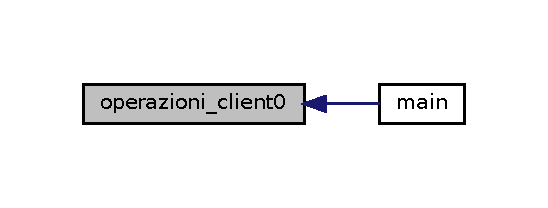
\includegraphics[width=263pt]{client_8h_a8c7084a254c7cd640d66e647795ff8f6_icgraph}
\end{center}
\end{figure}
\mbox{\Hypertarget{client_8h_a54b47b58f228d7bc9827d2919687e25a}\label{client_8h_a54b47b58f228d7bc9827d2919687e25a}} 
\index{client.\+h@{client.\+h}!operazioni\+\_\+figlio@{operazioni\+\_\+figlio}}
\index{operazioni\+\_\+figlio@{operazioni\+\_\+figlio}!client.\+h@{client.\+h}}
\subsubsection{\texorpdfstring{operazioni\+\_\+figlio()}{operazioni\_figlio()}}
{\footnotesize\ttfamily void operazioni\+\_\+figlio (\begin{DoxyParamCaption}\item[{char $\ast$}]{file\+Path }\end{DoxyParamCaption})}



Funzione eseguita da ogni Client i (figli di Client 0) per mandare i file al server. 


\begin{DoxyParams}{Parametri}
{\em file\+Path} & Percorso del file che il client deve suddividere e mandare al server. \\
\hline
\end{DoxyParams}
Questo è il grafo delle chiamate per questa funzione\+:
\nopagebreak
\begin{figure}[H]
\begin{center}
\leavevmode
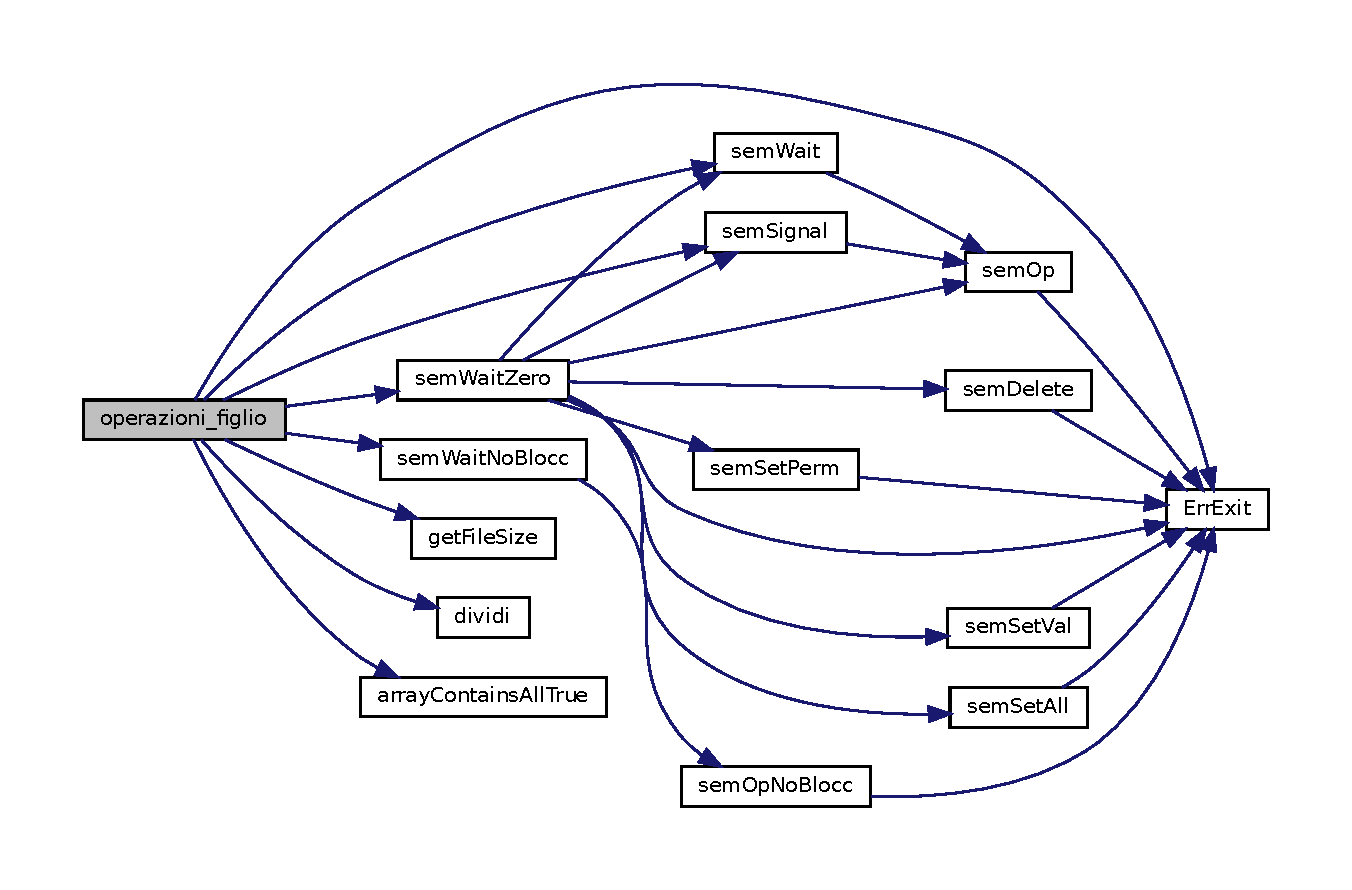
\includegraphics[width=350pt]{client_8h_a54b47b58f228d7bc9827d2919687e25a_cgraph}
\end{center}
\end{figure}
Questo è il grafo dei chiamanti di questa funzione\+:
\nopagebreak
\begin{figure}[H]
\begin{center}
\leavevmode
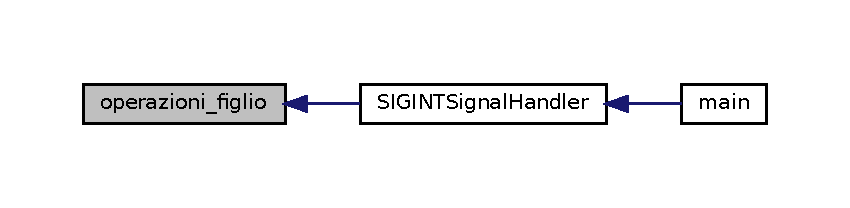
\includegraphics[width=350pt]{client_8h_a54b47b58f228d7bc9827d2919687e25a_icgraph}
\end{center}
\end{figure}
\mbox{\Hypertarget{client_8h_a48d605ff689f470746c858648f0a98c2}\label{client_8h_a48d605ff689f470746c858648f0a98c2}} 
\index{client.\+h@{client.\+h}!S\+I\+G\+I\+N\+T\+Signal\+Handler@{S\+I\+G\+I\+N\+T\+Signal\+Handler}}
\index{S\+I\+G\+I\+N\+T\+Signal\+Handler@{S\+I\+G\+I\+N\+T\+Signal\+Handler}!client.\+h@{client.\+h}}
\subsubsection{\texorpdfstring{S\+I\+G\+I\+N\+T\+Signal\+Handler()}{SIGINTSignalHandler()}}
{\footnotesize\ttfamily void S\+I\+G\+I\+N\+T\+Signal\+Handler (\begin{DoxyParamCaption}\item[{int}]{sig }\end{DoxyParamCaption})}



Chiude tutte le I\+PC e termina. 

Handler del segnale S\+I\+G\+I\+NT.

Non fa niente, permette solo al processo di risvegliarsi dal pause().

Le funzionalita\textquotesingle{} principali vengono eseguite da \hyperlink{client_8c_a8c7084a254c7cd640d66e647795ff8f6}{operazioni\+\_\+client0()} e non qui per il seguente motivo\+: \href{https://man7.org/linux/man-pages/man7/signal-safety.7.html}{\tt https\+://man7.\+org/linux/man-\/pages/man7/signal-\/safety.\+7.\+html}


\begin{DoxyParams}{Parametri}
{\em sig} & Valore intero corrispondente a S\+I\+G\+I\+NT\\
\hline
{\em sig} & Intero che rappresenta il segnale catturato dalla funzione \\
\hline
\end{DoxyParams}
Questo è il grafo delle chiamate per questa funzione\+:
\nopagebreak
\begin{figure}[H]
\begin{center}
\leavevmode
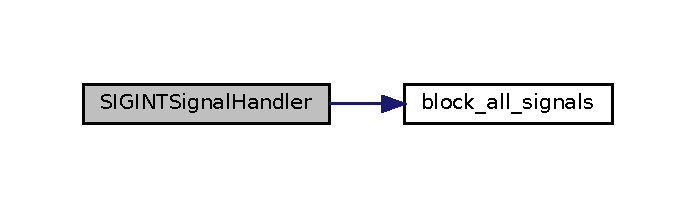
\includegraphics[width=350pt]{client_8h_a48d605ff689f470746c858648f0a98c2_cgraph}
\end{center}
\end{figure}
Questo è il grafo dei chiamanti di questa funzione\+:
\nopagebreak
\begin{figure}[H]
\begin{center}
\leavevmode
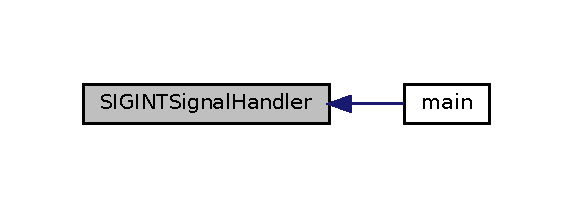
\includegraphics[width=275pt]{client_8h_a48d605ff689f470746c858648f0a98c2_icgraph}
\end{center}
\end{figure}
\mbox{\Hypertarget{client_8h_a50b22adcb76198fcd9402a97ff4711bf}\label{client_8h_a50b22adcb76198fcd9402a97ff4711bf}} 
\index{client.\+h@{client.\+h}!S\+I\+G\+U\+S\+R1\+Signal\+Handler@{S\+I\+G\+U\+S\+R1\+Signal\+Handler}}
\index{S\+I\+G\+U\+S\+R1\+Signal\+Handler@{S\+I\+G\+U\+S\+R1\+Signal\+Handler}!client.\+h@{client.\+h}}
\subsubsection{\texorpdfstring{S\+I\+G\+U\+S\+R1\+Signal\+Handler()}{SIGUSR1SignalHandler()}}
{\footnotesize\ttfamily void S\+I\+G\+U\+S\+R1\+Signal\+Handler (\begin{DoxyParamCaption}\item[{int}]{sig }\end{DoxyParamCaption})}



Handler del segnale S\+I\+G\+U\+S\+R1\+: chiude le risorse del client 0 e termina la sua esecuzione. 


\begin{DoxyParams}{Parametri}
{\em sig} & Valore intero corrispondente a S\+I\+G\+U\+S\+R1 \\
\hline
\end{DoxyParams}
Questo è il grafo delle chiamate per questa funzione\+:
\nopagebreak
\begin{figure}[H]
\begin{center}
\leavevmode
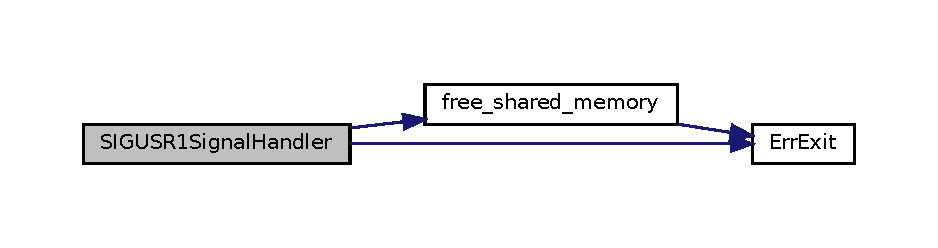
\includegraphics[width=350pt]{client_8h_a50b22adcb76198fcd9402a97ff4711bf_cgraph}
\end{center}
\end{figure}
Questo è il grafo dei chiamanti di questa funzione\+:
\nopagebreak
\begin{figure}[H]
\begin{center}
\leavevmode
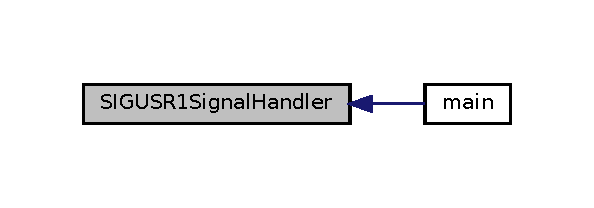
\includegraphics[width=285pt]{client_8h_a50b22adcb76198fcd9402a97ff4711bf_icgraph}
\end{center}
\end{figure}
\mbox{\Hypertarget{client_8h_ac129a55ffa08a55addb9ea1afbd709f8}\label{client_8h_ac129a55ffa08a55addb9ea1afbd709f8}} 
\index{client.\+h@{client.\+h}!str\+Equals@{str\+Equals}}
\index{str\+Equals@{str\+Equals}!client.\+h@{client.\+h}}
\subsubsection{\texorpdfstring{str\+Equals()}{strEquals()}}
{\footnotesize\ttfamily bool str\+Equals (\begin{DoxyParamCaption}\item[{char $\ast$}]{a,  }\item[{char $\ast$}]{b }\end{DoxyParamCaption})}

Restituisce vero se due stringhe sono uguali


\begin{DoxyParams}{Parametri}
{\em a} & Stringa da confrontare \\
\hline
{\em b} & Stringa da confrontare \\
\hline
\end{DoxyParams}
\begin{DoxyReturn}{Restituisce}
true a e b sono uguali 

false a e b sono diverse 
\end{DoxyReturn}
Questo è il grafo dei chiamanti di questa funzione\+:
\nopagebreak
\begin{figure}[H]
\begin{center}
\leavevmode
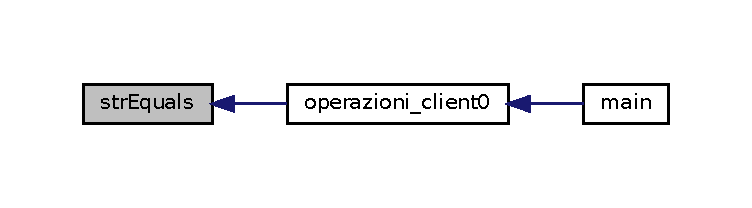
\includegraphics[width=350pt]{client_8h_ac129a55ffa08a55addb9ea1afbd709f8_icgraph}
\end{center}
\end{figure}

\hypertarget{defines_8c}{}\section{Riferimenti per il file /mnt/c/\+Users/stefa/\+Desktop/system\+\_\+call/src/defines.c}
\label{defines_8c}\index{/mnt/c/\+Users/stefa/\+Desktop/system\+\_\+call/src/defines.\+c@{/mnt/c/\+Users/stefa/\+Desktop/system\+\_\+call/src/defines.\+c}}


Contiene l\textquotesingle{}implementazione delle funzioni specifiche del progetto.  


{\ttfamily \#include \char`\"{}defines.\+h\char`\"{}}\newline
Grafo delle dipendenze di inclusione per defines.\+c\+:\nopagebreak
\begin{figure}[H]
\begin{center}
\leavevmode
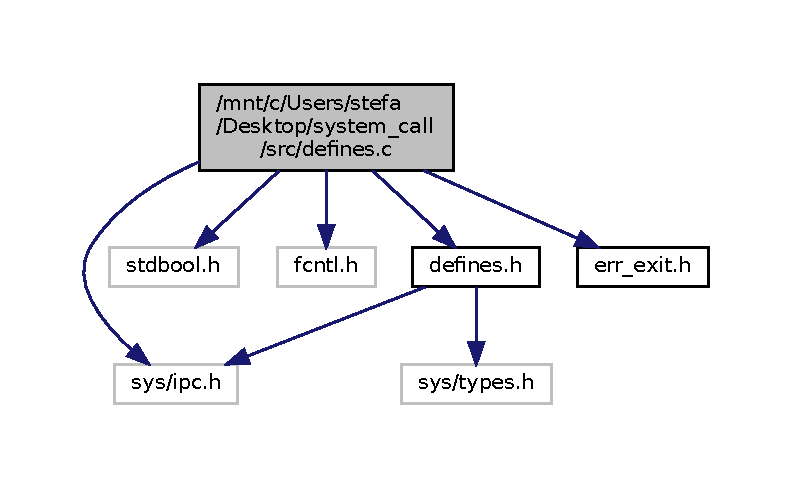
\includegraphics[width=202pt]{defines_8c__incl}
\end{center}
\end{figure}


\subsection{Descrizione dettagliata}
Contiene l\textquotesingle{}implementazione delle funzioni specifiche del progetto. 


\hypertarget{defines_8h}{}\section{Riferimenti per il file /mnt/c/\+Users/stefa/\+Desktop/system\+\_\+call/src/defines.h}
\label{defines_8h}\index{/mnt/c/\+Users/stefa/\+Desktop/system\+\_\+call/src/defines.\+h@{/mnt/c/\+Users/stefa/\+Desktop/system\+\_\+call/src/defines.\+h}}


Contiene la definizioni di variabili e funzioni specifiche del progetto.  


{\ttfamily \#include $<$sys/types.\+h$>$}\newline
{\ttfamily \#include $<$sys/ipc.\+h$>$}\newline
Grafo delle dipendenze di inclusione per defines.\+h\+:\nopagebreak
\begin{figure}[H]
\begin{center}
\leavevmode
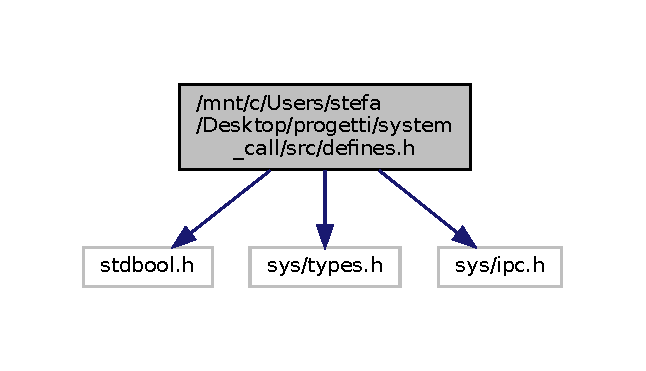
\includegraphics[width=230pt]{defines_8h__incl}
\end{center}
\end{figure}
Questo grafo mostra quali altri file includono direttamente o indirettamente questo file\+:
\nopagebreak
\begin{figure}[H]
\begin{center}
\leavevmode
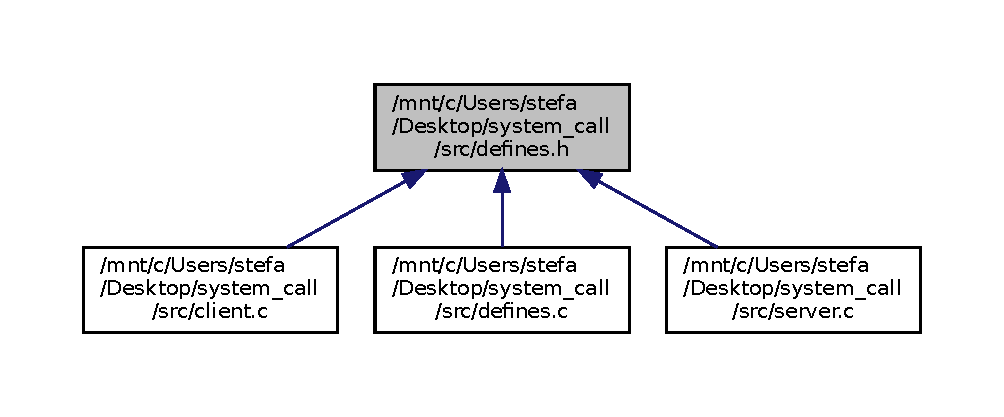
\includegraphics[width=350pt]{defines_8h__dep__incl}
\end{center}
\end{figure}
\subsection*{Strutture dati}
\begin{DoxyCompactItemize}
\item 
struct \hyperlink{structmsg__t}{msg\+\_\+t}
\end{DoxyCompactItemize}
\subsection*{Definizioni}
\begin{DoxyCompactItemize}
\item 
\mbox{\Hypertarget{defines_8h_a22ad48d95fdd6689ea92e17ca5bbfccb}\label{defines_8h_a22ad48d95fdd6689ea92e17ca5bbfccb}} 
\#define \hyperlink{defines_8h_a22ad48d95fdd6689ea92e17ca5bbfccb}{B\+U\+F\+F\+E\+R\+\_\+\+SZ}~255
\begin{DoxyCompactList}\small\item\em Buffer usato da getcwd() \end{DoxyCompactList}\item 
\mbox{\Hypertarget{defines_8h_a1e79a43e6110ccf4b3e3fcacc6e1a07e}\label{defines_8h_a1e79a43e6110ccf4b3e3fcacc6e1a07e}} 
\#define \hyperlink{defines_8h_a1e79a43e6110ccf4b3e3fcacc6e1a07e}{F\+I\+F\+O1\+\_\+\+P\+A\+TH}~\char`\"{}/tmp/fifo1\+\_\+file.\+txt\char`\"{}
\begin{DoxyCompactList}\small\item\em Percorso file F\+I\+FO 1. \end{DoxyCompactList}\item 
\mbox{\Hypertarget{defines_8h_a04902929b62d6decfed3e7ef544a5cdb}\label{defines_8h_a04902929b62d6decfed3e7ef544a5cdb}} 
\#define \hyperlink{defines_8h_a04902929b62d6decfed3e7ef544a5cdb}{F\+I\+F\+O2\+\_\+\+P\+A\+TH}~\char`\"{}/tmp/fifo2\+\_\+file.\+txt\char`\"{}
\begin{DoxyCompactList}\small\item\em Percorso file F\+I\+FO 2. \end{DoxyCompactList}\item 
\mbox{\Hypertarget{defines_8h_ac9f14b9a62477e207da30db724187294}\label{defines_8h_ac9f14b9a62477e207da30db724187294}} 
\#define \hyperlink{defines_8h_ac9f14b9a62477e207da30db724187294}{C\+O\+N\+T\+A\+I\+N\+S\+\_\+N}~1
\begin{DoxyCompactList}\small\item\em mtype messaggio che contiene numero di file \char`\"{}sendme\+\_\+\char`\"{} \end{DoxyCompactList}\item 
\mbox{\Hypertarget{defines_8h_a6667eab3262329122470b05145907db8}\label{defines_8h_a6667eab3262329122470b05145907db8}} 
\#define \hyperlink{defines_8h_a6667eab3262329122470b05145907db8}{C\+O\+N\+T\+A\+I\+N\+S\+\_\+\+F\+I\+F\+O1\+\_\+\+F\+I\+L\+E\+\_\+\+P\+A\+RT}~2
\begin{DoxyCompactList}\small\item\em mtype messaggio che contiene prima parte del contenuto del file \char`\"{}sendme\+\_\+\char`\"{} \end{DoxyCompactList}\item 
\mbox{\Hypertarget{defines_8h_a44b818300821c405cc58f8d0ad2da72b}\label{defines_8h_a44b818300821c405cc58f8d0ad2da72b}} 
\#define \hyperlink{defines_8h_a44b818300821c405cc58f8d0ad2da72b}{C\+O\+N\+T\+A\+I\+N\+S\+\_\+\+F\+I\+F\+O2\+\_\+\+F\+I\+L\+E\+\_\+\+P\+A\+RT}~3
\begin{DoxyCompactList}\small\item\em mtype messaggio che contiene seconda parte del contenuto del file \char`\"{}sendme\+\_\+\char`\"{} \end{DoxyCompactList}\item 
\mbox{\Hypertarget{defines_8h_a052160aa252d749598359d1908d1953d}\label{defines_8h_a052160aa252d749598359d1908d1953d}} 
\#define \hyperlink{defines_8h_a052160aa252d749598359d1908d1953d}{C\+O\+N\+T\+A\+I\+N\+S\+\_\+\+M\+S\+G\+Q\+U\+E\+U\+E\+\_\+\+F\+I\+L\+E\+\_\+\+P\+A\+RT}~4
\begin{DoxyCompactList}\small\item\em mtype messaggio che contiene terza parte del contenuto del file \char`\"{}sendme\+\_\+\char`\"{} \end{DoxyCompactList}\item 
\mbox{\Hypertarget{defines_8h_a170b91835f52208153fabe5086780cc1}\label{defines_8h_a170b91835f52208153fabe5086780cc1}} 
\#define \hyperlink{defines_8h_a170b91835f52208153fabe5086780cc1}{C\+O\+N\+T\+A\+I\+N\+S\+\_\+\+S\+H\+M\+\_\+\+F\+I\+L\+E\+\_\+\+P\+A\+RT}~5
\begin{DoxyCompactList}\small\item\em mtype messaggio che contiene quarta parte del contenuto del file \char`\"{}sendme\+\_\+\char`\"{} \end{DoxyCompactList}\item 
\mbox{\Hypertarget{defines_8h_a59b31ddb1f82961547749ce17239ada0}\label{defines_8h_a59b31ddb1f82961547749ce17239ada0}} 
\#define \hyperlink{defines_8h_a59b31ddb1f82961547749ce17239ada0}{C\+O\+N\+T\+A\+I\+N\+S\+\_\+\+D\+O\+NE}~6
\begin{DoxyCompactList}\small\item\em mtype messaggio che contiene il messaggio di fine proveniente dal server \end{DoxyCompactList}\item 
\mbox{\Hypertarget{defines_8h_ac4360beb7ee2bb020a085321d799418f}\label{defines_8h_ac4360beb7ee2bb020a085321d799418f}} 
\#define \hyperlink{defines_8h_ac4360beb7ee2bb020a085321d799418f}{I\+N\+I\+Z\+I\+A\+L\+I\+Z\+Z\+A\+Z\+I\+O\+N\+E\+\_\+\+M\+T\+Y\+PE}~-\/1
\begin{DoxyCompactList}\small\item\em mtype messaggio che contiene il valore usato per inizializzare la matrice contenente i file finali \end{DoxyCompactList}\item 
\mbox{\Hypertarget{defines_8h_a145b4c29c9494d8356c6108d9bf39aca}\label{defines_8h_a145b4c29c9494d8356c6108d9bf39aca}} 
\#define \hyperlink{defines_8h_a145b4c29c9494d8356c6108d9bf39aca}{M\+A\+X\+\_\+\+M\+S\+G\+\_\+\+P\+E\+R\+\_\+\+C\+H\+A\+N\+N\+EL}~50
\begin{DoxyCompactList}\small\item\em numero massimo di messaggi per canale di comunicazione \end{DoxyCompactList}\item 
\mbox{\Hypertarget{defines_8h_a0b8b71c287c99c2bd2e36f6bc95a005e}\label{defines_8h_a0b8b71c287c99c2bd2e36f6bc95a005e}} 
\#define \hyperlink{defines_8h_a0b8b71c287c99c2bd2e36f6bc95a005e}{M\+S\+G\+\_\+\+M\+A\+X\+\_\+\+SZ}~4096
\begin{DoxyCompactList}\small\item\em dimensione massima del messaggio/file da inviare \end{DoxyCompactList}\item 
\mbox{\Hypertarget{defines_8h_a2f72e71f34fb7e6074d029377ab31918}\label{defines_8h_a2f72e71f34fb7e6074d029377ab31918}} 
\#define \hyperlink{defines_8h_a2f72e71f34fb7e6074d029377ab31918}{M\+S\+G\+\_\+\+P\+A\+R\+T\+S\+\_\+\+N\+UM}~4
\begin{DoxyCompactList}\small\item\em numero parti in cui suddividere il messaggio \end{DoxyCompactList}\item 
\mbox{\Hypertarget{defines_8h_a46b84a677ff2bcf693b89247e39d75f7}\label{defines_8h_a46b84a677ff2bcf693b89247e39d75f7}} 
\#define \hyperlink{defines_8h_a46b84a677ff2bcf693b89247e39d75f7}{M\+S\+G\+\_\+\+B\+U\+F\+F\+E\+R\+\_\+\+SZ}~(\hyperlink{defines_8h_a0b8b71c287c99c2bd2e36f6bc95a005e}{M\+S\+G\+\_\+\+M\+A\+X\+\_\+\+SZ} / \hyperlink{defines_8h_a2f72e71f34fb7e6074d029377ab31918}{M\+S\+G\+\_\+\+P\+A\+R\+T\+S\+\_\+\+N\+UM})
\begin{DoxyCompactList}\small\item\em dimensione massima di una porzione di messaggio \end{DoxyCompactList}\end{DoxyCompactItemize}
\subsection*{Ridefinizioni di tipo (typedef)}
\begin{DoxyCompactItemize}
\item 
typedef struct \hyperlink{structmsg__t}{msg\+\_\+t} \hyperlink{defines_8h_a928de39fa56d656f7c6c92d030b36638}{msg\+\_\+t}
\end{DoxyCompactItemize}
\subsection*{Funzioni}
\begin{DoxyCompactItemize}
\item 
key\+\_\+t \hyperlink{defines_8h_a2d341373a96ffea0944553e5452cdbca}{get\+\_\+ipc\+\_\+key} ()
\item 
key\+\_\+t \hyperlink{defines_8h_afd25e0dffe44c8dd59ae86caabb94287}{get\+\_\+ipc\+\_\+key2} ()
\item 
key\+\_\+t \hyperlink{defines_8h_abe68b7232c057100c2e21586906436d7}{get\+\_\+project\+\_\+ipc\+\_\+key} (char proj\+\_\+id)
\item 
bool \hyperlink{defines_8h_ac281b05b7a90ba292f5748cbfe3c389d}{array\+Contains\+All\+True} (bool arr\mbox{[}$\,$\mbox{]}, int len)
\begin{DoxyCompactList}\small\item\em Restituisce vero se l\textquotesingle{}array contiene tutti true. \end{DoxyCompactList}\item 
int \hyperlink{defines_8h_aea9b93cad897755a46cb9e3373ba8cc2}{block\+FD} (int fd, int blocking)
\begin{DoxyCompactList}\small\item\em Rende bloccante oppure non bloccante un file descriptor. \end{DoxyCompactList}\end{DoxyCompactItemize}
\subsection*{Variabili}
\begin{DoxyCompactItemize}
\item 
\mbox{\Hypertarget{defines_8h_a709c4fcdc1217a8f8785cb59e85beee5}\label{defines_8h_a709c4fcdc1217a8f8785cb59e85beee5}} 
char \hyperlink{defines_8h_a709c4fcdc1217a8f8785cb59e85beee5}{E\+X\+E\+C\+U\+T\+A\+B\+L\+E\+\_\+\+D\+IR} \mbox{[}\hyperlink{defines_8h_a22ad48d95fdd6689ea92e17ca5bbfccb}{B\+U\+F\+F\+E\+R\+\_\+\+SZ}\mbox{]}
\begin{DoxyCompactList}\small\item\em Percorso cartella eseguibile. \end{DoxyCompactList}\end{DoxyCompactItemize}


\subsection{Descrizione dettagliata}
Contiene la definizioni di variabili e funzioni specifiche del progetto. 



\subsection{Documentazione delle ridefinizioni di tipo (typedef)}
\mbox{\Hypertarget{defines_8h_a928de39fa56d656f7c6c92d030b36638}\label{defines_8h_a928de39fa56d656f7c6c92d030b36638}} 
\index{defines.\+h@{defines.\+h}!msg\+\_\+t@{msg\+\_\+t}}
\index{msg\+\_\+t@{msg\+\_\+t}!defines.\+h@{defines.\+h}}
\subsubsection{\texorpdfstring{msg\+\_\+t}{msg\_t}}
{\footnotesize\ttfamily typedef struct \hyperlink{structmsg__t}{msg\+\_\+t}  \hyperlink{structmsg__t}{msg\+\_\+t}}

Rappresenta un messaggio contenente una porzione del contenuto di un file, il numero di file inviati dal client oppure il messaggio \char`\"{}ok\char`\"{} quando il server ha ricevuto il numero di file. 

\subsection{Documentazione delle funzioni}
\mbox{\Hypertarget{defines_8h_ac281b05b7a90ba292f5748cbfe3c389d}\label{defines_8h_ac281b05b7a90ba292f5748cbfe3c389d}} 
\index{defines.\+h@{defines.\+h}!array\+Contains\+All\+True@{array\+Contains\+All\+True}}
\index{array\+Contains\+All\+True@{array\+Contains\+All\+True}!defines.\+h@{defines.\+h}}
\subsubsection{\texorpdfstring{array\+Contains\+All\+True()}{arrayContainsAllTrue()}}
{\footnotesize\ttfamily bool array\+Contains\+All\+True (\begin{DoxyParamCaption}\item[{bool}]{arr\mbox{[}$\,$\mbox{]},  }\item[{int}]{len }\end{DoxyParamCaption})}



Restituisce vero se l\textquotesingle{}array contiene tutti true. 


\begin{DoxyParams}{Parametri}
{\em arr} & array di booleani \\
\hline
{\em len} & lunghezza array \\
\hline
\end{DoxyParams}
\begin{DoxyReturn}{Restituisce}
true arr contiene tutti true 

false arr contiene almeno un false 
\end{DoxyReturn}
Questo è il grafo dei chiamanti di questa funzione\+:\nopagebreak
\begin{figure}[H]
\begin{center}
\leavevmode
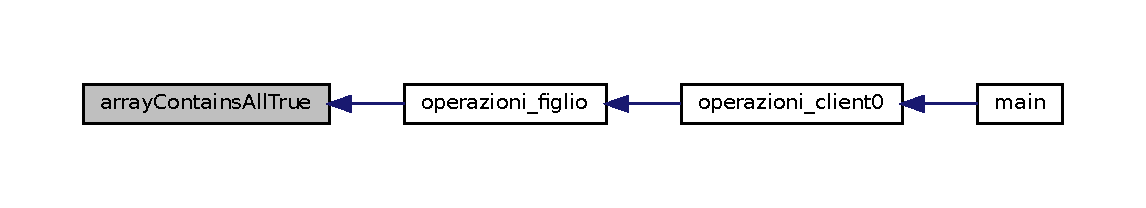
\includegraphics[width=350pt]{defines_8h_ac281b05b7a90ba292f5748cbfe3c389d_icgraph}
\end{center}
\end{figure}
\mbox{\Hypertarget{defines_8h_aea9b93cad897755a46cb9e3373ba8cc2}\label{defines_8h_aea9b93cad897755a46cb9e3373ba8cc2}} 
\index{defines.\+h@{defines.\+h}!block\+FD@{block\+FD}}
\index{block\+FD@{block\+FD}!defines.\+h@{defines.\+h}}
\subsubsection{\texorpdfstring{block\+F\+D()}{blockFD()}}
{\footnotesize\ttfamily int block\+FD (\begin{DoxyParamCaption}\item[{int}]{fd,  }\item[{int}]{blocking }\end{DoxyParamCaption})}



Rende bloccante oppure non bloccante un file descriptor. 


\begin{DoxyParams}{Parametri}
{\em fd} & file descriptor \\
\hline
{\em blocking} & 0\+: non bloccante, 1\+: bloccante \\
\hline
\end{DoxyParams}
\begin{DoxyReturn}{Restituisce}
int Vale 0 se fallisce 
\end{DoxyReturn}
Questo è il grafo dei chiamanti di questa funzione\+:\nopagebreak
\begin{figure}[H]
\begin{center}
\leavevmode
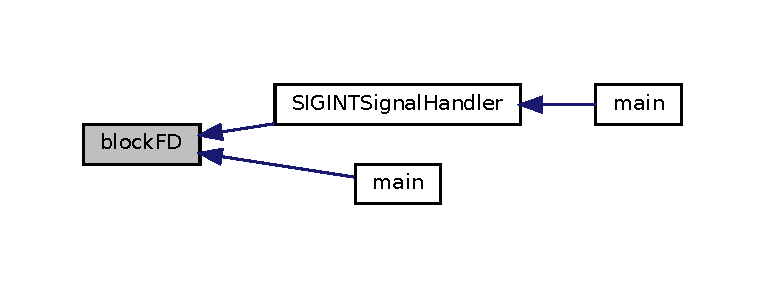
\includegraphics[width=350pt]{defines_8h_aea9b93cad897755a46cb9e3373ba8cc2_icgraph}
\end{center}
\end{figure}
\mbox{\Hypertarget{defines_8h_a2d341373a96ffea0944553e5452cdbca}\label{defines_8h_a2d341373a96ffea0944553e5452cdbca}} 
\index{defines.\+h@{defines.\+h}!get\+\_\+ipc\+\_\+key@{get\+\_\+ipc\+\_\+key}}
\index{get\+\_\+ipc\+\_\+key@{get\+\_\+ipc\+\_\+key}!defines.\+h@{defines.\+h}}
\subsubsection{\texorpdfstring{get\+\_\+ipc\+\_\+key()}{get\_ipc\_key()}}
{\footnotesize\ttfamily key\+\_\+t get\+\_\+ipc\+\_\+key (\begin{DoxyParamCaption}{ }\end{DoxyParamCaption})}

Restituisce la prima chiave I\+PC ottenuta con \hyperlink{defines_8h_abe68b7232c057100c2e21586906436d7}{get\+\_\+project\+\_\+ipc\+\_\+key()}.

\begin{DoxyReturn}{Restituisce}
key\+\_\+t Chiave I\+PC 
\end{DoxyReturn}
Questo è il grafo delle chiamate per questa funzione\+:\nopagebreak
\begin{figure}[H]
\begin{center}
\leavevmode
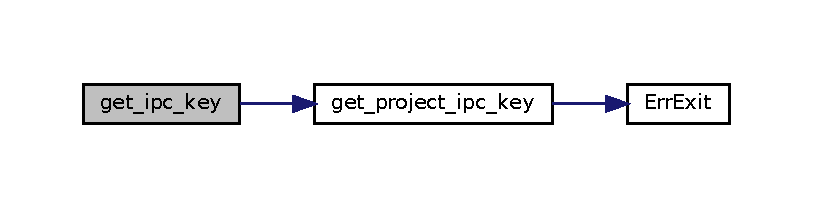
\includegraphics[width=350pt]{defines_8h_a2d341373a96ffea0944553e5452cdbca_cgraph}
\end{center}
\end{figure}
Questo è il grafo dei chiamanti di questa funzione\+:\nopagebreak
\begin{figure}[H]
\begin{center}
\leavevmode
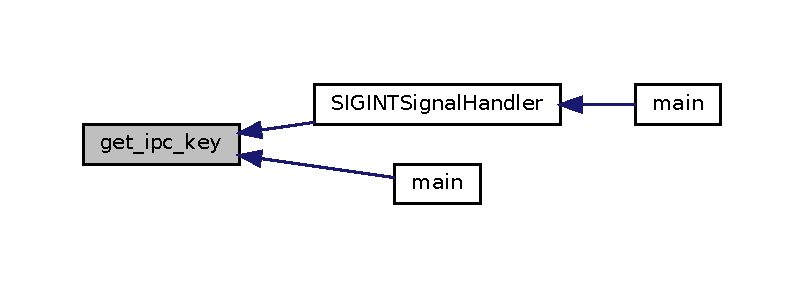
\includegraphics[width=350pt]{defines_8h_a2d341373a96ffea0944553e5452cdbca_icgraph}
\end{center}
\end{figure}
\mbox{\Hypertarget{defines_8h_afd25e0dffe44c8dd59ae86caabb94287}\label{defines_8h_afd25e0dffe44c8dd59ae86caabb94287}} 
\index{defines.\+h@{defines.\+h}!get\+\_\+ipc\+\_\+key2@{get\+\_\+ipc\+\_\+key2}}
\index{get\+\_\+ipc\+\_\+key2@{get\+\_\+ipc\+\_\+key2}!defines.\+h@{defines.\+h}}
\subsubsection{\texorpdfstring{get\+\_\+ipc\+\_\+key2()}{get\_ipc\_key2()}}
{\footnotesize\ttfamily key\+\_\+t get\+\_\+ipc\+\_\+key2 (\begin{DoxyParamCaption}{ }\end{DoxyParamCaption})}

Restituisce la seconda chiave I\+PC ottenuta con \hyperlink{defines_8h_abe68b7232c057100c2e21586906436d7}{get\+\_\+project\+\_\+ipc\+\_\+key()}.

\begin{DoxyReturn}{Restituisce}
key\+\_\+t Chiave I\+PC 
\end{DoxyReturn}
Questo è il grafo delle chiamate per questa funzione\+:\nopagebreak
\begin{figure}[H]
\begin{center}
\leavevmode
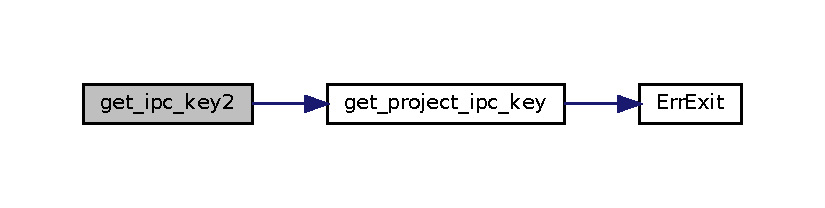
\includegraphics[width=350pt]{defines_8h_afd25e0dffe44c8dd59ae86caabb94287_cgraph}
\end{center}
\end{figure}
Questo è il grafo dei chiamanti di questa funzione\+:\nopagebreak
\begin{figure}[H]
\begin{center}
\leavevmode
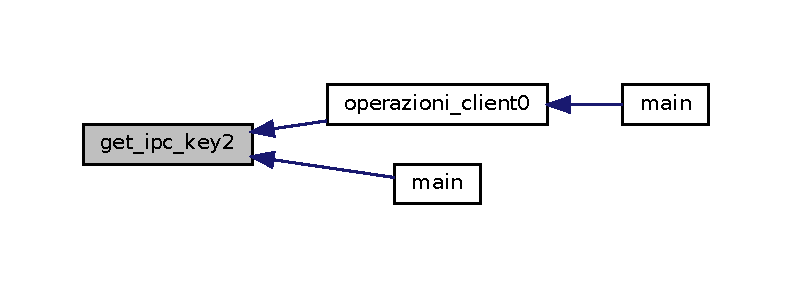
\includegraphics[width=350pt]{defines_8h_afd25e0dffe44c8dd59ae86caabb94287_icgraph}
\end{center}
\end{figure}
\mbox{\Hypertarget{defines_8h_abe68b7232c057100c2e21586906436d7}\label{defines_8h_abe68b7232c057100c2e21586906436d7}} 
\index{defines.\+h@{defines.\+h}!get\+\_\+project\+\_\+ipc\+\_\+key@{get\+\_\+project\+\_\+ipc\+\_\+key}}
\index{get\+\_\+project\+\_\+ipc\+\_\+key@{get\+\_\+project\+\_\+ipc\+\_\+key}!defines.\+h@{defines.\+h}}
\subsubsection{\texorpdfstring{get\+\_\+project\+\_\+ipc\+\_\+key()}{get\_project\_ipc\_key()}}
{\footnotesize\ttfamily key\+\_\+t get\+\_\+project\+\_\+ipc\+\_\+key (\begin{DoxyParamCaption}\item[{char}]{proj\+\_\+id }\end{DoxyParamCaption})}

Restituisce una chiave I\+PC generica per il progetto ottenuta con ftok sulla cartella con gli eseguibili.

\begin{DoxyReturn}{Restituisce}
key\+\_\+t Chiave I\+PC 
\end{DoxyReturn}
Questo è il grafo delle chiamate per questa funzione\+:\nopagebreak
\begin{figure}[H]
\begin{center}
\leavevmode
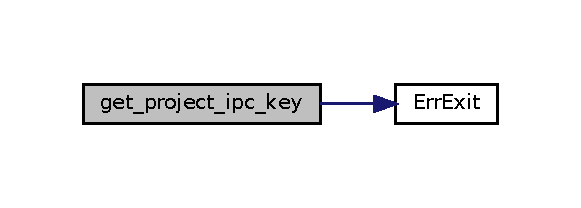
\includegraphics[width=279pt]{defines_8h_abe68b7232c057100c2e21586906436d7_cgraph}
\end{center}
\end{figure}
Questo è il grafo dei chiamanti di questa funzione\+:\nopagebreak
\begin{figure}[H]
\begin{center}
\leavevmode
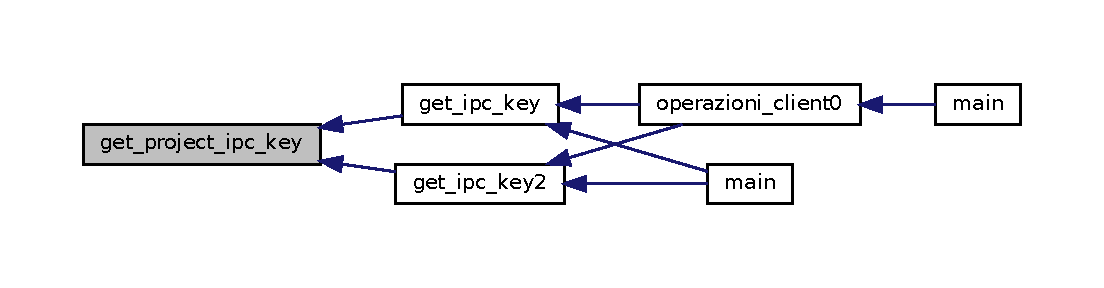
\includegraphics[width=350pt]{defines_8h_abe68b7232c057100c2e21586906436d7_icgraph}
\end{center}
\end{figure}

\hypertarget{err__exit_8c}{}\section{Riferimenti per il file /mnt/c/\+Users/stefa/\+Desktop/new/system\+\_\+call/src/err\+\_\+exit.c}
\label{err__exit_8c}\index{/mnt/c/\+Users/stefa/\+Desktop/new/system\+\_\+call/src/err\+\_\+exit.\+c@{/mnt/c/\+Users/stefa/\+Desktop/new/system\+\_\+call/src/err\+\_\+exit.\+c}}


Contiene l\textquotesingle{}implementazione della funzione di stampa degli errori.  


{\ttfamily \#include \char`\"{}err\+\_\+exit.\+h\char`\"{}}\newline
{\ttfamily \#include $<$stdlib.\+h$>$}\newline
{\ttfamily \#include $<$stdarg.\+h$>$}\newline
{\ttfamily \#include $<$stdio.\+h$>$}\newline
{\ttfamily \#include $<$errno.\+h$>$}\newline
Grafo delle dipendenze di inclusione per err\+\_\+exit.\+c\+:
\nopagebreak
\begin{figure}[H]
\begin{center}
\leavevmode
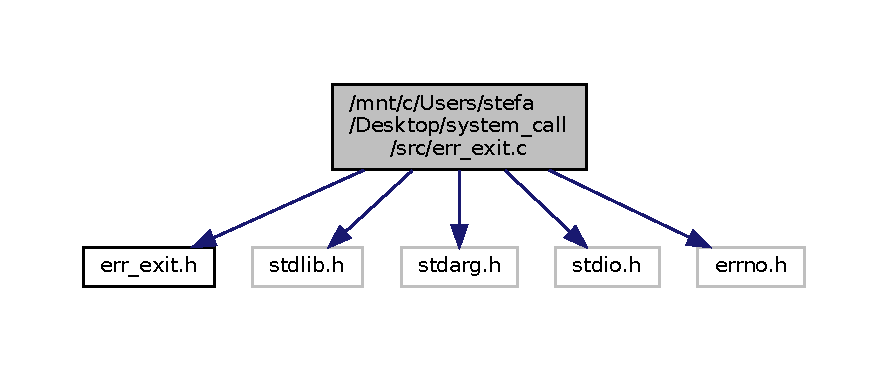
\includegraphics[width=350pt]{err__exit_8c__incl}
\end{center}
\end{figure}
\subsection*{Funzioni}
\begin{DoxyCompactItemize}
\item 
\mbox{\Hypertarget{err__exit_8c_aa223b0ecfe538d130ece562646a37d27}\label{err__exit_8c_aa223b0ecfe538d130ece562646a37d27}} 
void \hyperlink{err__exit_8c_aa223b0ecfe538d130ece562646a37d27}{Err\+Exit} (const char $\ast$msg)
\begin{DoxyCompactList}\small\item\em Prints the error message of the last failed system call and terminates the calling process. \end{DoxyCompactList}\end{DoxyCompactItemize}


\subsection{Descrizione dettagliata}
Contiene l\textquotesingle{}implementazione della funzione di stampa degli errori. 


\hypertarget{err__exit_8h}{}\section{Riferimenti per il file /mnt/c/\+Users/stefa/\+Desktop/system\+\_\+call/src/err\+\_\+exit.h}
\label{err__exit_8h}\index{/mnt/c/\+Users/stefa/\+Desktop/system\+\_\+call/src/err\+\_\+exit.\+h@{/mnt/c/\+Users/stefa/\+Desktop/system\+\_\+call/src/err\+\_\+exit.\+h}}


Contiene la definizione della funzione di stampa degli errori.  


Questo grafo mostra quali altri file includono direttamente o indirettamente questo file\+:\nopagebreak
\begin{figure}[H]
\begin{center}
\leavevmode
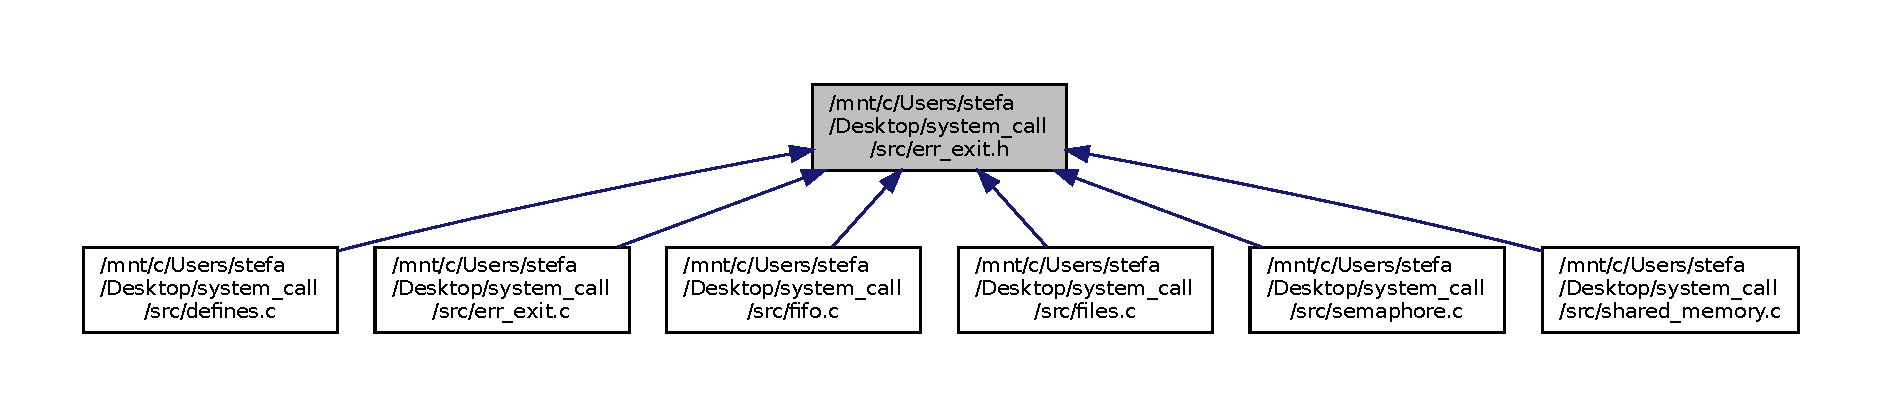
\includegraphics[width=350pt]{err__exit_8h__dep__incl}
\end{center}
\end{figure}
\subsection*{Funzioni}
\begin{DoxyCompactItemize}
\item 
\mbox{\Hypertarget{err__exit_8h_aa223b0ecfe538d130ece562646a37d27}\label{err__exit_8h_aa223b0ecfe538d130ece562646a37d27}} 
void \hyperlink{err__exit_8h_aa223b0ecfe538d130ece562646a37d27}{Err\+Exit} (const char $\ast$msg)
\begin{DoxyCompactList}\small\item\em Prints the error message of the last failed system call and terminates the calling process. \end{DoxyCompactList}\end{DoxyCompactItemize}


\subsection{Descrizione dettagliata}
Contiene la definizione della funzione di stampa degli errori. 


\hypertarget{fifo_8c}{}\section{Riferimenti per il file /mnt/c/\+Users/stefa/\+Desktop/progetti/system\+\_\+call/src/fifo.c}
\label{fifo_8c}\index{/mnt/c/\+Users/stefa/\+Desktop/progetti/system\+\_\+call/src/fifo.\+c@{/mnt/c/\+Users/stefa/\+Desktop/progetti/system\+\_\+call/src/fifo.\+c}}


Contiene l\textquotesingle{}implementazione delle funzioni specifiche per la gestione delle F\+I\+FO.  


{\ttfamily \#include $<$stdlib.\+h$>$}\newline
{\ttfamily \#include $<$stdio.\+h$>$}\newline
{\ttfamily \#include $<$sys/ipc.\+h$>$}\newline
{\ttfamily \#include $<$sys/stat.\+h$>$}\newline
{\ttfamily \#include $<$fcntl.\+h$>$}\newline
{\ttfamily \#include $<$errno.\+h$>$}\newline
{\ttfamily \#include $<$unistd.\+h$>$}\newline
{\ttfamily \#include \char`\"{}err\+\_\+exit.\+h\char`\"{}}\newline
{\ttfamily \#include \char`\"{}fifo.\+h\char`\"{}}\newline
{\ttfamily \#include \char`\"{}debug.\+h\char`\"{}}\newline
{\ttfamily \#include \char`\"{}defines.\+h\char`\"{}}\newline
Grafo delle dipendenze di inclusione per fifo.\+c\+:
\nopagebreak
\begin{figure}[H]
\begin{center}
\leavevmode
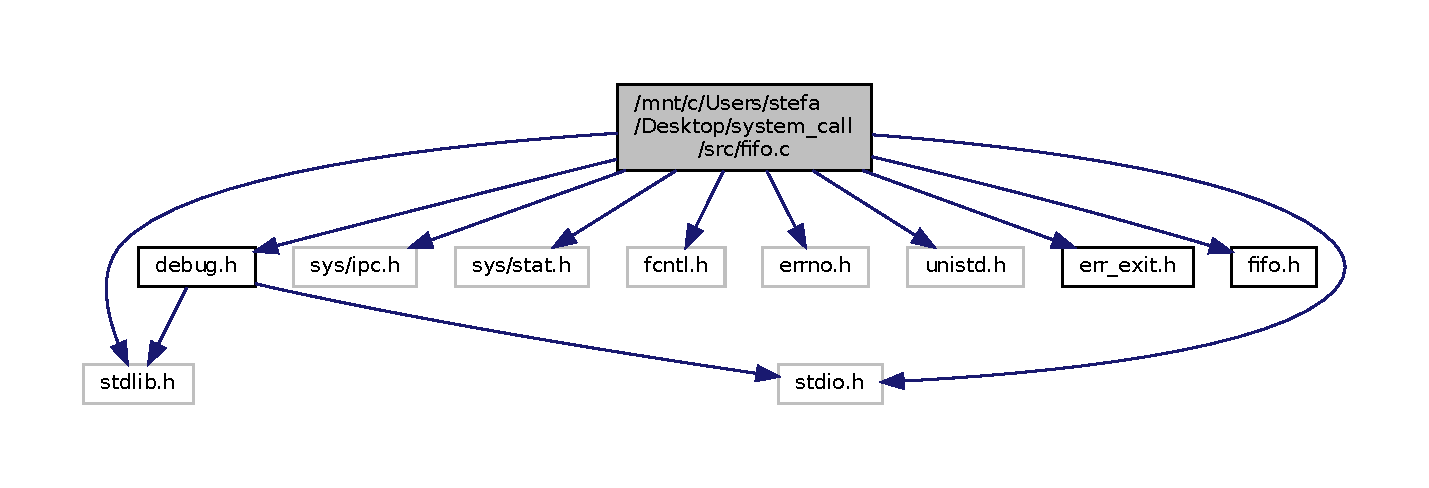
\includegraphics[width=350pt]{fifo_8c__incl}
\end{center}
\end{figure}
\subsection*{Funzioni}
\begin{DoxyCompactItemize}
\item 
void \hyperlink{fifo_8c_ab83de0eb3bc3947e3c031685d5c2474b}{make\+\_\+fifo} (char $\ast$path)
\begin{DoxyCompactList}\small\item\em Crea o ottiene una I\+PC F\+I\+FO usando mkfifo. \end{DoxyCompactList}\item 
int \hyperlink{fifo_8c_a54a1ae8162825128cf02f95692402c18}{create\+\_\+fifo} (char $\ast$path, char mode)
\begin{DoxyCompactList}\small\item\em Facilita la creazione di una F\+I\+FO (o ne ottiene una esistente) in modalita\textquotesingle{} lettura o scrittura. \end{DoxyCompactList}\end{DoxyCompactItemize}


\subsection{Descrizione dettagliata}
Contiene l\textquotesingle{}implementazione delle funzioni specifiche per la gestione delle F\+I\+FO. 



\subsection{Documentazione delle funzioni}
\mbox{\Hypertarget{fifo_8c_a54a1ae8162825128cf02f95692402c18}\label{fifo_8c_a54a1ae8162825128cf02f95692402c18}} 
\index{fifo.\+c@{fifo.\+c}!create\+\_\+fifo@{create\+\_\+fifo}}
\index{create\+\_\+fifo@{create\+\_\+fifo}!fifo.\+c@{fifo.\+c}}
\subsubsection{\texorpdfstring{create\+\_\+fifo()}{create\_fifo()}}
{\footnotesize\ttfamily int create\+\_\+fifo (\begin{DoxyParamCaption}\item[{char $\ast$}]{path,  }\item[{char}]{mode }\end{DoxyParamCaption})}



Facilita la creazione di una F\+I\+FO (o ne ottiene una esistente) in modalita\textquotesingle{} lettura o scrittura. 


\begin{DoxyParams}{Parametri}
{\em path} & Percorso file usato dalla F\+I\+FO. \\
\hline
{\em mode} & \textquotesingle{}r\textquotesingle{} (read) oppure \textquotesingle{}w\textquotesingle{} (write) \\
\hline
\end{DoxyParams}
\begin{DoxyReturn}{Restituisce}
int Descrittore della F\+I\+FO 
\end{DoxyReturn}
Questo è il grafo delle chiamate per questa funzione\+:
\nopagebreak
\begin{figure}[H]
\begin{center}
\leavevmode
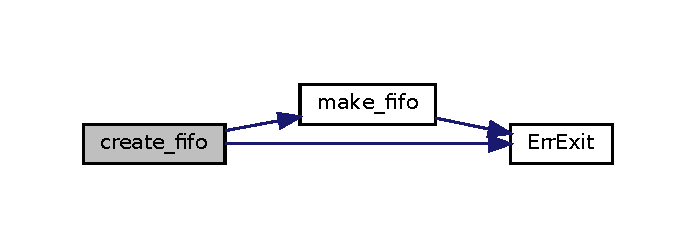
\includegraphics[width=334pt]{fifo_8c_a54a1ae8162825128cf02f95692402c18_cgraph}
\end{center}
\end{figure}
Questo è il grafo dei chiamanti di questa funzione\+:
\nopagebreak
\begin{figure}[H]
\begin{center}
\leavevmode
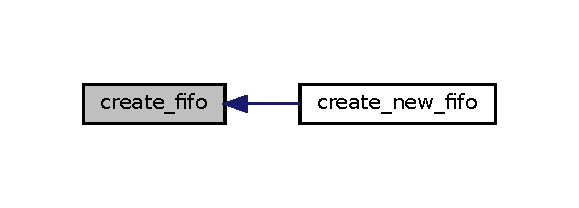
\includegraphics[width=350pt]{fifo_8c_a54a1ae8162825128cf02f95692402c18_icgraph}
\end{center}
\end{figure}
\mbox{\Hypertarget{fifo_8c_ab83de0eb3bc3947e3c031685d5c2474b}\label{fifo_8c_ab83de0eb3bc3947e3c031685d5c2474b}} 
\index{fifo.\+c@{fifo.\+c}!make\+\_\+fifo@{make\+\_\+fifo}}
\index{make\+\_\+fifo@{make\+\_\+fifo}!fifo.\+c@{fifo.\+c}}
\subsubsection{\texorpdfstring{make\+\_\+fifo()}{make\_fifo()}}
{\footnotesize\ttfamily void make\+\_\+fifo (\begin{DoxyParamCaption}\item[{char $\ast$}]{path }\end{DoxyParamCaption})}



Crea o ottiene una I\+PC F\+I\+FO usando mkfifo. 


\begin{DoxyParams}{Parametri}
{\em path} & Percorso file usato dalla F\+I\+FO. \\
\hline
\end{DoxyParams}
Questo è il grafo delle chiamate per questa funzione\+:
\nopagebreak
\begin{figure}[H]
\begin{center}
\leavevmode
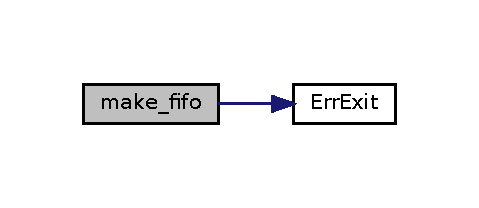
\includegraphics[width=230pt]{fifo_8c_ab83de0eb3bc3947e3c031685d5c2474b_cgraph}
\end{center}
\end{figure}
Questo è il grafo dei chiamanti di questa funzione\+:
\nopagebreak
\begin{figure}[H]
\begin{center}
\leavevmode
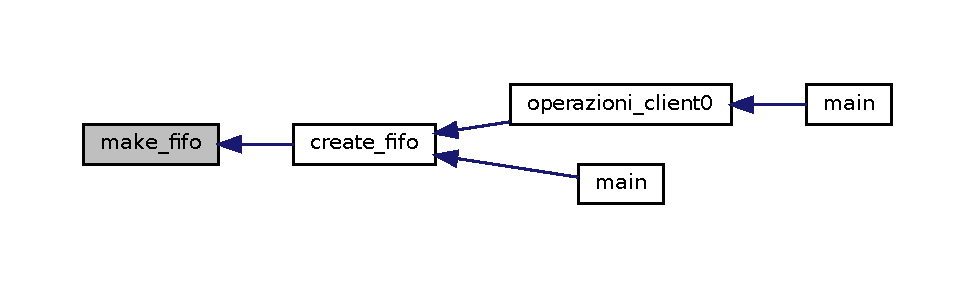
\includegraphics[width=350pt]{fifo_8c_ab83de0eb3bc3947e3c031685d5c2474b_icgraph}
\end{center}
\end{figure}

\hypertarget{fifo_8h}{}\section{Riferimenti per il file /mnt/c/\+Users/stefa/\+Desktop/system\+\_\+call/src/fifo.h}
\label{fifo_8h}\index{/mnt/c/\+Users/stefa/\+Desktop/system\+\_\+call/src/fifo.\+h@{/mnt/c/\+Users/stefa/\+Desktop/system\+\_\+call/src/fifo.\+h}}


Contiene la definizioni di variabili e funzioni specifiche per la gestione delle F\+I\+FO.  


Questo grafo mostra quali altri file includono direttamente o indirettamente questo file\+:\nopagebreak
\begin{figure}[H]
\begin{center}
\leavevmode
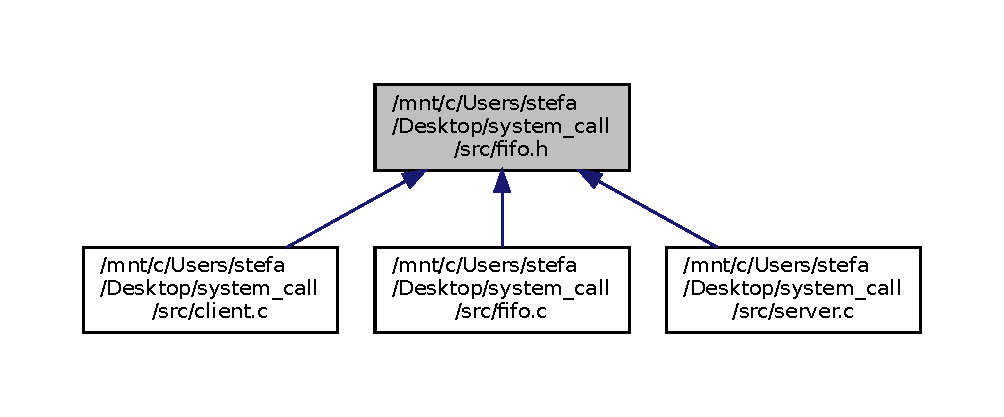
\includegraphics[width=342pt]{fifo_8h__dep__incl}
\end{center}
\end{figure}


\subsection{Descrizione dettagliata}
Contiene la definizioni di variabili e funzioni specifiche per la gestione delle F\+I\+FO. 


\hypertarget{files_8c}{}\section{Riferimenti per il file /mnt/c/\+Users/stefa/\+Desktop/new/system\+\_\+call/src/files.c}
\label{files_8c}\index{/mnt/c/\+Users/stefa/\+Desktop/new/system\+\_\+call/src/files.\+c@{/mnt/c/\+Users/stefa/\+Desktop/new/system\+\_\+call/src/files.\+c}}


Contiene le funzioni specifiche per la gestione dei F\+I\+LE.  


{\ttfamily \#include $<$stdlib.\+h$>$}\newline
{\ttfamily \#include $<$sys/stat.\+h$>$}\newline
{\ttfamily \#include $<$dirent.\+h$>$}\newline
{\ttfamily \#include $<$errno.\+h$>$}\newline
{\ttfamily \#include $<$stdio.\+h$>$}\newline
{\ttfamily \#include $<$string.\+h$>$}\newline
{\ttfamily \#include \char`\"{}strings.\+h\char`\"{}}\newline
{\ttfamily \#include \char`\"{}files.\+h\char`\"{}}\newline
{\ttfamily \#include \char`\"{}err\+\_\+exit.\+h\char`\"{}}\newline
{\ttfamily \#include \char`\"{}debug.\+h\char`\"{}}\newline
Grafo delle dipendenze di inclusione per files.\+c\+:
\nopagebreak
\begin{figure}[H]
\begin{center}
\leavevmode
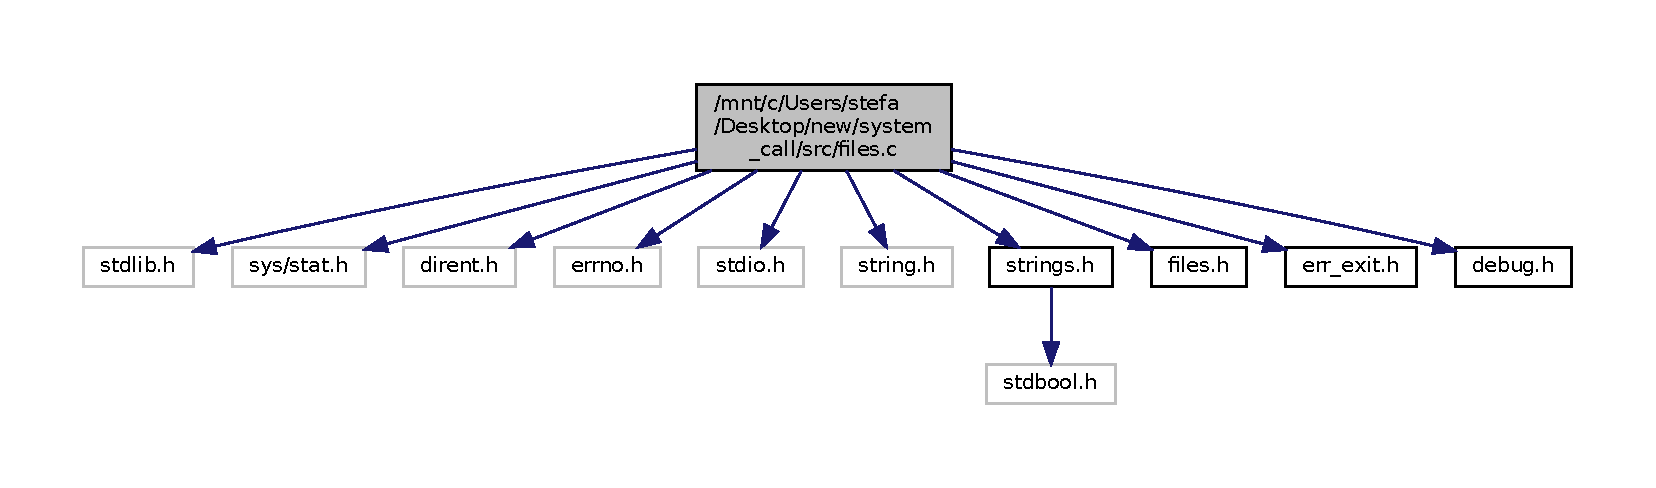
\includegraphics[width=350pt]{files_8c__incl}
\end{center}
\end{figure}
\subsection*{Funzioni}
\begin{DoxyCompactItemize}
\item 
void \hyperlink{files_8c_a1cdd9b5b37408e31d80f31e474a71483}{print\+\_\+list} (\hyperlink{structfiles__list}{files\+\_\+list} $\ast$head)
\begin{DoxyCompactList}\small\item\em Visualizza il contenuto della lista concatenata di file\+Path. \end{DoxyCompactList}\item 
\hyperlink{structfiles__list}{files\+\_\+list} $\ast$ \hyperlink{files_8c_a6a46f37bcdbf048db0fba5bb3e0e6342}{append} (\hyperlink{structfiles__list}{files\+\_\+list} $\ast$head, char $\ast$path)
\begin{DoxyCompactList}\small\item\em Aggiunge in fondo alla coda un nuovo file\+Path. \end{DoxyCompactList}\item 
void \hyperlink{files_8c_a786a7b6f9c01e8489d7196a79f5f3862}{free\+\_\+list} (\hyperlink{structfiles__list}{files\+\_\+list} $\ast$head)
\begin{DoxyCompactList}\small\item\em Libera la memoria dello H\+E\+AP occupata dalla lista di file\+Path. \end{DoxyCompactList}\item 
int \hyperlink{files_8c_a3ba19f05c37434e7f20facff3445651a}{count\+\_\+files} (\hyperlink{structfiles__list}{files\+\_\+list} $\ast$head)
\begin{DoxyCompactList}\small\item\em Conta il numero di file nella lista concatenata di file\+Path. \end{DoxyCompactList}\item 
long \hyperlink{files_8c_a096f8e9259afb2839ebe6822364f9928}{get\+File\+Size} (char $\ast$file\+Path)
\begin{DoxyCompactList}\small\item\em Restituisce dimensione del file in byte. \end{DoxyCompactList}\item 
int \hyperlink{files_8c_a5ac4517096592013308a3252f3226f60}{check\+File\+Size} (char $\ast$file\+Path)
\begin{DoxyCompactList}\small\item\em Restituisce 1 se il percorso ha la dimensione $<$= 4 KB, 0 altrimenti. \end{DoxyCompactList}\item 
int \hyperlink{files_8c_a675d61c6bfe0d9ddd1be59233dfd7d5c}{check\+File\+Name} (char $\ast$file\+Name)
\begin{DoxyCompactList}\small\item\em Restituisce 1 se il percorso inizia con \char`\"{}sendme\+\_\+\char`\"{}, 0 altrimenti. \end{DoxyCompactList}\item 
\hyperlink{structfiles__list}{files\+\_\+list} $\ast$ \hyperlink{files_8c_a627e4b202ea71f3bd241ccf562449bd6}{find\+\_\+sendme\+\_\+files} (char $\ast$search\+Path, \hyperlink{structfiles__list}{files\+\_\+list} $\ast$head)
\end{DoxyCompactItemize}


\subsection{Descrizione dettagliata}
Contiene le funzioni specifiche per la gestione dei F\+I\+LE. 



\subsection{Documentazione delle funzioni}
\mbox{\Hypertarget{files_8c_a6a46f37bcdbf048db0fba5bb3e0e6342}\label{files_8c_a6a46f37bcdbf048db0fba5bb3e0e6342}} 
\index{files.\+c@{files.\+c}!append@{append}}
\index{append@{append}!files.\+c@{files.\+c}}
\subsubsection{\texorpdfstring{append()}{append()}}
{\footnotesize\ttfamily \hyperlink{structfiles__list}{files\+\_\+list}$\ast$ append (\begin{DoxyParamCaption}\item[{\hyperlink{structfiles__list}{files\+\_\+list} $\ast$}]{head,  }\item[{char $\ast$}]{path }\end{DoxyParamCaption})}



Aggiunge in fondo alla coda un nuovo file\+Path. 


\begin{DoxyParams}{Parametri}
{\em head} & Nodo di testa della coda \\
\hline
{\em path} & file\+Path da aggiungere in fondo \\
\hline
\end{DoxyParams}
\begin{DoxyReturn}{Restituisce}
files\+\_\+list$\ast$ Nodo di testa della coda (se head == N\+U\+LL verra\textquotesingle{} creato il primo nodo) 
\end{DoxyReturn}
Questo è il grafo dei chiamanti di questa funzione\+:\nopagebreak
\begin{figure}[H]
\begin{center}
\leavevmode
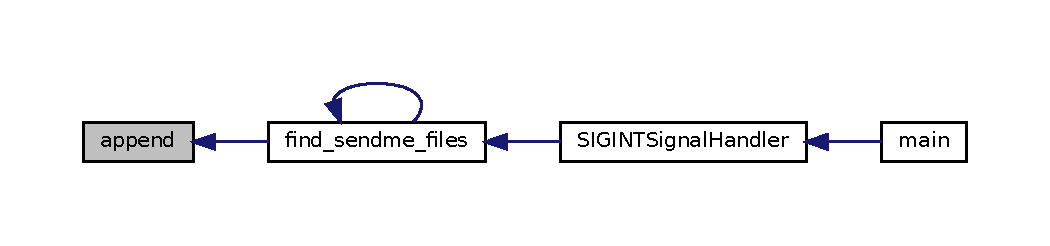
\includegraphics[width=273pt]{files_8c_a6a46f37bcdbf048db0fba5bb3e0e6342_icgraph}
\end{center}
\end{figure}
\mbox{\Hypertarget{files_8c_a675d61c6bfe0d9ddd1be59233dfd7d5c}\label{files_8c_a675d61c6bfe0d9ddd1be59233dfd7d5c}} 
\index{files.\+c@{files.\+c}!check\+File\+Name@{check\+File\+Name}}
\index{check\+File\+Name@{check\+File\+Name}!files.\+c@{files.\+c}}
\subsubsection{\texorpdfstring{check\+File\+Name()}{checkFileName()}}
{\footnotesize\ttfamily int check\+File\+Name (\begin{DoxyParamCaption}\item[{char $\ast$}]{file\+Name }\end{DoxyParamCaption})}



Restituisce 1 se il percorso inizia con \char`\"{}sendme\+\_\+\char`\"{}, 0 altrimenti. 


\begin{DoxyParams}{Parametri}
{\em file\+Name} & Percorso del file \\
\hline
\end{DoxyParams}
\begin{DoxyReturn}{Restituisce}
int Vale 1 se il percorso inizia con \char`\"{}sendme\+\_\+\char`\"{}, 0 altrimenti 
\end{DoxyReturn}
Questo è il grafo delle chiamate per questa funzione\+:\nopagebreak
\begin{figure}[H]
\begin{center}
\leavevmode
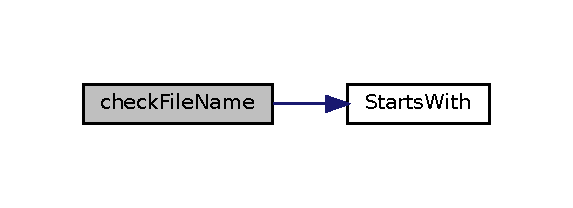
\includegraphics[width=275pt]{files_8c_a675d61c6bfe0d9ddd1be59233dfd7d5c_cgraph}
\end{center}
\end{figure}
Questo è il grafo dei chiamanti di questa funzione\+:\nopagebreak
\begin{figure}[H]
\begin{center}
\leavevmode
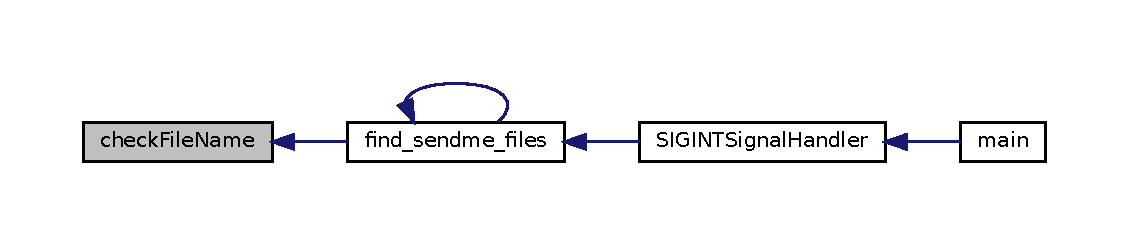
\includegraphics[width=311pt]{files_8c_a675d61c6bfe0d9ddd1be59233dfd7d5c_icgraph}
\end{center}
\end{figure}
\mbox{\Hypertarget{files_8c_a5ac4517096592013308a3252f3226f60}\label{files_8c_a5ac4517096592013308a3252f3226f60}} 
\index{files.\+c@{files.\+c}!check\+File\+Size@{check\+File\+Size}}
\index{check\+File\+Size@{check\+File\+Size}!files.\+c@{files.\+c}}
\subsubsection{\texorpdfstring{check\+File\+Size()}{checkFileSize()}}
{\footnotesize\ttfamily int check\+File\+Size (\begin{DoxyParamCaption}\item[{char $\ast$}]{file\+Path }\end{DoxyParamCaption})}



Restituisce 1 se il percorso ha la dimensione $<$= 4 KB, 0 altrimenti. 


\begin{DoxyParams}{Parametri}
{\em file\+Path} & Percorso del file \\
\hline
\end{DoxyParams}
\begin{DoxyReturn}{Restituisce}
int Vale 1 se il percorso ha la dimensione $<$= 4 KB, 0 altrimenti 
\end{DoxyReturn}
Questo è il grafo delle chiamate per questa funzione\+:\nopagebreak
\begin{figure}[H]
\begin{center}
\leavevmode
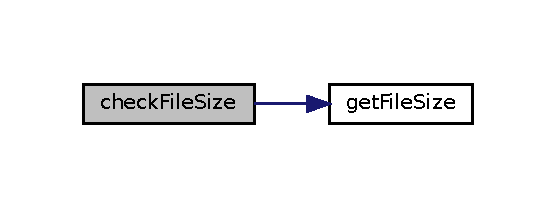
\includegraphics[width=267pt]{files_8c_a5ac4517096592013308a3252f3226f60_cgraph}
\end{center}
\end{figure}
Questo è il grafo dei chiamanti di questa funzione\+:\nopagebreak
\begin{figure}[H]
\begin{center}
\leavevmode
\includegraphics[width=302pt]{files_8c_a5ac4517096592013308a3252f3226f60_icgraph}
\end{center}
\end{figure}
\mbox{\Hypertarget{files_8c_a3ba19f05c37434e7f20facff3445651a}\label{files_8c_a3ba19f05c37434e7f20facff3445651a}} 
\index{files.\+c@{files.\+c}!count\+\_\+files@{count\+\_\+files}}
\index{count\+\_\+files@{count\+\_\+files}!files.\+c@{files.\+c}}
\subsubsection{\texorpdfstring{count\+\_\+files()}{count\_files()}}
{\footnotesize\ttfamily int count\+\_\+files (\begin{DoxyParamCaption}\item[{\hyperlink{structfiles__list}{files\+\_\+list} $\ast$}]{head }\end{DoxyParamCaption})}



Conta il numero di file nella lista concatenata di file\+Path. 


\begin{DoxyParams}{Parametri}
{\em head} & Nodo di testa della coda \\
\hline
\end{DoxyParams}
\begin{DoxyReturn}{Restituisce}
int Numero di file 
\end{DoxyReturn}
\mbox{\Hypertarget{files_8c_a627e4b202ea71f3bd241ccf562449bd6}\label{files_8c_a627e4b202ea71f3bd241ccf562449bd6}} 
\index{files.\+c@{files.\+c}!find\+\_\+sendme\+\_\+files@{find\+\_\+sendme\+\_\+files}}
\index{find\+\_\+sendme\+\_\+files@{find\+\_\+sendme\+\_\+files}!files.\+c@{files.\+c}}
\subsubsection{\texorpdfstring{find\+\_\+sendme\+\_\+files()}{find\_sendme\_files()}}
{\footnotesize\ttfamily \hyperlink{structfiles__list}{files\+\_\+list}$\ast$ find\+\_\+sendme\+\_\+files (\begin{DoxyParamCaption}\item[{char $\ast$}]{search\+Path,  }\item[{\hyperlink{structfiles__list}{files\+\_\+list} $\ast$}]{head }\end{DoxyParamCaption})}

Ricerca ricorsivamente nel percorso search\+Path i file che inizianano con \char`\"{}sendme\+\_\+\char`\"{} e che hanno la dimensione $<$= 4 KB.


\begin{DoxyParams}{Parametri}
{\em search\+Path} & Percorso in cui ricercare i file \\
\hline
{\em head} & Testa della lista concatenata in cui verranno restituiti i percorsi dei file che hanno i requisiti richiesti \\
\hline
\end{DoxyParams}
\begin{DoxyReturn}{Restituisce}
files\+\_\+list$\ast$ Testa della lista concatenata con i percorsi dei file che hanno i requisiti richiesti 
\end{DoxyReturn}
Questo è il grafo delle chiamate per questa funzione\+:\nopagebreak
\begin{figure}[H]
\begin{center}
\leavevmode
\includegraphics[width=350pt]{files_8c_a627e4b202ea71f3bd241ccf562449bd6_cgraph}
\end{center}
\end{figure}
Questo è il grafo dei chiamanti di questa funzione\+:\nopagebreak
\begin{figure}[H]
\begin{center}
\leavevmode
\includegraphics[width=324pt]{files_8c_a627e4b202ea71f3bd241ccf562449bd6_icgraph}
\end{center}
\end{figure}
\mbox{\Hypertarget{files_8c_a786a7b6f9c01e8489d7196a79f5f3862}\label{files_8c_a786a7b6f9c01e8489d7196a79f5f3862}} 
\index{files.\+c@{files.\+c}!free\+\_\+list@{free\+\_\+list}}
\index{free\+\_\+list@{free\+\_\+list}!files.\+c@{files.\+c}}
\subsubsection{\texorpdfstring{free\+\_\+list()}{free\_list()}}
{\footnotesize\ttfamily void free\+\_\+list (\begin{DoxyParamCaption}\item[{\hyperlink{structfiles__list}{files\+\_\+list} $\ast$}]{head }\end{DoxyParamCaption})}



Libera la memoria dello H\+E\+AP occupata dalla lista di file\+Path. 


\begin{DoxyParams}{Parametri}
{\em head} & Nodo di testa della coda \\
\hline
\end{DoxyParams}
\mbox{\Hypertarget{files_8c_a096f8e9259afb2839ebe6822364f9928}\label{files_8c_a096f8e9259afb2839ebe6822364f9928}} 
\index{files.\+c@{files.\+c}!get\+File\+Size@{get\+File\+Size}}
\index{get\+File\+Size@{get\+File\+Size}!files.\+c@{files.\+c}}
\subsubsection{\texorpdfstring{get\+File\+Size()}{getFileSize()}}
{\footnotesize\ttfamily long get\+File\+Size (\begin{DoxyParamCaption}\item[{char $\ast$}]{file\+Path }\end{DoxyParamCaption})}



Restituisce dimensione del file in byte. 

Restituisce la dimensione in byte del file con percorso file\+Path.


\begin{DoxyParams}{Parametri}
{\em file\+Path} & \\
\hline
\end{DoxyParams}
\begin{DoxyReturn}{Restituisce}
long 
\end{DoxyReturn}
Questo è il grafo dei chiamanti di questa funzione\+:\nopagebreak
\begin{figure}[H]
\begin{center}
\leavevmode
\includegraphics[width=350pt]{files_8c_a096f8e9259afb2839ebe6822364f9928_icgraph}
\end{center}
\end{figure}
\mbox{\Hypertarget{files_8c_a1cdd9b5b37408e31d80f31e474a71483}\label{files_8c_a1cdd9b5b37408e31d80f31e474a71483}} 
\index{files.\+c@{files.\+c}!print\+\_\+list@{print\+\_\+list}}
\index{print\+\_\+list@{print\+\_\+list}!files.\+c@{files.\+c}}
\subsubsection{\texorpdfstring{print\+\_\+list()}{print\_list()}}
{\footnotesize\ttfamily void print\+\_\+list (\begin{DoxyParamCaption}\item[{\hyperlink{structfiles__list}{files\+\_\+list} $\ast$}]{head }\end{DoxyParamCaption})}



Visualizza il contenuto della lista concatenata di file\+Path. 


\begin{DoxyParams}{Parametri}
{\em head} & Nodo di testa della coda \\
\hline
\end{DoxyParams}

\hypertarget{files_8h}{}\section{Riferimenti per il file /mnt/c/\+Users/stefa/\+Desktop/system\+\_\+call/src/files.h}
\label{files_8h}\index{/mnt/c/\+Users/stefa/\+Desktop/system\+\_\+call/src/files.\+h@{/mnt/c/\+Users/stefa/\+Desktop/system\+\_\+call/src/files.\+h}}


Contiene la definizioni di variabili e funzioni specifiche per la gestione dei F\+I\+LE.  


Questo grafo mostra quali altri file includono direttamente o indirettamente questo file\+:\nopagebreak
\begin{figure}[H]
\begin{center}
\leavevmode
\includegraphics[width=342pt]{files_8h__dep__incl}
\end{center}
\end{figure}
\subsection*{Strutture dati}
\begin{DoxyCompactItemize}
\item 
struct \hyperlink{structfiles__list}{files\+\_\+list}
\end{DoxyCompactItemize}
\subsection*{Ridefinizioni di tipo (typedef)}
\begin{DoxyCompactItemize}
\item 
typedef struct \hyperlink{structfiles__list}{files\+\_\+list} \hyperlink{files_8h_a3f6241808ea8d0846cdb77a688f7b82f}{files\+\_\+list}
\end{DoxyCompactItemize}
\subsection*{Funzioni}
\begin{DoxyCompactItemize}
\item 
void \hyperlink{files_8h_a1cdd9b5b37408e31d80f31e474a71483}{print\+\_\+list} (\hyperlink{structfiles__list}{files\+\_\+list} $\ast$head)
\begin{DoxyCompactList}\small\item\em Visualizza il contenuto della lista concatenata di file\+Path. \end{DoxyCompactList}\item 
\hyperlink{structfiles__list}{files\+\_\+list} $\ast$ \hyperlink{files_8h_a6a46f37bcdbf048db0fba5bb3e0e6342}{append} (\hyperlink{structfiles__list}{files\+\_\+list} $\ast$head, char $\ast$path)
\begin{DoxyCompactList}\small\item\em Aggiunge in fondo alla coda un nuovo file\+Path. \end{DoxyCompactList}\item 
void \hyperlink{files_8h_a786a7b6f9c01e8489d7196a79f5f3862}{free\+\_\+list} (\hyperlink{structfiles__list}{files\+\_\+list} $\ast$head)
\begin{DoxyCompactList}\small\item\em Libera la memoria dello H\+E\+AP occupata dalla lista di file\+Path. \end{DoxyCompactList}\item 
int \hyperlink{files_8h_a3ba19f05c37434e7f20facff3445651a}{count\+\_\+files} (\hyperlink{structfiles__list}{files\+\_\+list} $\ast$head)
\begin{DoxyCompactList}\small\item\em Conta il numero di file nella lista concatenata di file\+Path. \end{DoxyCompactList}\item 
long \hyperlink{files_8h_a096f8e9259afb2839ebe6822364f9928}{get\+File\+Size} (char $\ast$file\+Path)
\begin{DoxyCompactList}\small\item\em Restituisce la dimensione in byte del file con percorso file\+Path. \end{DoxyCompactList}\item 
int \hyperlink{files_8h_a5ac4517096592013308a3252f3226f60}{check\+File\+Size} (char $\ast$file\+Path)
\begin{DoxyCompactList}\small\item\em Restituisce 1 se il percorso ha la dimensione $<$= 4 KB, 0 altrimenti. \end{DoxyCompactList}\item 
int \hyperlink{files_8h_a675d61c6bfe0d9ddd1be59233dfd7d5c}{check\+File\+Name} (char $\ast$file\+Name)
\begin{DoxyCompactList}\small\item\em Restituisce 1 se il percorso inizia con \char`\"{}sendme\+\_\+\char`\"{}, 0 altrimenti. \end{DoxyCompactList}\item 
\hyperlink{structfiles__list}{files\+\_\+list} $\ast$ \hyperlink{files_8h_a627e4b202ea71f3bd241ccf562449bd6}{find\+\_\+sendme\+\_\+files} (char $\ast$\hyperlink{client_8c_ab68195a262278b18e5dc84f677ad434d}{search\+Path}, \hyperlink{structfiles__list}{files\+\_\+list} $\ast$head)
\end{DoxyCompactItemize}


\subsection{Descrizione dettagliata}
Contiene la definizioni di variabili e funzioni specifiche per la gestione dei F\+I\+LE. 



\subsection{Documentazione delle ridefinizioni di tipo (typedef)}
\mbox{\Hypertarget{files_8h_a3f6241808ea8d0846cdb77a688f7b82f}\label{files_8h_a3f6241808ea8d0846cdb77a688f7b82f}} 
\index{files.\+h@{files.\+h}!files\+\_\+list@{files\+\_\+list}}
\index{files\+\_\+list@{files\+\_\+list}!files.\+h@{files.\+h}}
\subsubsection{\texorpdfstring{files\+\_\+list}{files\_list}}
{\footnotesize\ttfamily typedef struct \hyperlink{structfiles__list}{files\+\_\+list}  \hyperlink{structfiles__list}{files\+\_\+list}}

Nodo di una lista concatenata di file\+Path. 

\subsection{Documentazione delle funzioni}
\mbox{\Hypertarget{files_8h_a6a46f37bcdbf048db0fba5bb3e0e6342}\label{files_8h_a6a46f37bcdbf048db0fba5bb3e0e6342}} 
\index{files.\+h@{files.\+h}!append@{append}}
\index{append@{append}!files.\+h@{files.\+h}}
\subsubsection{\texorpdfstring{append()}{append()}}
{\footnotesize\ttfamily \hyperlink{structfiles__list}{files\+\_\+list}$\ast$ append (\begin{DoxyParamCaption}\item[{\hyperlink{structfiles__list}{files\+\_\+list} $\ast$}]{head,  }\item[{char $\ast$}]{path }\end{DoxyParamCaption})}



Aggiunge in fondo alla coda un nuovo file\+Path. 


\begin{DoxyParams}{Parametri}
{\em head} & Nodo di testa della coda \\
\hline
{\em path} & file\+Path da aggiungere in fondo \\
\hline
\end{DoxyParams}
\begin{DoxyReturn}{Restituisce}
files\+\_\+list$\ast$ Nodo di testa della coda (se head == N\+U\+LL verra\textquotesingle{} creato il primo nodo) 
\end{DoxyReturn}
Questo è il grafo dei chiamanti di questa funzione\+:
\nopagebreak
\begin{figure}[H]
\begin{center}
\leavevmode
\includegraphics[width=273pt]{files_8h_a6a46f37bcdbf048db0fba5bb3e0e6342_icgraph}
\end{center}
\end{figure}
\mbox{\Hypertarget{files_8h_a675d61c6bfe0d9ddd1be59233dfd7d5c}\label{files_8h_a675d61c6bfe0d9ddd1be59233dfd7d5c}} 
\index{files.\+h@{files.\+h}!check\+File\+Name@{check\+File\+Name}}
\index{check\+File\+Name@{check\+File\+Name}!files.\+h@{files.\+h}}
\subsubsection{\texorpdfstring{check\+File\+Name()}{checkFileName()}}
{\footnotesize\ttfamily int check\+File\+Name (\begin{DoxyParamCaption}\item[{char $\ast$}]{file\+Name }\end{DoxyParamCaption})}



Restituisce 1 se il percorso inizia con \char`\"{}sendme\+\_\+\char`\"{}, 0 altrimenti. 


\begin{DoxyParams}{Parametri}
{\em file\+Name} & Percorso del file \\
\hline
\end{DoxyParams}
\begin{DoxyReturn}{Restituisce}
int Vale 1 se il percorso inizia con \char`\"{}sendme\+\_\+\char`\"{}, 0 altrimenti 
\end{DoxyReturn}
Questo è il grafo delle chiamate per questa funzione\+:
\nopagebreak
\begin{figure}[H]
\begin{center}
\leavevmode
\includegraphics[width=275pt]{files_8h_a675d61c6bfe0d9ddd1be59233dfd7d5c_cgraph}
\end{center}
\end{figure}
Questo è il grafo dei chiamanti di questa funzione\+:
\nopagebreak
\begin{figure}[H]
\begin{center}
\leavevmode
\includegraphics[width=311pt]{files_8h_a675d61c6bfe0d9ddd1be59233dfd7d5c_icgraph}
\end{center}
\end{figure}
\mbox{\Hypertarget{files_8h_a5ac4517096592013308a3252f3226f60}\label{files_8h_a5ac4517096592013308a3252f3226f60}} 
\index{files.\+h@{files.\+h}!check\+File\+Size@{check\+File\+Size}}
\index{check\+File\+Size@{check\+File\+Size}!files.\+h@{files.\+h}}
\subsubsection{\texorpdfstring{check\+File\+Size()}{checkFileSize()}}
{\footnotesize\ttfamily int check\+File\+Size (\begin{DoxyParamCaption}\item[{char $\ast$}]{file\+Path }\end{DoxyParamCaption})}



Restituisce 1 se il percorso ha la dimensione $<$= 4 KB, 0 altrimenti. 


\begin{DoxyParams}{Parametri}
{\em file\+Path} & Percorso del file \\
\hline
\end{DoxyParams}
\begin{DoxyReturn}{Restituisce}
int Vale 1 se il percorso ha la dimensione $<$= 4 KB, 0 altrimenti 
\end{DoxyReturn}
Questo è il grafo delle chiamate per questa funzione\+:
\nopagebreak
\begin{figure}[H]
\begin{center}
\leavevmode
\includegraphics[width=267pt]{files_8h_a5ac4517096592013308a3252f3226f60_cgraph}
\end{center}
\end{figure}
Questo è il grafo dei chiamanti di questa funzione\+:
\nopagebreak
\begin{figure}[H]
\begin{center}
\leavevmode
\includegraphics[width=302pt]{files_8h_a5ac4517096592013308a3252f3226f60_icgraph}
\end{center}
\end{figure}
\mbox{\Hypertarget{files_8h_a3ba19f05c37434e7f20facff3445651a}\label{files_8h_a3ba19f05c37434e7f20facff3445651a}} 
\index{files.\+h@{files.\+h}!count\+\_\+files@{count\+\_\+files}}
\index{count\+\_\+files@{count\+\_\+files}!files.\+h@{files.\+h}}
\subsubsection{\texorpdfstring{count\+\_\+files()}{count\_files()}}
{\footnotesize\ttfamily int count\+\_\+files (\begin{DoxyParamCaption}\item[{\hyperlink{structfiles__list}{files\+\_\+list} $\ast$}]{head }\end{DoxyParamCaption})}



Conta il numero di file nella lista concatenata di file\+Path. 


\begin{DoxyParams}{Parametri}
{\em head} & Nodo di testa della coda \\
\hline
\end{DoxyParams}
\begin{DoxyReturn}{Restituisce}
int Numero di file 
\end{DoxyReturn}
\mbox{\Hypertarget{files_8h_a627e4b202ea71f3bd241ccf562449bd6}\label{files_8h_a627e4b202ea71f3bd241ccf562449bd6}} 
\index{files.\+h@{files.\+h}!find\+\_\+sendme\+\_\+files@{find\+\_\+sendme\+\_\+files}}
\index{find\+\_\+sendme\+\_\+files@{find\+\_\+sendme\+\_\+files}!files.\+h@{files.\+h}}
\subsubsection{\texorpdfstring{find\+\_\+sendme\+\_\+files()}{find\_sendme\_files()}}
{\footnotesize\ttfamily \hyperlink{structfiles__list}{files\+\_\+list}$\ast$ find\+\_\+sendme\+\_\+files (\begin{DoxyParamCaption}\item[{char $\ast$}]{search\+Path,  }\item[{\hyperlink{structfiles__list}{files\+\_\+list} $\ast$}]{head }\end{DoxyParamCaption})}

Ricerca ricorsivamente nel percorso search\+Path i file che inizianano con \char`\"{}sendme\+\_\+\char`\"{} e che hanno la dimensione $<$= 4 KB.


\begin{DoxyParams}{Parametri}
{\em search\+Path} & Percorso in cui ricercare i file \\
\hline
{\em head} & Testa della lista concatenata in cui verranno restituiti i percorsi dei file che hanno i requisiti richiesti \\
\hline
\end{DoxyParams}
\begin{DoxyReturn}{Restituisce}
files\+\_\+list$\ast$ Testa della lista concatenata con i percorsi dei file che hanno i requisiti richiesti 
\end{DoxyReturn}
Questo è il grafo delle chiamate per questa funzione\+:
\nopagebreak
\begin{figure}[H]
\begin{center}
\leavevmode
\includegraphics[width=350pt]{files_8h_a627e4b202ea71f3bd241ccf562449bd6_cgraph}
\end{center}
\end{figure}
Questo è il grafo dei chiamanti di questa funzione\+:
\nopagebreak
\begin{figure}[H]
\begin{center}
\leavevmode
\includegraphics[width=184pt]{files_8h_a627e4b202ea71f3bd241ccf562449bd6_icgraph}
\end{center}
\end{figure}
\mbox{\Hypertarget{files_8h_a786a7b6f9c01e8489d7196a79f5f3862}\label{files_8h_a786a7b6f9c01e8489d7196a79f5f3862}} 
\index{files.\+h@{files.\+h}!free\+\_\+list@{free\+\_\+list}}
\index{free\+\_\+list@{free\+\_\+list}!files.\+h@{files.\+h}}
\subsubsection{\texorpdfstring{free\+\_\+list()}{free\_list()}}
{\footnotesize\ttfamily void free\+\_\+list (\begin{DoxyParamCaption}\item[{\hyperlink{structfiles__list}{files\+\_\+list} $\ast$}]{head }\end{DoxyParamCaption})}



Libera la memoria dello H\+E\+AP occupata dalla lista di file\+Path. 


\begin{DoxyParams}{Parametri}
{\em head} & Nodo di testa della coda \\
\hline
\end{DoxyParams}
\mbox{\Hypertarget{files_8h_a096f8e9259afb2839ebe6822364f9928}\label{files_8h_a096f8e9259afb2839ebe6822364f9928}} 
\index{files.\+h@{files.\+h}!get\+File\+Size@{get\+File\+Size}}
\index{get\+File\+Size@{get\+File\+Size}!files.\+h@{files.\+h}}
\subsubsection{\texorpdfstring{get\+File\+Size()}{getFileSize()}}
{\footnotesize\ttfamily long get\+File\+Size (\begin{DoxyParamCaption}\item[{char $\ast$}]{file\+Path }\end{DoxyParamCaption})}



Restituisce la dimensione in byte del file con percorso file\+Path. 


\begin{DoxyParams}{Parametri}
{\em file\+Path} & Percorso del file \\
\hline
\end{DoxyParams}
\begin{DoxyReturn}{Restituisce}
long Dimensione del file in byte
\end{DoxyReturn}
Restituisce la dimensione in byte del file con percorso file\+Path.


\begin{DoxyParams}{Parametri}
{\em file\+Path} & \\
\hline
\end{DoxyParams}
\begin{DoxyReturn}{Restituisce}
long 
\end{DoxyReturn}
Questo è il grafo dei chiamanti di questa funzione\+:
\nopagebreak
\begin{figure}[H]
\begin{center}
\leavevmode
\includegraphics[width=350pt]{files_8h_a096f8e9259afb2839ebe6822364f9928_icgraph}
\end{center}
\end{figure}
\mbox{\Hypertarget{files_8h_a1cdd9b5b37408e31d80f31e474a71483}\label{files_8h_a1cdd9b5b37408e31d80f31e474a71483}} 
\index{files.\+h@{files.\+h}!print\+\_\+list@{print\+\_\+list}}
\index{print\+\_\+list@{print\+\_\+list}!files.\+h@{files.\+h}}
\subsubsection{\texorpdfstring{print\+\_\+list()}{print\_list()}}
{\footnotesize\ttfamily void print\+\_\+list (\begin{DoxyParamCaption}\item[{\hyperlink{structfiles__list}{files\+\_\+list} $\ast$}]{head }\end{DoxyParamCaption})}



Visualizza il contenuto della lista concatenata di file\+Path. 


\begin{DoxyParams}{Parametri}
{\em head} & Nodo di testa della coda \\
\hline
\end{DoxyParams}

\hypertarget{semaphore_8c}{}\section{Riferimenti per il file /mnt/c/\+Users/stefa/\+Desktop/system\+\_\+call/src/semaphore.c}
\label{semaphore_8c}\index{/mnt/c/\+Users/stefa/\+Desktop/system\+\_\+call/src/semaphore.\+c@{/mnt/c/\+Users/stefa/\+Desktop/system\+\_\+call/src/semaphore.\+c}}


Contiene l\textquotesingle{}implementazione delle funzioni specifiche per la gestione dei S\+E\+M\+A\+F\+O\+RI.  


{\ttfamily \#include $<$sys/stat.\+h$>$}\newline
{\ttfamily \#include $<$sys/sem.\+h$>$}\newline
{\ttfamily \#include $<$errno.\+h$>$}\newline
{\ttfamily \#include \char`\"{}err\+\_\+exit.\+h\char`\"{}}\newline
{\ttfamily \#include \char`\"{}semaphore.\+h\char`\"{}}\newline
Grafo delle dipendenze di inclusione per semaphore.\+c\+:
\nopagebreak
\begin{figure}[H]
\begin{center}
\leavevmode
\includegraphics[width=350pt]{semaphore_8c__incl}
\end{center}
\end{figure}
\subsection*{Funzioni}
\begin{DoxyCompactItemize}
\item 
int \hyperlink{semaphore_8c_a2081de3d1c08dbacaf10ca46a717fabb}{create\+Semaphores} (key\+\_\+t key, int n\+\_\+sem)
\begin{DoxyCompactList}\small\item\em Crea un insieme di semafori. \end{DoxyCompactList}\item 
int \hyperlink{semaphore_8c_afee4d9b0eb613bf632622e9244204d51}{get\+Semaphores} (key\+\_\+t key, int n\+\_\+sem)
\begin{DoxyCompactList}\small\item\em Ottiene un insieme di semafori gia\textquotesingle{} creato. \end{DoxyCompactList}\item 
void \hyperlink{semaphore_8c_a77c6570406059144bb6a8ecf04f481da}{sem\+Op} (int \hyperlink{server_8c_a7c35ac5305085cf7360645b8d52988b5}{semid}, unsigned short sem\+\_\+num, short sem\+\_\+op)
\begin{DoxyCompactList}\small\item\em Funzione di supporto per manipolare i valori di un set di semafori. \end{DoxyCompactList}\item 
int \hyperlink{semaphore_8c_a78e24598fb0a5416db19120d6748627e}{sem\+Op\+No\+Blocc} (int \hyperlink{server_8c_a7c35ac5305085cf7360645b8d52988b5}{semid}, unsigned short sem\+\_\+num, short sem\+\_\+op)
\item 
void \hyperlink{semaphore_8c_a40485eedbf6d56f7fd27bce5a537efbe}{sem\+Wait\+Zero} (int \hyperlink{server_8c_a7c35ac5305085cf7360645b8d52988b5}{semid}, int sem\+\_\+num)
\begin{DoxyCompactList}\small\item\em Attende che il semaforo sem\+\_\+num raggiunga il valore zero. \end{DoxyCompactList}\item 
void \hyperlink{semaphore_8c_a2581efba6a0833e3f289de94c779cc21}{sem\+Wait} (int \hyperlink{server_8c_a7c35ac5305085cf7360645b8d52988b5}{semid}, int sem\+\_\+num)
\begin{DoxyCompactList}\small\item\em Esegue la wait sul semaforo sem\+\_\+num\+: decrementa il valore di 1 ed eventualmente mette in attesa il processo. \end{DoxyCompactList}\item 
int \hyperlink{semaphore_8c_a0d970df04f11907f1acb332a47a39104}{sem\+Wait\+No\+Blocc} (int \hyperlink{server_8c_a7c35ac5305085cf7360645b8d52988b5}{semid}, int sem\+\_\+num)
\item 
void \hyperlink{semaphore_8c_a7bad0eb0b0c6ac701b59c36b8b7837bf}{sem\+Signal} (int \hyperlink{server_8c_a7c35ac5305085cf7360645b8d52988b5}{semid}, int sem\+\_\+num)
\begin{DoxyCompactList}\small\item\em Esegue la signal sul semaforo sem\+\_\+num\+: incrementa il valore di 1. \end{DoxyCompactList}\item 
void \hyperlink{semaphore_8c_aad78dc4ccefb184a74dd9ef808df8db6}{sem\+Set\+Val} (int \hyperlink{server_8c_a7c35ac5305085cf7360645b8d52988b5}{semid}, int sem\+\_\+num, int val)
\begin{DoxyCompactList}\small\item\em Inizializza il valore del semaforo sem\+\_\+num al valore val. \end{DoxyCompactList}\item 
void \hyperlink{semaphore_8c_a8df9b8ea63eaf93d09f437b356a4a1eb}{sem\+Set\+All} (int \hyperlink{server_8c_a7c35ac5305085cf7360645b8d52988b5}{semid}, short unsigned int values\mbox{[}$\,$\mbox{]})
\begin{DoxyCompactList}\small\item\em Inizializza i valori del set di semafori semid ai valori in values. \end{DoxyCompactList}\item 
void \hyperlink{semaphore_8c_a530566146b6e3cc8415d8ae4259fd68f}{sem\+Delete} (int \hyperlink{server_8c_a7c35ac5305085cf7360645b8d52988b5}{semid})
\begin{DoxyCompactList}\small\item\em Cancella il set di semafori svegliando eventuali processi in attesa. \end{DoxyCompactList}\item 
void \hyperlink{semaphore_8c_a34a010b0a39236a7261d7d5103426491}{sem\+Set\+Perm} (int \hyperlink{server_8c_a7c35ac5305085cf7360645b8d52988b5}{semid}, struct semid\+\_\+ds arg)
\begin{DoxyCompactList}\small\item\em Imposta i permessi su un set di semafori. \end{DoxyCompactList}\end{DoxyCompactItemize}


\subsection{Descrizione dettagliata}
Contiene l\textquotesingle{}implementazione delle funzioni specifiche per la gestione dei S\+E\+M\+A\+F\+O\+RI. 



\subsection{Documentazione delle funzioni}
\mbox{\Hypertarget{semaphore_8c_a2081de3d1c08dbacaf10ca46a717fabb}\label{semaphore_8c_a2081de3d1c08dbacaf10ca46a717fabb}} 
\index{semaphore.\+c@{semaphore.\+c}!create\+Semaphores@{create\+Semaphores}}
\index{create\+Semaphores@{create\+Semaphores}!semaphore.\+c@{semaphore.\+c}}
\subsubsection{\texorpdfstring{create\+Semaphores()}{createSemaphores()}}
{\footnotesize\ttfamily int create\+Semaphores (\begin{DoxyParamCaption}\item[{key\+\_\+t}]{key,  }\item[{int}]{n\+\_\+sem }\end{DoxyParamCaption})}



Crea un insieme di semafori. 


\begin{DoxyParams}{Parametri}
{\em key} & Chiave I\+PC \\
\hline
{\em n\+\_\+sem} & Numero semafori da ottenere/creare \\
\hline
\end{DoxyParams}
Questo è il grafo delle chiamate per questa funzione\+:\nopagebreak
\begin{figure}[H]
\begin{center}
\leavevmode
\includegraphics[width=273pt]{semaphore_8c_a2081de3d1c08dbacaf10ca46a717fabb_cgraph}
\end{center}
\end{figure}
Questo è il grafo dei chiamanti di questa funzione\+:\nopagebreak
\begin{figure}[H]
\begin{center}
\leavevmode
\includegraphics[width=265pt]{semaphore_8c_a2081de3d1c08dbacaf10ca46a717fabb_icgraph}
\end{center}
\end{figure}
\mbox{\Hypertarget{semaphore_8c_afee4d9b0eb613bf632622e9244204d51}\label{semaphore_8c_afee4d9b0eb613bf632622e9244204d51}} 
\index{semaphore.\+c@{semaphore.\+c}!get\+Semaphores@{get\+Semaphores}}
\index{get\+Semaphores@{get\+Semaphores}!semaphore.\+c@{semaphore.\+c}}
\subsubsection{\texorpdfstring{get\+Semaphores()}{getSemaphores()}}
{\footnotesize\ttfamily int get\+Semaphores (\begin{DoxyParamCaption}\item[{key\+\_\+t}]{key,  }\item[{int}]{n\+\_\+sem }\end{DoxyParamCaption})}



Ottiene un insieme di semafori gia\textquotesingle{} creato. 


\begin{DoxyParams}{Parametri}
{\em key} & Chiave I\+PC \\
\hline
{\em n\+\_\+sem} & Numero semafori da ottenere/creare \\
\hline
\end{DoxyParams}
Questo è il grafo delle chiamate per questa funzione\+:\nopagebreak
\begin{figure}[H]
\begin{center}
\leavevmode
\includegraphics[width=345pt]{semaphore_8c_afee4d9b0eb613bf632622e9244204d51_cgraph}
\end{center}
\end{figure}
Questo è il grafo dei chiamanti di questa funzione\+:\nopagebreak
\begin{figure}[H]
\begin{center}
\leavevmode
\includegraphics[width=350pt]{semaphore_8c_afee4d9b0eb613bf632622e9244204d51_icgraph}
\end{center}
\end{figure}
\mbox{\Hypertarget{semaphore_8c_a530566146b6e3cc8415d8ae4259fd68f}\label{semaphore_8c_a530566146b6e3cc8415d8ae4259fd68f}} 
\index{semaphore.\+c@{semaphore.\+c}!sem\+Delete@{sem\+Delete}}
\index{sem\+Delete@{sem\+Delete}!semaphore.\+c@{semaphore.\+c}}
\subsubsection{\texorpdfstring{sem\+Delete()}{semDelete()}}
{\footnotesize\ttfamily void sem\+Delete (\begin{DoxyParamCaption}\item[{int}]{semid }\end{DoxyParamCaption})}



Cancella il set di semafori svegliando eventuali processi in attesa. 


\begin{DoxyParams}{Parametri}
{\em semid} & Identificatore del set di semafori \\
\hline
\end{DoxyParams}
Questo è il grafo delle chiamate per questa funzione\+:\nopagebreak
\begin{figure}[H]
\begin{center}
\leavevmode
\includegraphics[width=235pt]{semaphore_8c_a530566146b6e3cc8415d8ae4259fd68f_cgraph}
\end{center}
\end{figure}
Questo è il grafo dei chiamanti di questa funzione\+:\nopagebreak
\begin{figure}[H]
\begin{center}
\leavevmode
\includegraphics[width=350pt]{semaphore_8c_a530566146b6e3cc8415d8ae4259fd68f_icgraph}
\end{center}
\end{figure}
\mbox{\Hypertarget{semaphore_8c_a77c6570406059144bb6a8ecf04f481da}\label{semaphore_8c_a77c6570406059144bb6a8ecf04f481da}} 
\index{semaphore.\+c@{semaphore.\+c}!sem\+Op@{sem\+Op}}
\index{sem\+Op@{sem\+Op}!semaphore.\+c@{semaphore.\+c}}
\subsubsection{\texorpdfstring{sem\+Op()}{semOp()}}
{\footnotesize\ttfamily void sem\+Op (\begin{DoxyParamCaption}\item[{int}]{semid,  }\item[{unsigned short}]{sem\+\_\+num,  }\item[{short}]{sem\+\_\+op }\end{DoxyParamCaption})}



Funzione di supporto per manipolare i valori di un set di semafori. 


\begin{DoxyParams}{Parametri}
{\em semid} & Identificatore del set di semafori \\
\hline
{\em sem\+\_\+num} & Indice di un semaforo nel set \\
\hline
{\em sem\+\_\+op} & Operazione eseguita sul semaforo sem\+\_\+num \\
\hline
\end{DoxyParams}
Questo è il grafo delle chiamate per questa funzione\+:
\nopagebreak
\begin{figure}[H]
\begin{center}
\leavevmode
\includegraphics[width=216pt]{semaphore_8c_a77c6570406059144bb6a8ecf04f481da_cgraph}
\end{center}
\end{figure}
Questo è il grafo dei chiamanti di questa funzione\+:
\nopagebreak
\begin{figure}[H]
\begin{center}
\leavevmode
\includegraphics[width=350pt]{semaphore_8c_a77c6570406059144bb6a8ecf04f481da_icgraph}
\end{center}
\end{figure}
\mbox{\Hypertarget{semaphore_8c_a78e24598fb0a5416db19120d6748627e}\label{semaphore_8c_a78e24598fb0a5416db19120d6748627e}} 
\index{semaphore.\+c@{semaphore.\+c}!sem\+Op\+No\+Blocc@{sem\+Op\+No\+Blocc}}
\index{sem\+Op\+No\+Blocc@{sem\+Op\+No\+Blocc}!semaphore.\+c@{semaphore.\+c}}
\subsubsection{\texorpdfstring{sem\+Op\+No\+Blocc()}{semOpNoBlocc()}}
{\footnotesize\ttfamily int sem\+Op\+No\+Blocc (\begin{DoxyParamCaption}\item[{int}]{semid,  }\item[{unsigned short}]{sem\+\_\+num,  }\item[{short}]{sem\+\_\+op }\end{DoxyParamCaption})}

Funzione di supporto per manipolare i valori di un set di semafori in modo non bloccante. Restituisce -\/1 se il semaforo ha tentato di bloccare il processo, 0 altrimenti.


\begin{DoxyParams}{Parametri}
{\em semid} & Identificatore del set di semafori \\
\hline
{\em sem\+\_\+num} & Indice di un semaforo nel set \\
\hline
{\em sem\+\_\+op} & Operazione eseguita sul semaforo sem\+\_\+num \\
\hline
\end{DoxyParams}
\begin{DoxyReturn}{Restituisce}
-\/1 se il semaforo ha tentato di bloccare il processo, 0 altrimenti 
\end{DoxyReturn}
Questo è il grafo delle chiamate per questa funzione\+:
\nopagebreak
\begin{figure}[H]
\begin{center}
\leavevmode
\includegraphics[width=256pt]{semaphore_8c_a78e24598fb0a5416db19120d6748627e_cgraph}
\end{center}
\end{figure}
Questo è il grafo dei chiamanti di questa funzione\+:
\nopagebreak
\begin{figure}[H]
\begin{center}
\leavevmode
\includegraphics[width=350pt]{semaphore_8c_a78e24598fb0a5416db19120d6748627e_icgraph}
\end{center}
\end{figure}
\mbox{\Hypertarget{semaphore_8c_a8df9b8ea63eaf93d09f437b356a4a1eb}\label{semaphore_8c_a8df9b8ea63eaf93d09f437b356a4a1eb}} 
\index{semaphore.\+c@{semaphore.\+c}!sem\+Set\+All@{sem\+Set\+All}}
\index{sem\+Set\+All@{sem\+Set\+All}!semaphore.\+c@{semaphore.\+c}}
\subsubsection{\texorpdfstring{sem\+Set\+All()}{semSetAll()}}
{\footnotesize\ttfamily void sem\+Set\+All (\begin{DoxyParamCaption}\item[{int}]{semid,  }\item[{short unsigned int}]{values\mbox{[}$\,$\mbox{]} }\end{DoxyParamCaption})}



Inizializza i valori del set di semafori semid ai valori in values. 


\begin{DoxyParams}{Parametri}
{\em semid} & Identificatore del set di semafori \\
\hline
{\em values} & Array di valori a cui impostare ogni semaforo del set \\
\hline
\end{DoxyParams}
Questo è il grafo delle chiamate per questa funzione\+:
\nopagebreak
\begin{figure}[H]
\begin{center}
\leavevmode
\includegraphics[width=231pt]{semaphore_8c_a8df9b8ea63eaf93d09f437b356a4a1eb_cgraph}
\end{center}
\end{figure}
Questo è il grafo dei chiamanti di questa funzione\+:
\nopagebreak
\begin{figure}[H]
\begin{center}
\leavevmode
\includegraphics[width=350pt]{semaphore_8c_a8df9b8ea63eaf93d09f437b356a4a1eb_icgraph}
\end{center}
\end{figure}
\mbox{\Hypertarget{semaphore_8c_a34a010b0a39236a7261d7d5103426491}\label{semaphore_8c_a34a010b0a39236a7261d7d5103426491}} 
\index{semaphore.\+c@{semaphore.\+c}!sem\+Set\+Perm@{sem\+Set\+Perm}}
\index{sem\+Set\+Perm@{sem\+Set\+Perm}!semaphore.\+c@{semaphore.\+c}}
\subsubsection{\texorpdfstring{sem\+Set\+Perm()}{semSetPerm()}}
{\footnotesize\ttfamily void sem\+Set\+Perm (\begin{DoxyParamCaption}\item[{int}]{semid,  }\item[{struct semid\+\_\+ds}]{arg }\end{DoxyParamCaption})}



Imposta i permessi su un set di semafori. 


\begin{DoxyParams}{Parametri}
{\em semid} & Identificatore del set di semafori \\
\hline
{\em arg} & Contiene i permessi da impostare \\
\hline
\end{DoxyParams}
Questo è il grafo delle chiamate per questa funzione\+:
\nopagebreak
\begin{figure}[H]
\begin{center}
\leavevmode
\includegraphics[width=244pt]{semaphore_8c_a34a010b0a39236a7261d7d5103426491_cgraph}
\end{center}
\end{figure}
Questo è il grafo dei chiamanti di questa funzione\+:
\nopagebreak
\begin{figure}[H]
\begin{center}
\leavevmode
\includegraphics[width=350pt]{semaphore_8c_a34a010b0a39236a7261d7d5103426491_icgraph}
\end{center}
\end{figure}
\mbox{\Hypertarget{semaphore_8c_aad78dc4ccefb184a74dd9ef808df8db6}\label{semaphore_8c_aad78dc4ccefb184a74dd9ef808df8db6}} 
\index{semaphore.\+c@{semaphore.\+c}!sem\+Set\+Val@{sem\+Set\+Val}}
\index{sem\+Set\+Val@{sem\+Set\+Val}!semaphore.\+c@{semaphore.\+c}}
\subsubsection{\texorpdfstring{sem\+Set\+Val()}{semSetVal()}}
{\footnotesize\ttfamily void sem\+Set\+Val (\begin{DoxyParamCaption}\item[{int}]{semid,  }\item[{int}]{sem\+\_\+num,  }\item[{int}]{val }\end{DoxyParamCaption})}



Inizializza il valore del semaforo sem\+\_\+num al valore val. 


\begin{DoxyParams}{Parametri}
{\em semid} & Identificatore del set di semafori \\
\hline
{\em sem\+\_\+num} & Indice di un semaforo nel set \\
\hline
{\em val} & Valore a cui impostare il semaforo sem\+\_\+num \\
\hline
\end{DoxyParams}
Questo è il grafo delle chiamate per questa funzione\+:
\nopagebreak
\begin{figure}[H]
\begin{center}
\leavevmode
\includegraphics[width=233pt]{semaphore_8c_aad78dc4ccefb184a74dd9ef808df8db6_cgraph}
\end{center}
\end{figure}
Questo è il grafo dei chiamanti di questa funzione\+:
\nopagebreak
\begin{figure}[H]
\begin{center}
\leavevmode
\includegraphics[width=350pt]{semaphore_8c_aad78dc4ccefb184a74dd9ef808df8db6_icgraph}
\end{center}
\end{figure}
\mbox{\Hypertarget{semaphore_8c_a7bad0eb0b0c6ac701b59c36b8b7837bf}\label{semaphore_8c_a7bad0eb0b0c6ac701b59c36b8b7837bf}} 
\index{semaphore.\+c@{semaphore.\+c}!sem\+Signal@{sem\+Signal}}
\index{sem\+Signal@{sem\+Signal}!semaphore.\+c@{semaphore.\+c}}
\subsubsection{\texorpdfstring{sem\+Signal()}{semSignal()}}
{\footnotesize\ttfamily void sem\+Signal (\begin{DoxyParamCaption}\item[{int}]{semid,  }\item[{int}]{sem\+\_\+num }\end{DoxyParamCaption})}



Esegue la signal sul semaforo sem\+\_\+num\+: incrementa il valore di 1. 


\begin{DoxyParams}{Parametri}
{\em semid} & Identificatore del set di semafori \\
\hline
{\em sem\+\_\+num} & Indice di un semaforo nel set \\
\hline
\end{DoxyParams}
Questo è il grafo delle chiamate per questa funzione\+:
\nopagebreak
\begin{figure}[H]
\begin{center}
\leavevmode
\includegraphics[width=320pt]{semaphore_8c_a7bad0eb0b0c6ac701b59c36b8b7837bf_cgraph}
\end{center}
\end{figure}
Questo è il grafo dei chiamanti di questa funzione\+:
\nopagebreak
\begin{figure}[H]
\begin{center}
\leavevmode
\includegraphics[width=350pt]{semaphore_8c_a7bad0eb0b0c6ac701b59c36b8b7837bf_icgraph}
\end{center}
\end{figure}
\mbox{\Hypertarget{semaphore_8c_a2581efba6a0833e3f289de94c779cc21}\label{semaphore_8c_a2581efba6a0833e3f289de94c779cc21}} 
\index{semaphore.\+c@{semaphore.\+c}!sem\+Wait@{sem\+Wait}}
\index{sem\+Wait@{sem\+Wait}!semaphore.\+c@{semaphore.\+c}}
\subsubsection{\texorpdfstring{sem\+Wait()}{semWait()}}
{\footnotesize\ttfamily void sem\+Wait (\begin{DoxyParamCaption}\item[{int}]{semid,  }\item[{int}]{sem\+\_\+num }\end{DoxyParamCaption})}



Esegue la wait sul semaforo sem\+\_\+num\+: decrementa il valore di 1 ed eventualmente mette in attesa il processo. 


\begin{DoxyParams}{Parametri}
{\em semid} & Identificatore del set di semafori \\
\hline
{\em sem\+\_\+num} & Indice di un semaforo nel set \\
\hline
\end{DoxyParams}
Questo è il grafo delle chiamate per questa funzione\+:
\nopagebreak
\begin{figure}[H]
\begin{center}
\leavevmode
\includegraphics[width=311pt]{semaphore_8c_a2581efba6a0833e3f289de94c779cc21_cgraph}
\end{center}
\end{figure}
Questo è il grafo dei chiamanti di questa funzione\+:
\nopagebreak
\begin{figure}[H]
\begin{center}
\leavevmode
\includegraphics[width=350pt]{semaphore_8c_a2581efba6a0833e3f289de94c779cc21_icgraph}
\end{center}
\end{figure}
\mbox{\Hypertarget{semaphore_8c_a0d970df04f11907f1acb332a47a39104}\label{semaphore_8c_a0d970df04f11907f1acb332a47a39104}} 
\index{semaphore.\+c@{semaphore.\+c}!sem\+Wait\+No\+Blocc@{sem\+Wait\+No\+Blocc}}
\index{sem\+Wait\+No\+Blocc@{sem\+Wait\+No\+Blocc}!semaphore.\+c@{semaphore.\+c}}
\subsubsection{\texorpdfstring{sem\+Wait\+No\+Blocc()}{semWaitNoBlocc()}}
{\footnotesize\ttfamily int sem\+Wait\+No\+Blocc (\begin{DoxyParamCaption}\item[{int}]{semid,  }\item[{int}]{sem\+\_\+num }\end{DoxyParamCaption})}

Esegue la wait non bloccante sul semaforo sem\+\_\+num\+: tenta di decrementare il suo valore di 1. Restituisce -\/1 se il semaforo ha tentato di bloccare il processo, 0 altrimenti.


\begin{DoxyParams}{Parametri}
{\em semid} & Identificatore del set di semafori \\
\hline
{\em sem\+\_\+num} & Indice di un semaforo nel set \\
\hline
\end{DoxyParams}
\begin{DoxyReturn}{Restituisce}
-\/1 se il semaforo ha tentato di bloccare il processo, 0 altrimenti 
\end{DoxyReturn}
Questo è il grafo delle chiamate per questa funzione\+:
\nopagebreak
\begin{figure}[H]
\begin{center}
\leavevmode
\includegraphics[width=350pt]{semaphore_8c_a0d970df04f11907f1acb332a47a39104_cgraph}
\end{center}
\end{figure}
Questo è il grafo dei chiamanti di questa funzione\+:
\nopagebreak
\begin{figure}[H]
\begin{center}
\leavevmode
\includegraphics[width=350pt]{semaphore_8c_a0d970df04f11907f1acb332a47a39104_icgraph}
\end{center}
\end{figure}
\mbox{\Hypertarget{semaphore_8c_a40485eedbf6d56f7fd27bce5a537efbe}\label{semaphore_8c_a40485eedbf6d56f7fd27bce5a537efbe}} 
\index{semaphore.\+c@{semaphore.\+c}!sem\+Wait\+Zero@{sem\+Wait\+Zero}}
\index{sem\+Wait\+Zero@{sem\+Wait\+Zero}!semaphore.\+c@{semaphore.\+c}}
\subsubsection{\texorpdfstring{sem\+Wait\+Zero()}{semWaitZero()}}
{\footnotesize\ttfamily void sem\+Wait\+Zero (\begin{DoxyParamCaption}\item[{int}]{semid,  }\item[{int}]{sem\+\_\+num }\end{DoxyParamCaption})}



Attende che il semaforo sem\+\_\+num raggiunga il valore zero. 


\begin{DoxyParams}{Parametri}
{\em semid} & Identificatore del set di semafori \\
\hline
{\em sem\+\_\+num} & Indice di un semaforo nel set \\
\hline
\end{DoxyParams}
Questo è il grafo delle chiamate per questa funzione\+:
\nopagebreak
\begin{figure}[H]
\begin{center}
\leavevmode
\includegraphics[width=350pt]{semaphore_8c_a40485eedbf6d56f7fd27bce5a537efbe_cgraph}
\end{center}
\end{figure}
Questo è il grafo dei chiamanti di questa funzione\+:
\nopagebreak
\begin{figure}[H]
\begin{center}
\leavevmode
\includegraphics[width=350pt]{semaphore_8c_a40485eedbf6d56f7fd27bce5a537efbe_icgraph}
\end{center}
\end{figure}

\hypertarget{semaphore_8h}{}\section{Riferimenti per il file /mnt/c/\+Users/stefa/\+Desktop/progetti/system\+\_\+call/src/semaphore.h}
\label{semaphore_8h}\index{/mnt/c/\+Users/stefa/\+Desktop/progetti/system\+\_\+call/src/semaphore.\+h@{/mnt/c/\+Users/stefa/\+Desktop/progetti/system\+\_\+call/src/semaphore.\+h}}


Contiene la definizioni di variabili e funzioni specifiche per la gestione dei S\+E\+M\+A\+F\+O\+RI.  


Questo grafo mostra quali altri file includono direttamente o indirettamente questo file\+:
\nopagebreak
\begin{figure}[H]
\begin{center}
\leavevmode
\includegraphics[width=350pt]{semaphore_8h__dep__incl}
\end{center}
\end{figure}
\subsection*{Strutture dati}
\begin{DoxyCompactItemize}
\item 
union \hyperlink{unionsemun}{semun}
\end{DoxyCompactItemize}
\subsection*{Funzioni}
\begin{DoxyCompactItemize}
\item 
int \hyperlink{semaphore_8h_afee4d9b0eb613bf632622e9244204d51}{get\+Semaphores} (key\+\_\+t key, int n\+\_\+sem)
\begin{DoxyCompactList}\small\item\em Ottiene un insieme di semafori gia\textquotesingle{} creato. \end{DoxyCompactList}\item 
int \hyperlink{semaphore_8h_a2081de3d1c08dbacaf10ca46a717fabb}{create\+Semaphores} (key\+\_\+t key, int n\+\_\+sem)
\begin{DoxyCompactList}\small\item\em Crea un insieme di semafori. \end{DoxyCompactList}\item 
void \hyperlink{semaphore_8h_a77c6570406059144bb6a8ecf04f481da}{sem\+Op} (int \hyperlink{server_8c_a7c35ac5305085cf7360645b8d52988b5}{semid}, unsigned short sem\+\_\+num, short sem\+\_\+op)
\begin{DoxyCompactList}\small\item\em Funzione di supporto per manipolare i valori di un set di semafori. \end{DoxyCompactList}\item 
int \hyperlink{semaphore_8h_a78e24598fb0a5416db19120d6748627e}{sem\+Op\+No\+Blocc} (int \hyperlink{server_8c_a7c35ac5305085cf7360645b8d52988b5}{semid}, unsigned short sem\+\_\+num, short sem\+\_\+op)
\item 
void \hyperlink{semaphore_8h_a40485eedbf6d56f7fd27bce5a537efbe}{sem\+Wait\+Zero} (int \hyperlink{server_8c_a7c35ac5305085cf7360645b8d52988b5}{semid}, int sem\+\_\+num)
\begin{DoxyCompactList}\small\item\em Attende che il semaforo sem\+\_\+num raggiunga il valore zero. \end{DoxyCompactList}\item 
void \hyperlink{semaphore_8h_a2581efba6a0833e3f289de94c779cc21}{sem\+Wait} (int \hyperlink{server_8c_a7c35ac5305085cf7360645b8d52988b5}{semid}, int sem\+\_\+num)
\begin{DoxyCompactList}\small\item\em Esegue la wait sul semaforo sem\+\_\+num\+: decrementa il valore di 1 ed eventualmente mette in attesa il processo. \end{DoxyCompactList}\item 
int \hyperlink{semaphore_8h_a0d970df04f11907f1acb332a47a39104}{sem\+Wait\+No\+Blocc} (int \hyperlink{server_8c_a7c35ac5305085cf7360645b8d52988b5}{semid}, int sem\+\_\+num)
\item 
void \hyperlink{semaphore_8h_a7bad0eb0b0c6ac701b59c36b8b7837bf}{sem\+Signal} (int \hyperlink{server_8c_a7c35ac5305085cf7360645b8d52988b5}{semid}, int sem\+\_\+num)
\begin{DoxyCompactList}\small\item\em Esegue la signal sul semaforo sem\+\_\+num\+: incrementa il valore di 1. \end{DoxyCompactList}\item 
void \hyperlink{semaphore_8h_aad78dc4ccefb184a74dd9ef808df8db6}{sem\+Set\+Val} (int \hyperlink{server_8c_a7c35ac5305085cf7360645b8d52988b5}{semid}, int sem\+\_\+num, int val)
\begin{DoxyCompactList}\small\item\em Inizializza il valore del semaforo sem\+\_\+num al valore val. \end{DoxyCompactList}\item 
void \hyperlink{semaphore_8h_a8df9b8ea63eaf93d09f437b356a4a1eb}{sem\+Set\+All} (int \hyperlink{server_8c_a7c35ac5305085cf7360645b8d52988b5}{semid}, short unsigned int values\mbox{[}$\,$\mbox{]})
\begin{DoxyCompactList}\small\item\em Inizializza i valori del set di semafori semid ai valori in values. \end{DoxyCompactList}\item 
void \hyperlink{semaphore_8h_a530566146b6e3cc8415d8ae4259fd68f}{sem\+Delete} (int \hyperlink{server_8c_a7c35ac5305085cf7360645b8d52988b5}{semid})
\begin{DoxyCompactList}\small\item\em Cancella il set di semafori svegliando eventuali processi in attesa. \end{DoxyCompactList}\item 
void \hyperlink{semaphore_8h_a34a010b0a39236a7261d7d5103426491}{sem\+Set\+Perm} (int \hyperlink{server_8c_a7c35ac5305085cf7360645b8d52988b5}{semid}, struct semid\+\_\+ds arg)
\begin{DoxyCompactList}\small\item\em Imposta i permessi su un set di semafori. \end{DoxyCompactList}\end{DoxyCompactItemize}


\subsection{Descrizione dettagliata}
Contiene la definizioni di variabili e funzioni specifiche per la gestione dei S\+E\+M\+A\+F\+O\+RI. 



\subsection{Documentazione delle funzioni}
\mbox{\Hypertarget{semaphore_8h_a2081de3d1c08dbacaf10ca46a717fabb}\label{semaphore_8h_a2081de3d1c08dbacaf10ca46a717fabb}} 
\index{semaphore.\+h@{semaphore.\+h}!create\+Semaphores@{create\+Semaphores}}
\index{create\+Semaphores@{create\+Semaphores}!semaphore.\+h@{semaphore.\+h}}
\subsubsection{\texorpdfstring{create\+Semaphores()}{createSemaphores()}}
{\footnotesize\ttfamily int create\+Semaphores (\begin{DoxyParamCaption}\item[{key\+\_\+t}]{key,  }\item[{int}]{n\+\_\+sem }\end{DoxyParamCaption})}



Crea un insieme di semafori. 


\begin{DoxyParams}{Parametri}
{\em key} & Chiave I\+PC \\
\hline
{\em n\+\_\+sem} & Numero semafori da ottenere/creare \\
\hline
\end{DoxyParams}
Questo è il grafo delle chiamate per questa funzione\+:\nopagebreak
\begin{figure}[H]
\begin{center}
\leavevmode
\includegraphics[width=273pt]{semaphore_8h_a2081de3d1c08dbacaf10ca46a717fabb_cgraph}
\end{center}
\end{figure}
Questo è il grafo dei chiamanti di questa funzione\+:\nopagebreak
\begin{figure}[H]
\begin{center}
\leavevmode
\includegraphics[width=265pt]{semaphore_8h_a2081de3d1c08dbacaf10ca46a717fabb_icgraph}
\end{center}
\end{figure}
\mbox{\Hypertarget{semaphore_8h_afee4d9b0eb613bf632622e9244204d51}\label{semaphore_8h_afee4d9b0eb613bf632622e9244204d51}} 
\index{semaphore.\+h@{semaphore.\+h}!get\+Semaphores@{get\+Semaphores}}
\index{get\+Semaphores@{get\+Semaphores}!semaphore.\+h@{semaphore.\+h}}
\subsubsection{\texorpdfstring{get\+Semaphores()}{getSemaphores()}}
{\footnotesize\ttfamily int get\+Semaphores (\begin{DoxyParamCaption}\item[{key\+\_\+t}]{key,  }\item[{int}]{n\+\_\+sem }\end{DoxyParamCaption})}



Ottiene un insieme di semafori gia\textquotesingle{} creato. 


\begin{DoxyParams}{Parametri}
{\em key} & Chiave I\+PC \\
\hline
{\em n\+\_\+sem} & Numero semafori da ottenere/creare \\
\hline
\end{DoxyParams}
Questo è il grafo delle chiamate per questa funzione\+:\nopagebreak
\begin{figure}[H]
\begin{center}
\leavevmode
\includegraphics[width=345pt]{semaphore_8h_afee4d9b0eb613bf632622e9244204d51_cgraph}
\end{center}
\end{figure}
Questo è il grafo dei chiamanti di questa funzione\+:\nopagebreak
\begin{figure}[H]
\begin{center}
\leavevmode
\includegraphics[width=350pt]{semaphore_8h_afee4d9b0eb613bf632622e9244204d51_icgraph}
\end{center}
\end{figure}
\mbox{\Hypertarget{semaphore_8h_a530566146b6e3cc8415d8ae4259fd68f}\label{semaphore_8h_a530566146b6e3cc8415d8ae4259fd68f}} 
\index{semaphore.\+h@{semaphore.\+h}!sem\+Delete@{sem\+Delete}}
\index{sem\+Delete@{sem\+Delete}!semaphore.\+h@{semaphore.\+h}}
\subsubsection{\texorpdfstring{sem\+Delete()}{semDelete()}}
{\footnotesize\ttfamily void sem\+Delete (\begin{DoxyParamCaption}\item[{int}]{semid }\end{DoxyParamCaption})}



Cancella il set di semafori svegliando eventuali processi in attesa. 


\begin{DoxyParams}{Parametri}
{\em semid} & Identificatore del set di semafori \\
\hline
\end{DoxyParams}
Questo è il grafo delle chiamate per questa funzione\+:\nopagebreak
\begin{figure}[H]
\begin{center}
\leavevmode
\includegraphics[width=235pt]{semaphore_8h_a530566146b6e3cc8415d8ae4259fd68f_cgraph}
\end{center}
\end{figure}
Questo è il grafo dei chiamanti di questa funzione\+:\nopagebreak
\begin{figure}[H]
\begin{center}
\leavevmode
\includegraphics[width=350pt]{semaphore_8h_a530566146b6e3cc8415d8ae4259fd68f_icgraph}
\end{center}
\end{figure}
\mbox{\Hypertarget{semaphore_8h_a77c6570406059144bb6a8ecf04f481da}\label{semaphore_8h_a77c6570406059144bb6a8ecf04f481da}} 
\index{semaphore.\+h@{semaphore.\+h}!sem\+Op@{sem\+Op}}
\index{sem\+Op@{sem\+Op}!semaphore.\+h@{semaphore.\+h}}
\subsubsection{\texorpdfstring{sem\+Op()}{semOp()}}
{\footnotesize\ttfamily void sem\+Op (\begin{DoxyParamCaption}\item[{int}]{semid,  }\item[{unsigned short}]{sem\+\_\+num,  }\item[{short}]{sem\+\_\+op }\end{DoxyParamCaption})}



Funzione di supporto per manipolare i valori di un set di semafori. 


\begin{DoxyParams}{Parametri}
{\em semid} & Identificatore del set di semafori \\
\hline
{\em sem\+\_\+num} & Indice di un semaforo nel set \\
\hline
{\em sem\+\_\+op} & Operazione eseguita sul semaforo sem\+\_\+num \\
\hline
\end{DoxyParams}
Questo è il grafo delle chiamate per questa funzione\+:\nopagebreak
\begin{figure}[H]
\begin{center}
\leavevmode
\includegraphics[width=216pt]{semaphore_8h_a77c6570406059144bb6a8ecf04f481da_cgraph}
\end{center}
\end{figure}
Questo è il grafo dei chiamanti di questa funzione\+:\nopagebreak
\begin{figure}[H]
\begin{center}
\leavevmode
\includegraphics[width=350pt]{semaphore_8h_a77c6570406059144bb6a8ecf04f481da_icgraph}
\end{center}
\end{figure}
\mbox{\Hypertarget{semaphore_8h_a78e24598fb0a5416db19120d6748627e}\label{semaphore_8h_a78e24598fb0a5416db19120d6748627e}} 
\index{semaphore.\+h@{semaphore.\+h}!sem\+Op\+No\+Blocc@{sem\+Op\+No\+Blocc}}
\index{sem\+Op\+No\+Blocc@{sem\+Op\+No\+Blocc}!semaphore.\+h@{semaphore.\+h}}
\subsubsection{\texorpdfstring{sem\+Op\+No\+Blocc()}{semOpNoBlocc()}}
{\footnotesize\ttfamily int sem\+Op\+No\+Blocc (\begin{DoxyParamCaption}\item[{int}]{semid,  }\item[{unsigned short}]{sem\+\_\+num,  }\item[{short}]{sem\+\_\+op }\end{DoxyParamCaption})}

Funzione di supporto per manipolare i valori di un set di semafori in modo non bloccante. Restituisce -\/1 se il semaforo ha tentato di bloccare il processo, 0 altrimenti.


\begin{DoxyParams}{Parametri}
{\em semid} & Identificatore del set di semafori \\
\hline
{\em sem\+\_\+num} & Indice di un semaforo nel set \\
\hline
{\em sem\+\_\+op} & Operazione eseguita sul semaforo sem\+\_\+num \\
\hline
\end{DoxyParams}
\begin{DoxyReturn}{Restituisce}
-\/1 se il semaforo ha tentato di bloccare il processo, 0 altrimenti 
\end{DoxyReturn}
Questo è il grafo delle chiamate per questa funzione\+:\nopagebreak
\begin{figure}[H]
\begin{center}
\leavevmode
\includegraphics[width=256pt]{semaphore_8h_a78e24598fb0a5416db19120d6748627e_cgraph}
\end{center}
\end{figure}
Questo è il grafo dei chiamanti di questa funzione\+:\nopagebreak
\begin{figure}[H]
\begin{center}
\leavevmode
\includegraphics[width=350pt]{semaphore_8h_a78e24598fb0a5416db19120d6748627e_icgraph}
\end{center}
\end{figure}
\mbox{\Hypertarget{semaphore_8h_a8df9b8ea63eaf93d09f437b356a4a1eb}\label{semaphore_8h_a8df9b8ea63eaf93d09f437b356a4a1eb}} 
\index{semaphore.\+h@{semaphore.\+h}!sem\+Set\+All@{sem\+Set\+All}}
\index{sem\+Set\+All@{sem\+Set\+All}!semaphore.\+h@{semaphore.\+h}}
\subsubsection{\texorpdfstring{sem\+Set\+All()}{semSetAll()}}
{\footnotesize\ttfamily void sem\+Set\+All (\begin{DoxyParamCaption}\item[{int}]{semid,  }\item[{short unsigned int}]{values\mbox{[}$\,$\mbox{]} }\end{DoxyParamCaption})}



Inizializza i valori del set di semafori semid ai valori in values. 


\begin{DoxyParams}{Parametri}
{\em semid} & Identificatore del set di semafori \\
\hline
{\em values} & Array di valori a cui impostare ogni semaforo del set \\
\hline
\end{DoxyParams}
Questo è il grafo delle chiamate per questa funzione\+:\nopagebreak
\begin{figure}[H]
\begin{center}
\leavevmode
\includegraphics[width=231pt]{semaphore_8h_a8df9b8ea63eaf93d09f437b356a4a1eb_cgraph}
\end{center}
\end{figure}
Questo è il grafo dei chiamanti di questa funzione\+:\nopagebreak
\begin{figure}[H]
\begin{center}
\leavevmode
\includegraphics[width=350pt]{semaphore_8h_a8df9b8ea63eaf93d09f437b356a4a1eb_icgraph}
\end{center}
\end{figure}
\mbox{\Hypertarget{semaphore_8h_a34a010b0a39236a7261d7d5103426491}\label{semaphore_8h_a34a010b0a39236a7261d7d5103426491}} 
\index{semaphore.\+h@{semaphore.\+h}!sem\+Set\+Perm@{sem\+Set\+Perm}}
\index{sem\+Set\+Perm@{sem\+Set\+Perm}!semaphore.\+h@{semaphore.\+h}}
\subsubsection{\texorpdfstring{sem\+Set\+Perm()}{semSetPerm()}}
{\footnotesize\ttfamily void sem\+Set\+Perm (\begin{DoxyParamCaption}\item[{int}]{semid,  }\item[{struct semid\+\_\+ds}]{arg }\end{DoxyParamCaption})}



Imposta i permessi su un set di semafori. 


\begin{DoxyParams}{Parametri}
{\em semid} & Identificatore del set di semafori \\
\hline
{\em arg} & Contiene i permessi da impostare \\
\hline
\end{DoxyParams}
Questo è il grafo delle chiamate per questa funzione\+:\nopagebreak
\begin{figure}[H]
\begin{center}
\leavevmode
\includegraphics[width=244pt]{semaphore_8h_a34a010b0a39236a7261d7d5103426491_cgraph}
\end{center}
\end{figure}
Questo è il grafo dei chiamanti di questa funzione\+:\nopagebreak
\begin{figure}[H]
\begin{center}
\leavevmode
\includegraphics[width=350pt]{semaphore_8h_a34a010b0a39236a7261d7d5103426491_icgraph}
\end{center}
\end{figure}
\mbox{\Hypertarget{semaphore_8h_aad78dc4ccefb184a74dd9ef808df8db6}\label{semaphore_8h_aad78dc4ccefb184a74dd9ef808df8db6}} 
\index{semaphore.\+h@{semaphore.\+h}!sem\+Set\+Val@{sem\+Set\+Val}}
\index{sem\+Set\+Val@{sem\+Set\+Val}!semaphore.\+h@{semaphore.\+h}}
\subsubsection{\texorpdfstring{sem\+Set\+Val()}{semSetVal()}}
{\footnotesize\ttfamily void sem\+Set\+Val (\begin{DoxyParamCaption}\item[{int}]{semid,  }\item[{int}]{sem\+\_\+num,  }\item[{int}]{val }\end{DoxyParamCaption})}



Inizializza il valore del semaforo sem\+\_\+num al valore val. 


\begin{DoxyParams}{Parametri}
{\em semid} & Identificatore del set di semafori \\
\hline
{\em sem\+\_\+num} & Indice di un semaforo nel set \\
\hline
{\em val} & Valore a cui impostare il semaforo sem\+\_\+num \\
\hline
\end{DoxyParams}
Questo è il grafo delle chiamate per questa funzione\+:\nopagebreak
\begin{figure}[H]
\begin{center}
\leavevmode
\includegraphics[width=233pt]{semaphore_8h_aad78dc4ccefb184a74dd9ef808df8db6_cgraph}
\end{center}
\end{figure}
Questo è il grafo dei chiamanti di questa funzione\+:\nopagebreak
\begin{figure}[H]
\begin{center}
\leavevmode
\includegraphics[width=350pt]{semaphore_8h_aad78dc4ccefb184a74dd9ef808df8db6_icgraph}
\end{center}
\end{figure}
\mbox{\Hypertarget{semaphore_8h_a7bad0eb0b0c6ac701b59c36b8b7837bf}\label{semaphore_8h_a7bad0eb0b0c6ac701b59c36b8b7837bf}} 
\index{semaphore.\+h@{semaphore.\+h}!sem\+Signal@{sem\+Signal}}
\index{sem\+Signal@{sem\+Signal}!semaphore.\+h@{semaphore.\+h}}
\subsubsection{\texorpdfstring{sem\+Signal()}{semSignal()}}
{\footnotesize\ttfamily void sem\+Signal (\begin{DoxyParamCaption}\item[{int}]{semid,  }\item[{int}]{sem\+\_\+num }\end{DoxyParamCaption})}



Esegue la signal sul semaforo sem\+\_\+num\+: incrementa il valore di 1. 


\begin{DoxyParams}{Parametri}
{\em semid} & Identificatore del set di semafori \\
\hline
{\em sem\+\_\+num} & Indice di un semaforo nel set \\
\hline
\end{DoxyParams}
Questo è il grafo delle chiamate per questa funzione\+:\nopagebreak
\begin{figure}[H]
\begin{center}
\leavevmode
\includegraphics[width=320pt]{semaphore_8h_a7bad0eb0b0c6ac701b59c36b8b7837bf_cgraph}
\end{center}
\end{figure}
Questo è il grafo dei chiamanti di questa funzione\+:\nopagebreak
\begin{figure}[H]
\begin{center}
\leavevmode
\includegraphics[width=350pt]{semaphore_8h_a7bad0eb0b0c6ac701b59c36b8b7837bf_icgraph}
\end{center}
\end{figure}
\mbox{\Hypertarget{semaphore_8h_a2581efba6a0833e3f289de94c779cc21}\label{semaphore_8h_a2581efba6a0833e3f289de94c779cc21}} 
\index{semaphore.\+h@{semaphore.\+h}!sem\+Wait@{sem\+Wait}}
\index{sem\+Wait@{sem\+Wait}!semaphore.\+h@{semaphore.\+h}}
\subsubsection{\texorpdfstring{sem\+Wait()}{semWait()}}
{\footnotesize\ttfamily void sem\+Wait (\begin{DoxyParamCaption}\item[{int}]{semid,  }\item[{int}]{sem\+\_\+num }\end{DoxyParamCaption})}



Esegue la wait sul semaforo sem\+\_\+num\+: decrementa il valore di 1 ed eventualmente mette in attesa il processo. 


\begin{DoxyParams}{Parametri}
{\em semid} & Identificatore del set di semafori \\
\hline
{\em sem\+\_\+num} & Indice di un semaforo nel set \\
\hline
\end{DoxyParams}
Questo è il grafo delle chiamate per questa funzione\+:\nopagebreak
\begin{figure}[H]
\begin{center}
\leavevmode
\includegraphics[width=311pt]{semaphore_8h_a2581efba6a0833e3f289de94c779cc21_cgraph}
\end{center}
\end{figure}
Questo è il grafo dei chiamanti di questa funzione\+:\nopagebreak
\begin{figure}[H]
\begin{center}
\leavevmode
\includegraphics[width=350pt]{semaphore_8h_a2581efba6a0833e3f289de94c779cc21_icgraph}
\end{center}
\end{figure}
\mbox{\Hypertarget{semaphore_8h_a0d970df04f11907f1acb332a47a39104}\label{semaphore_8h_a0d970df04f11907f1acb332a47a39104}} 
\index{semaphore.\+h@{semaphore.\+h}!sem\+Wait\+No\+Blocc@{sem\+Wait\+No\+Blocc}}
\index{sem\+Wait\+No\+Blocc@{sem\+Wait\+No\+Blocc}!semaphore.\+h@{semaphore.\+h}}
\subsubsection{\texorpdfstring{sem\+Wait\+No\+Blocc()}{semWaitNoBlocc()}}
{\footnotesize\ttfamily int sem\+Wait\+No\+Blocc (\begin{DoxyParamCaption}\item[{int}]{semid,  }\item[{int}]{sem\+\_\+num }\end{DoxyParamCaption})}

Esegue la wait non bloccante sul semaforo sem\+\_\+num\+: tenta di decrementare il suo valore di 1. Restituisce -\/1 se il semaforo ha tentato di bloccare il processo, 0 altrimenti.


\begin{DoxyParams}{Parametri}
{\em semid} & Identificatore del set di semafori \\
\hline
{\em sem\+\_\+num} & Indice di un semaforo nel set \\
\hline
\end{DoxyParams}
\begin{DoxyReturn}{Restituisce}
-\/1 se il semaforo ha tentato di bloccare il processo, 0 altrimenti 
\end{DoxyReturn}
Questo è il grafo delle chiamate per questa funzione\+:\nopagebreak
\begin{figure}[H]
\begin{center}
\leavevmode
\includegraphics[width=350pt]{semaphore_8h_a0d970df04f11907f1acb332a47a39104_cgraph}
\end{center}
\end{figure}
Questo è il grafo dei chiamanti di questa funzione\+:\nopagebreak
\begin{figure}[H]
\begin{center}
\leavevmode
\includegraphics[width=350pt]{semaphore_8h_a0d970df04f11907f1acb332a47a39104_icgraph}
\end{center}
\end{figure}
\mbox{\Hypertarget{semaphore_8h_a40485eedbf6d56f7fd27bce5a537efbe}\label{semaphore_8h_a40485eedbf6d56f7fd27bce5a537efbe}} 
\index{semaphore.\+h@{semaphore.\+h}!sem\+Wait\+Zero@{sem\+Wait\+Zero}}
\index{sem\+Wait\+Zero@{sem\+Wait\+Zero}!semaphore.\+h@{semaphore.\+h}}
\subsubsection{\texorpdfstring{sem\+Wait\+Zero()}{semWaitZero()}}
{\footnotesize\ttfamily void sem\+Wait\+Zero (\begin{DoxyParamCaption}\item[{int}]{semid,  }\item[{int}]{sem\+\_\+num }\end{DoxyParamCaption})}



Attende che il semaforo sem\+\_\+num raggiunga il valore zero. 

Attende che il semaforo sem\+\_\+num raggiunga il valore zero. \begin{quote}
Prima di usarla per sincronizzare processi richiamare sem\+Wait sullo stesso semaforo. \end{quote}



\begin{DoxyParams}{Parametri}
{\em semid} & Identificatore del set di semafori \\
\hline
{\em sem\+\_\+num} & Indice di un semaforo nel set\\
\hline
{\em semid} & Identificatore del set di semafori \\
\hline
{\em sem\+\_\+num} & Indice di un semaforo nel set \\
\hline
\end{DoxyParams}
Questo è il grafo delle chiamate per questa funzione\+:\nopagebreak
\begin{figure}[H]
\begin{center}
\leavevmode
\includegraphics[width=350pt]{semaphore_8h_a40485eedbf6d56f7fd27bce5a537efbe_cgraph}
\end{center}
\end{figure}
Questo è il grafo dei chiamanti di questa funzione\+:\nopagebreak
\begin{figure}[H]
\begin{center}
\leavevmode
\includegraphics[width=350pt]{semaphore_8h_a40485eedbf6d56f7fd27bce5a537efbe_icgraph}
\end{center}
\end{figure}

\hypertarget{server_8c}{}\section{Riferimenti per il file /mnt/c/\+Users/stefa/\+Desktop/system\+\_\+call/src/server.c}
\label{server_8c}\index{/mnt/c/\+Users/stefa/\+Desktop/system\+\_\+call/src/server.\+c@{/mnt/c/\+Users/stefa/\+Desktop/system\+\_\+call/src/server.\+c}}


Contiene l\textquotesingle{}implementazione del server.  


{\ttfamily \#include $<$signal.\+h$>$}\newline
{\ttfamily \#include $<$stdio.\+h$>$}\newline
{\ttfamily \#include $<$string.\+h$>$}\newline
{\ttfamily \#include $<$stdlib.\+h$>$}\newline
{\ttfamily \#include $<$unistd.\+h$>$}\newline
{\ttfamily \#include $<$sys/stat.\+h$>$}\newline
{\ttfamily \#include $<$stdbool.\+h$>$}\newline
{\ttfamily \#include $<$inttypes.\+h$>$}\newline
{\ttfamily \#include $<$errno.\+h$>$}\newline
{\ttfamily \#include $<$sys/msg.\+h$>$}\newline
{\ttfamily \#include $<$sys/types.\+h$>$}\newline
{\ttfamily \#include $<$fcntl.\+h$>$}\newline
{\ttfamily \#include \char`\"{}err\+\_\+exit.\+h\char`\"{}}\newline
{\ttfamily \#include \char`\"{}defines.\+h\char`\"{}}\newline
{\ttfamily \#include \char`\"{}shared\+\_\+memory.\+h\char`\"{}}\newline
{\ttfamily \#include \char`\"{}semaphore.\+h\char`\"{}}\newline
{\ttfamily \#include \char`\"{}fifo.\+h\char`\"{}}\newline
{\ttfamily \#include \char`\"{}debug.\+h\char`\"{}}\newline
Grafo delle dipendenze di inclusione per server.\+c\+:\nopagebreak
\begin{figure}[H]
\begin{center}
\leavevmode
\includegraphics[width=350pt]{server_8c__incl}
\end{center}
\end{figure}
\subsection*{Funzioni}
\begin{DoxyCompactItemize}
\item 
void \hyperlink{server_8c_a48d605ff689f470746c858648f0a98c2}{S\+I\+G\+I\+N\+T\+Signal\+Handler} (int sig)
\begin{DoxyCompactList}\small\item\em Chiude tutte le I\+PC e termina. \end{DoxyCompactList}\item 
int \hyperlink{server_8c_ab53aa0eb44ad55d2e189f18d3bd6017b}{string\+\_\+to\+\_\+int} (char $\ast$string)
\item 
void \hyperlink{server_8c_ac94aa68fd5fccbf448cfe8788bd46225}{aggiungi\+A\+Matrice} (\hyperlink{structmsg__t}{msg\+\_\+t} a, int righe)
\item 
char $\ast$ \hyperlink{server_8c_aefaefec035e6211d28b35a6d2ce3b3fa}{costruisci\+Stringa} (\hyperlink{structmsg__t}{msg\+\_\+t} a)
\item 
int \hyperlink{server_8c_a0ddf1224851353fc92bfbff6f499fa97}{main} (int argc, char $\ast$argv\mbox{[}$\,$\mbox{]})
\end{DoxyCompactItemize}
\subsection*{Variabili}
\begin{DoxyCompactItemize}
\item 
\mbox{\Hypertarget{server_8c_a709c4fcdc1217a8f8785cb59e85beee5}\label{server_8c_a709c4fcdc1217a8f8785cb59e85beee5}} 
char \hyperlink{server_8c_a709c4fcdc1217a8f8785cb59e85beee5}{E\+X\+E\+C\+U\+T\+A\+B\+L\+E\+\_\+\+D\+IR} \mbox{[}\hyperlink{defines_8h_a22ad48d95fdd6689ea92e17ca5bbfccb}{B\+U\+F\+F\+E\+R\+\_\+\+SZ}\mbox{]}
\begin{DoxyCompactList}\small\item\em Percorso cartella eseguibile. \end{DoxyCompactList}\item 
\mbox{\Hypertarget{server_8c_a0e51f6e74ef591eef5a08e4a5a2d5ea8}\label{server_8c_a0e51f6e74ef591eef5a08e4a5a2d5ea8}} 
int \hyperlink{server_8c_a0e51f6e74ef591eef5a08e4a5a2d5ea8}{fifo1\+\_\+fd}
\begin{DoxyCompactList}\small\item\em file descriptor della F\+I\+FO 1 \end{DoxyCompactList}\item 
\mbox{\Hypertarget{server_8c_a4a1b7b9ae118e79117db0755b4588077}\label{server_8c_a4a1b7b9ae118e79117db0755b4588077}} 
int \hyperlink{server_8c_a4a1b7b9ae118e79117db0755b4588077}{fifo2\+\_\+fd}
\begin{DoxyCompactList}\small\item\em file descriptor della F\+I\+FO 2 \end{DoxyCompactList}\item 
\mbox{\Hypertarget{server_8c_ae73e6a837794db6e63f23db2d64a8130}\label{server_8c_ae73e6a837794db6e63f23db2d64a8130}} 
int \hyperlink{server_8c_ae73e6a837794db6e63f23db2d64a8130}{msqid}
\begin{DoxyCompactList}\small\item\em identifier della message queue \end{DoxyCompactList}\item 
int \hyperlink{server_8c_a7c35ac5305085cf7360645b8d52988b5}{semid}
\begin{DoxyCompactList}\small\item\em identifier del set di semafori \end{DoxyCompactList}\item 
int \hyperlink{server_8c_ac8807d215d2ee6d9779d76aeb1147430}{shmid}
\begin{DoxyCompactList}\small\item\em identifier della memoria condivisa contenente i messaggi \end{DoxyCompactList}\item 
\mbox{\Hypertarget{server_8c_a0b268ec51e0860874f687d0d1ffcd0e2}\label{server_8c_a0b268ec51e0860874f687d0d1ffcd0e2}} 
\hyperlink{structmsg__t}{msg\+\_\+t} $\ast$ \hyperlink{server_8c_a0b268ec51e0860874f687d0d1ffcd0e2}{shm\+\_\+ptr}
\begin{DoxyCompactList}\small\item\em puntatore alla memoria condivisa contenente i messaggi \end{DoxyCompactList}\item 
\mbox{\Hypertarget{server_8c_aef99f0b2f4ff9b59d2e02bf8e9349d04}\label{server_8c_aef99f0b2f4ff9b59d2e02bf8e9349d04}} 
int \hyperlink{server_8c_aef99f0b2f4ff9b59d2e02bf8e9349d04}{shm\+\_\+check\+\_\+id}
\begin{DoxyCompactList}\small\item\em identifier della memoria condivisa contenente le flag cella libera/occupata \end{DoxyCompactList}\item 
\mbox{\Hypertarget{server_8c_a687e40faeef71a19cdd81e1bb787ca77}\label{server_8c_a687e40faeef71a19cdd81e1bb787ca77}} 
int $\ast$ \hyperlink{server_8c_a687e40faeef71a19cdd81e1bb787ca77}{shm\+\_\+check\+\_\+ptr}
\begin{DoxyCompactList}\small\item\em puntatore alla memoria condivisa contenente le flag cella libera/occupata \end{DoxyCompactList}\item 
\mbox{\Hypertarget{server_8c_a1aaec567099944b97df11e662b3b4611}\label{server_8c_a1aaec567099944b97df11e662b3b4611}} 
\hyperlink{structmsg__t}{msg\+\_\+t} $\ast$$\ast$ \hyperlink{server_8c_a1aaec567099944b97df11e662b3b4611}{matrice\+File}
\begin{DoxyCompactList}\small\item\em e\textquotesingle{} una matrice che per ogni riga contiene le 4 parti di un file \end{DoxyCompactList}\end{DoxyCompactItemize}


\subsection{Descrizione dettagliata}
Contiene l\textquotesingle{}implementazione del server. 



\subsection{Documentazione delle funzioni}
\mbox{\Hypertarget{server_8c_ac94aa68fd5fccbf448cfe8788bd46225}\label{server_8c_ac94aa68fd5fccbf448cfe8788bd46225}} 
\index{server.\+c@{server.\+c}!aggiungi\+A\+Matrice@{aggiungi\+A\+Matrice}}
\index{aggiungi\+A\+Matrice@{aggiungi\+A\+Matrice}!server.\+c@{server.\+c}}
\subsubsection{\texorpdfstring{aggiungi\+A\+Matrice()}{aggiungiAMatrice()}}
{\footnotesize\ttfamily void aggiungi\+A\+Matrice (\begin{DoxyParamCaption}\item[{\hyperlink{structmsg__t}{msg\+\_\+t}}]{a,  }\item[{int}]{righe }\end{DoxyParamCaption})}

Aggiunge un messaggio alla matrice buffer. Il buffer verra\textquotesingle{} usato per recuperare i pezzi di file quando verra\textquotesingle{} ricostruito il file di output.


\begin{DoxyParams}{Parametri}
{\em a} & Messaggio da inserire nel buffer \\
\hline
{\em righe} & Numero di righe nella matrice \\
\hline
\end{DoxyParams}
Questo è il grafo dei chiamanti di questa funzione\+:\nopagebreak
\begin{figure}[H]
\begin{center}
\leavevmode
\includegraphics[width=258pt]{server_8c_ac94aa68fd5fccbf448cfe8788bd46225_icgraph}
\end{center}
\end{figure}
\mbox{\Hypertarget{server_8c_aefaefec035e6211d28b35a6d2ce3b3fa}\label{server_8c_aefaefec035e6211d28b35a6d2ce3b3fa}} 
\index{server.\+c@{server.\+c}!costruisci\+Stringa@{costruisci\+Stringa}}
\index{costruisci\+Stringa@{costruisci\+Stringa}!server.\+c@{server.\+c}}
\subsubsection{\texorpdfstring{costruisci\+Stringa()}{costruisciStringa()}}
{\footnotesize\ttfamily char$\ast$ costruisci\+Stringa (\begin{DoxyParamCaption}\item[{\hyperlink{structmsg__t}{msg\+\_\+t}}]{a }\end{DoxyParamCaption})}

Costruisce la stringa da scrivere nel file di output.


\begin{DoxyParams}{Parametri}
{\em a} & Messaggio contenente il pezzo di file arrivato dal client \\
\hline
\end{DoxyParams}
\begin{DoxyReturn}{Restituisce}
char$\ast$ Stringa pronta per essere scritta su file 
\end{DoxyReturn}
Questo è il grafo dei chiamanti di questa funzione\+:\nopagebreak
\begin{figure}[H]
\begin{center}
\leavevmode
\includegraphics[width=255pt]{server_8c_aefaefec035e6211d28b35a6d2ce3b3fa_icgraph}
\end{center}
\end{figure}
\mbox{\Hypertarget{server_8c_a0ddf1224851353fc92bfbff6f499fa97}\label{server_8c_a0ddf1224851353fc92bfbff6f499fa97}} 
\index{server.\+c@{server.\+c}!main@{main}}
\index{main@{main}!server.\+c@{server.\+c}}
\subsubsection{\texorpdfstring{main()}{main()}}
{\footnotesize\ttfamily int main (\begin{DoxyParamCaption}\item[{int}]{argc,  }\item[{char $\ast$}]{argv\mbox{[}$\,$\mbox{]} }\end{DoxyParamCaption})}

A\+N\+N\+O\+T\+A\+Z\+I\+O\+NE\+: Probabilmente bisogna fare un ciclo per aspettare ogni file. Per ogni file bisogna attendere le 4 parti e poi scriverle su file in ordine.

terminazione effettuata con S\+I\+G\+I\+NT\+: Al termine chiudi tutte le I\+PC.

\begin{DoxyRefDesc}{Da fare}
\item[\hyperlink{todo__todo000007}{Da fare}]La ricezione dei messaggi dai vari canali dovra\textquotesingle{} essere asincrona.\end{DoxyRefDesc}


\begin{DoxyRefDesc}{Warnings}
\item[\hyperlink{warning__warning000008}{Warnings}]I file devono essere riuniti appena vengono ricevuti i 4 pezzi oppure va bene riunirli alla fine? \end{DoxyRefDesc}
Questo è il grafo delle chiamate per questa funzione\+:\nopagebreak
\begin{figure}[H]
\begin{center}
\leavevmode
\includegraphics[width=350pt]{server_8c_a0ddf1224851353fc92bfbff6f499fa97_cgraph}
\end{center}
\end{figure}
\mbox{\Hypertarget{server_8c_a48d605ff689f470746c858648f0a98c2}\label{server_8c_a48d605ff689f470746c858648f0a98c2}} 
\index{server.\+c@{server.\+c}!S\+I\+G\+I\+N\+T\+Signal\+Handler@{S\+I\+G\+I\+N\+T\+Signal\+Handler}}
\index{S\+I\+G\+I\+N\+T\+Signal\+Handler@{S\+I\+G\+I\+N\+T\+Signal\+Handler}!server.\+c@{server.\+c}}
\subsubsection{\texorpdfstring{S\+I\+G\+I\+N\+T\+Signal\+Handler()}{SIGINTSignalHandler()}}
{\footnotesize\ttfamily void S\+I\+G\+I\+N\+T\+Signal\+Handler (\begin{DoxyParamCaption}\item[{int}]{sig }\end{DoxyParamCaption})}



Chiude tutte le I\+PC e termina. 

Handler del segnale S\+I\+G\+I\+NT.


\begin{DoxyParams}{Parametri}
{\em sig} & Intero che rappresenta il segnale catturato dalla funzione \\
\hline
\end{DoxyParams}
Questo è il grafo delle chiamate per questa funzione\+:\nopagebreak
\begin{figure}[H]
\begin{center}
\leavevmode
\includegraphics[width=350pt]{server_8c_a48d605ff689f470746c858648f0a98c2_cgraph}
\end{center}
\end{figure}
Questo è il grafo dei chiamanti di questa funzione\+:\nopagebreak
\begin{figure}[H]
\begin{center}
\leavevmode
\includegraphics[width=275pt]{server_8c_a48d605ff689f470746c858648f0a98c2_icgraph}
\end{center}
\end{figure}
\mbox{\Hypertarget{server_8c_ab53aa0eb44ad55d2e189f18d3bd6017b}\label{server_8c_ab53aa0eb44ad55d2e189f18d3bd6017b}} 
\index{server.\+c@{server.\+c}!string\+\_\+to\+\_\+int@{string\+\_\+to\+\_\+int}}
\index{string\+\_\+to\+\_\+int@{string\+\_\+to\+\_\+int}!server.\+c@{server.\+c}}
\subsubsection{\texorpdfstring{string\+\_\+to\+\_\+int()}{string\_to\_int()}}
{\footnotesize\ttfamily int string\+\_\+to\+\_\+int (\begin{DoxyParamCaption}\item[{char $\ast$}]{string }\end{DoxyParamCaption})}

Converte stringa in intero.


\begin{DoxyParams}{Parametri}
{\em string} & Stringa da convertire in intero \\
\hline
\end{DoxyParams}
\begin{DoxyReturn}{Restituisce}
int Valore intero ottenuto convertendo la stringa in input 
\end{DoxyReturn}
Questo è il grafo delle chiamate per questa funzione\+:\nopagebreak
\begin{figure}[H]
\begin{center}
\leavevmode
\includegraphics[width=242pt]{server_8c_ab53aa0eb44ad55d2e189f18d3bd6017b_cgraph}
\end{center}
\end{figure}
Questo è il grafo dei chiamanti di questa funzione\+:\nopagebreak
\begin{figure}[H]
\begin{center}
\leavevmode
\includegraphics[width=234pt]{server_8c_ab53aa0eb44ad55d2e189f18d3bd6017b_icgraph}
\end{center}
\end{figure}


\subsection{Documentazione delle variabili}
\mbox{\Hypertarget{server_8c_a7c35ac5305085cf7360645b8d52988b5}\label{server_8c_a7c35ac5305085cf7360645b8d52988b5}} 
\index{server.\+c@{server.\+c}!semid@{semid}}
\index{semid@{semid}!server.\+c@{server.\+c}}
\subsubsection{\texorpdfstring{semid}{semid}}
{\footnotesize\ttfamily int semid}



identifier del set di semafori 

id set di semafori \mbox{\Hypertarget{server_8c_ac8807d215d2ee6d9779d76aeb1147430}\label{server_8c_ac8807d215d2ee6d9779d76aeb1147430}} 
\index{server.\+c@{server.\+c}!shmid@{shmid}}
\index{shmid@{shmid}!server.\+c@{server.\+c}}
\subsubsection{\texorpdfstring{shmid}{shmid}}
{\footnotesize\ttfamily int shmid}



identifier della memoria condivisa contenente i messaggi 

id memoria condivisa messaggi 
\hypertarget{shared__memory_8c}{}\section{Riferimenti per il file /mnt/c/\+Users/stefa/\+Desktop/progetti/system\+\_\+call/src/shared\+\_\+memory.c}
\label{shared__memory_8c}\index{/mnt/c/\+Users/stefa/\+Desktop/progetti/system\+\_\+call/src/shared\+\_\+memory.\+c@{/mnt/c/\+Users/stefa/\+Desktop/progetti/system\+\_\+call/src/shared\+\_\+memory.\+c}}


Contiene l\textquotesingle{}implementazione delle funzioni specifiche per la gestione della M\+E\+M\+O\+R\+IA C\+O\+N\+D\+I\+V\+I\+SA.  


{\ttfamily \#include $<$stdlib.\+h$>$}\newline
{\ttfamily \#include $<$sys/shm.\+h$>$}\newline
{\ttfamily \#include $<$sys/stat.\+h$>$}\newline
{\ttfamily \#include $<$sys/ipc.\+h$>$}\newline
{\ttfamily \#include \char`\"{}err\+\_\+exit.\+h\char`\"{}}\newline
{\ttfamily \#include \char`\"{}shared\+\_\+memory.\+h\char`\"{}}\newline
Grafo delle dipendenze di inclusione per shared\+\_\+memory.\+c\+:
\nopagebreak
\begin{figure}[H]
\begin{center}
\leavevmode
\includegraphics[width=350pt]{shared__memory_8c__incl}
\end{center}
\end{figure}
\subsection*{Funzioni}
\begin{DoxyCompactItemize}
\item 
int \hyperlink{shared__memory_8c_a660a60242a5174977ab2debcdbd0e587}{alloc\+\_\+shared\+\_\+memory} (key\+\_\+t shm\+Key, size\+\_\+t size)
\begin{DoxyCompactList}\small\item\em Ottiene l\textquotesingle{}id o crea una memoria condivisa. \end{DoxyCompactList}\item 
void $\ast$ \hyperlink{shared__memory_8c_ab2ffe00ec7425a3a4229cd0d53ed901c}{get\+\_\+shared\+\_\+memory} (int \hyperlink{server_8c_ac8807d215d2ee6d9779d76aeb1147430}{shmid}, int shmflg)
\begin{DoxyCompactList}\small\item\em Recupera il puntatore alla memoria condivisa aggiungendola allo spazio degli indirizzi. \end{DoxyCompactList}\item 
void \hyperlink{shared__memory_8c_a6530d61365abd3e580722ed907ea5f5b}{free\+\_\+shared\+\_\+memory} (void $\ast$ptr\+\_\+sh)
\begin{DoxyCompactList}\small\item\em Scollega la memoria condivisa dallo spazio degli indirizzi. \end{DoxyCompactList}\item 
void \hyperlink{shared__memory_8c_a8fd9943e1b39a1f286977096e0a50d7b}{remove\+\_\+shared\+\_\+memory} (int \hyperlink{server_8c_ac8807d215d2ee6d9779d76aeb1147430}{shmid})
\begin{DoxyCompactList}\small\item\em Elimina la memoria condivisa. \end{DoxyCompactList}\end{DoxyCompactItemize}


\subsection{Descrizione dettagliata}
Contiene l\textquotesingle{}implementazione delle funzioni specifiche per la gestione della M\+E\+M\+O\+R\+IA C\+O\+N\+D\+I\+V\+I\+SA. 



\subsection{Documentazione delle funzioni}
\mbox{\Hypertarget{shared__memory_8c_a660a60242a5174977ab2debcdbd0e587}\label{shared__memory_8c_a660a60242a5174977ab2debcdbd0e587}} 
\index{shared\+\_\+memory.\+c@{shared\+\_\+memory.\+c}!alloc\+\_\+shared\+\_\+memory@{alloc\+\_\+shared\+\_\+memory}}
\index{alloc\+\_\+shared\+\_\+memory@{alloc\+\_\+shared\+\_\+memory}!shared\+\_\+memory.\+c@{shared\+\_\+memory.\+c}}
\subsubsection{\texorpdfstring{alloc\+\_\+shared\+\_\+memory()}{alloc\_shared\_memory()}}
{\footnotesize\ttfamily int alloc\+\_\+shared\+\_\+memory (\begin{DoxyParamCaption}\item[{key\+\_\+t}]{shm\+Key,  }\item[{size\+\_\+t}]{size }\end{DoxyParamCaption})}



Ottiene l\textquotesingle{}id o crea una memoria condivisa. 


\begin{DoxyParams}{Parametri}
{\em shm\+Key} & Chiave I\+PC della memoria condivisa \\
\hline
{\em size} & Dimensione della memoria condivisa \\
\hline
\end{DoxyParams}
\begin{DoxyReturn}{Restituisce}
int Identificativo della memoria condivisa 
\end{DoxyReturn}
Questo è il grafo delle chiamate per questa funzione\+:\nopagebreak
\begin{figure}[H]
\begin{center}
\leavevmode
\includegraphics[width=290pt]{shared__memory_8c_a660a60242a5174977ab2debcdbd0e587_cgraph}
\end{center}
\end{figure}
Questo è il grafo dei chiamanti di questa funzione\+:\nopagebreak
\begin{figure}[H]
\begin{center}
\leavevmode
\includegraphics[width=350pt]{shared__memory_8c_a660a60242a5174977ab2debcdbd0e587_icgraph}
\end{center}
\end{figure}
\mbox{\Hypertarget{shared__memory_8c_a6530d61365abd3e580722ed907ea5f5b}\label{shared__memory_8c_a6530d61365abd3e580722ed907ea5f5b}} 
\index{shared\+\_\+memory.\+c@{shared\+\_\+memory.\+c}!free\+\_\+shared\+\_\+memory@{free\+\_\+shared\+\_\+memory}}
\index{free\+\_\+shared\+\_\+memory@{free\+\_\+shared\+\_\+memory}!shared\+\_\+memory.\+c@{shared\+\_\+memory.\+c}}
\subsubsection{\texorpdfstring{free\+\_\+shared\+\_\+memory()}{free\_shared\_memory()}}
{\footnotesize\ttfamily void free\+\_\+shared\+\_\+memory (\begin{DoxyParamCaption}\item[{void $\ast$}]{ptr\+\_\+sh }\end{DoxyParamCaption})}



Scollega la memoria condivisa dallo spazio degli indirizzi. 


\begin{DoxyParams}{Parametri}
{\em ptr\+\_\+sh} & Puntatore per accedere alla memoria condivisa \\
\hline
\end{DoxyParams}
Questo è il grafo delle chiamate per questa funzione\+:\nopagebreak
\begin{figure}[H]
\begin{center}
\leavevmode
\includegraphics[width=286pt]{shared__memory_8c_a6530d61365abd3e580722ed907ea5f5b_cgraph}
\end{center}
\end{figure}
Questo è il grafo dei chiamanti di questa funzione\+:\nopagebreak
\begin{figure}[H]
\begin{center}
\leavevmode
\includegraphics[width=350pt]{shared__memory_8c_a6530d61365abd3e580722ed907ea5f5b_icgraph}
\end{center}
\end{figure}
\mbox{\Hypertarget{shared__memory_8c_ab2ffe00ec7425a3a4229cd0d53ed901c}\label{shared__memory_8c_ab2ffe00ec7425a3a4229cd0d53ed901c}} 
\index{shared\+\_\+memory.\+c@{shared\+\_\+memory.\+c}!get\+\_\+shared\+\_\+memory@{get\+\_\+shared\+\_\+memory}}
\index{get\+\_\+shared\+\_\+memory@{get\+\_\+shared\+\_\+memory}!shared\+\_\+memory.\+c@{shared\+\_\+memory.\+c}}
\subsubsection{\texorpdfstring{get\+\_\+shared\+\_\+memory()}{get\_shared\_memory()}}
{\footnotesize\ttfamily void$\ast$ get\+\_\+shared\+\_\+memory (\begin{DoxyParamCaption}\item[{int}]{shmid,  }\item[{int}]{shmflg }\end{DoxyParamCaption})}



Recupera il puntatore alla memoria condivisa aggiungendola allo spazio degli indirizzi. 


\begin{DoxyParams}{Parametri}
{\em shmid} & Identificativo della memoria condivisa \\
\hline
{\em shmflg} & Flag \\
\hline
\end{DoxyParams}
\begin{DoxyReturn}{Restituisce}
void$\ast$ Puntatore per accedere alla memoria condivisa 
\end{DoxyReturn}
Questo è il grafo delle chiamate per questa funzione\+:\nopagebreak
\begin{figure}[H]
\begin{center}
\leavevmode
\includegraphics[width=282pt]{shared__memory_8c_ab2ffe00ec7425a3a4229cd0d53ed901c_cgraph}
\end{center}
\end{figure}
Questo è il grafo dei chiamanti di questa funzione\+:\nopagebreak
\begin{figure}[H]
\begin{center}
\leavevmode
\includegraphics[width=350pt]{shared__memory_8c_ab2ffe00ec7425a3a4229cd0d53ed901c_icgraph}
\end{center}
\end{figure}
\mbox{\Hypertarget{shared__memory_8c_a8fd9943e1b39a1f286977096e0a50d7b}\label{shared__memory_8c_a8fd9943e1b39a1f286977096e0a50d7b}} 
\index{shared\+\_\+memory.\+c@{shared\+\_\+memory.\+c}!remove\+\_\+shared\+\_\+memory@{remove\+\_\+shared\+\_\+memory}}
\index{remove\+\_\+shared\+\_\+memory@{remove\+\_\+shared\+\_\+memory}!shared\+\_\+memory.\+c@{shared\+\_\+memory.\+c}}
\subsubsection{\texorpdfstring{remove\+\_\+shared\+\_\+memory()}{remove\_shared\_memory()}}
{\footnotesize\ttfamily void remove\+\_\+shared\+\_\+memory (\begin{DoxyParamCaption}\item[{int}]{shmid }\end{DoxyParamCaption})}



Elimina la memoria condivisa. 


\begin{DoxyParams}{Parametri}
{\em shmid} & Identificativo della memoria condivisa \\
\hline
\end{DoxyParams}
Questo è il grafo delle chiamate per questa funzione\+:\nopagebreak
\begin{figure}[H]
\begin{center}
\leavevmode
\includegraphics[width=304pt]{shared__memory_8c_a8fd9943e1b39a1f286977096e0a50d7b_cgraph}
\end{center}
\end{figure}
Questo è il grafo dei chiamanti di questa funzione\+:\nopagebreak
\begin{figure}[H]
\begin{center}
\leavevmode
\includegraphics[width=350pt]{shared__memory_8c_a8fd9943e1b39a1f286977096e0a50d7b_icgraph}
\end{center}
\end{figure}

\hypertarget{shared__memory_8h}{}\section{Riferimenti per il file /mnt/c/\+Users/stefa/\+Desktop/system\+\_\+call/src/shared\+\_\+memory.h}
\label{shared__memory_8h}\index{/mnt/c/\+Users/stefa/\+Desktop/system\+\_\+call/src/shared\+\_\+memory.\+h@{/mnt/c/\+Users/stefa/\+Desktop/system\+\_\+call/src/shared\+\_\+memory.\+h}}


Contiene la definizioni di variabili e funzioni specifiche per la gestione della M\+E\+M\+O\+R\+IA C\+O\+N\+D\+I\+V\+I\+SA.  


{\ttfamily \#include $<$sys/types.\+h$>$}\newline
Grafo delle dipendenze di inclusione per shared\+\_\+memory.\+h\+:
\nopagebreak
\begin{figure}[H]
\begin{center}
\leavevmode
\includegraphics[width=204pt]{shared__memory_8h__incl}
\end{center}
\end{figure}
Questo grafo mostra quali altri file includono direttamente o indirettamente questo file\+:
\nopagebreak
\begin{figure}[H]
\begin{center}
\leavevmode
\includegraphics[width=350pt]{shared__memory_8h__dep__incl}
\end{center}
\end{figure}
\subsection*{Funzioni}
\begin{DoxyCompactItemize}
\item 
int \hyperlink{shared__memory_8h_a660a60242a5174977ab2debcdbd0e587}{alloc\+\_\+shared\+\_\+memory} (key\+\_\+t shm\+Key, size\+\_\+t size)
\begin{DoxyCompactList}\small\item\em Ottiene l\textquotesingle{}id o crea una memoria condivisa. \end{DoxyCompactList}\item 
void $\ast$ \hyperlink{shared__memory_8h_ab2ffe00ec7425a3a4229cd0d53ed901c}{get\+\_\+shared\+\_\+memory} (int shmid, int shmflg)
\begin{DoxyCompactList}\small\item\em Recupera il puntatore alla memoria condivisa aggiungendola allo spazio degli indirizzi. \end{DoxyCompactList}\item 
void \hyperlink{shared__memory_8h_a6530d61365abd3e580722ed907ea5f5b}{free\+\_\+shared\+\_\+memory} (void $\ast$ptr\+\_\+sh)
\begin{DoxyCompactList}\small\item\em Scollega la memoria condivisa dallo spazio degli indirizzi. \end{DoxyCompactList}\item 
void \hyperlink{shared__memory_8h_a8fd9943e1b39a1f286977096e0a50d7b}{remove\+\_\+shared\+\_\+memory} (int shmid)
\begin{DoxyCompactList}\small\item\em Elimina la memoria condivisa. \end{DoxyCompactList}\end{DoxyCompactItemize}


\subsection{Descrizione dettagliata}
Contiene la definizioni di variabili e funzioni specifiche per la gestione della M\+E\+M\+O\+R\+IA C\+O\+N\+D\+I\+V\+I\+SA. 



\subsection{Documentazione delle funzioni}
\mbox{\Hypertarget{shared__memory_8h_a660a60242a5174977ab2debcdbd0e587}\label{shared__memory_8h_a660a60242a5174977ab2debcdbd0e587}} 
\index{shared\+\_\+memory.\+h@{shared\+\_\+memory.\+h}!alloc\+\_\+shared\+\_\+memory@{alloc\+\_\+shared\+\_\+memory}}
\index{alloc\+\_\+shared\+\_\+memory@{alloc\+\_\+shared\+\_\+memory}!shared\+\_\+memory.\+h@{shared\+\_\+memory.\+h}}
\subsubsection{\texorpdfstring{alloc\+\_\+shared\+\_\+memory()}{alloc\_shared\_memory()}}
{\footnotesize\ttfamily int alloc\+\_\+shared\+\_\+memory (\begin{DoxyParamCaption}\item[{key\+\_\+t}]{shm\+Key,  }\item[{size\+\_\+t}]{size }\end{DoxyParamCaption})}



Ottiene l\textquotesingle{}id o crea una memoria condivisa. 


\begin{DoxyParams}{Parametri}
{\em shm\+Key} & Chiave I\+PC della memoria condivisa \\
\hline
{\em size} & Dimensione della memoria condivisa \\
\hline
\end{DoxyParams}
\begin{DoxyReturn}{Restituisce}
int Identificativo della memoria condivisa 
\end{DoxyReturn}
\mbox{\Hypertarget{shared__memory_8h_a6530d61365abd3e580722ed907ea5f5b}\label{shared__memory_8h_a6530d61365abd3e580722ed907ea5f5b}} 
\index{shared\+\_\+memory.\+h@{shared\+\_\+memory.\+h}!free\+\_\+shared\+\_\+memory@{free\+\_\+shared\+\_\+memory}}
\index{free\+\_\+shared\+\_\+memory@{free\+\_\+shared\+\_\+memory}!shared\+\_\+memory.\+h@{shared\+\_\+memory.\+h}}
\subsubsection{\texorpdfstring{free\+\_\+shared\+\_\+memory()}{free\_shared\_memory()}}
{\footnotesize\ttfamily void free\+\_\+shared\+\_\+memory (\begin{DoxyParamCaption}\item[{void $\ast$}]{ptr\+\_\+sh }\end{DoxyParamCaption})}



Scollega la memoria condivisa dallo spazio degli indirizzi. 


\begin{DoxyParams}{Parametri}
{\em ptr\+\_\+sh} & Puntatore per accedere alla memoria condivisa \\
\hline
\end{DoxyParams}
Questo è il grafo delle chiamate per questa funzione\+:
\nopagebreak
\begin{figure}[H]
\begin{center}
\leavevmode
\includegraphics[width=286pt]{shared__memory_8h_a6530d61365abd3e580722ed907ea5f5b_cgraph}
\end{center}
\end{figure}
\mbox{\Hypertarget{shared__memory_8h_ab2ffe00ec7425a3a4229cd0d53ed901c}\label{shared__memory_8h_ab2ffe00ec7425a3a4229cd0d53ed901c}} 
\index{shared\+\_\+memory.\+h@{shared\+\_\+memory.\+h}!get\+\_\+shared\+\_\+memory@{get\+\_\+shared\+\_\+memory}}
\index{get\+\_\+shared\+\_\+memory@{get\+\_\+shared\+\_\+memory}!shared\+\_\+memory.\+h@{shared\+\_\+memory.\+h}}
\subsubsection{\texorpdfstring{get\+\_\+shared\+\_\+memory()}{get\_shared\_memory()}}
{\footnotesize\ttfamily void$\ast$ get\+\_\+shared\+\_\+memory (\begin{DoxyParamCaption}\item[{int}]{shmid,  }\item[{int}]{shmflg }\end{DoxyParamCaption})}



Recupera il puntatore alla memoria condivisa aggiungendola allo spazio degli indirizzi. 


\begin{DoxyParams}{Parametri}
{\em shmid} & Identificativo della memoria condivisa \\
\hline
{\em shmflg} & Flag \\
\hline
\end{DoxyParams}
\begin{DoxyReturn}{Restituisce}
void$\ast$ Puntatore per accedere alla memoria condivisa 
\end{DoxyReturn}
\mbox{\Hypertarget{shared__memory_8h_a8fd9943e1b39a1f286977096e0a50d7b}\label{shared__memory_8h_a8fd9943e1b39a1f286977096e0a50d7b}} 
\index{shared\+\_\+memory.\+h@{shared\+\_\+memory.\+h}!remove\+\_\+shared\+\_\+memory@{remove\+\_\+shared\+\_\+memory}}
\index{remove\+\_\+shared\+\_\+memory@{remove\+\_\+shared\+\_\+memory}!shared\+\_\+memory.\+h@{shared\+\_\+memory.\+h}}
\subsubsection{\texorpdfstring{remove\+\_\+shared\+\_\+memory()}{remove\_shared\_memory()}}
{\footnotesize\ttfamily void remove\+\_\+shared\+\_\+memory (\begin{DoxyParamCaption}\item[{int}]{shmid }\end{DoxyParamCaption})}



Elimina la memoria condivisa. 


\begin{DoxyParams}{Parametri}
{\em shmid} & Identificativo della memoria condivisa \\
\hline
\end{DoxyParams}

\hypertarget{signals_8c}{}\section{Riferimenti per il file /mnt/c/\+Users/stefa/\+Desktop/system\+\_\+call/src/signals.c}
\label{signals_8c}\index{/mnt/c/\+Users/stefa/\+Desktop/system\+\_\+call/src/signals.\+c@{/mnt/c/\+Users/stefa/\+Desktop/system\+\_\+call/src/signals.\+c}}


Contiene le funzioni specifiche per la gestione dei S\+E\+G\+N\+A\+LI.  


{\ttfamily \#include $<$signal.\+h$>$}\newline
{\ttfamily \#include \char`\"{}signals.\+h\char`\"{}}\newline
Grafo delle dipendenze di inclusione per signals.\+c\+:\nopagebreak
\begin{figure}[H]
\begin{center}
\leavevmode
\includegraphics[width=214pt]{signals_8c__incl}
\end{center}
\end{figure}
\subsection*{Funzioni}
\begin{DoxyCompactItemize}
\item 
void \hyperlink{signals_8c_a6060ad9cb62b184abfe113560b29f3c4}{block\+\_\+sig\+\_\+no\+\_\+\+S\+I\+G\+I\+N\+T\+\_\+\+S\+I\+G\+U\+S\+R1} ()
\item 
void \hyperlink{signals_8c_a6e96709c7c3ecbcde283f4a2a09e4baf}{block\+\_\+all\+\_\+signals} ()
\end{DoxyCompactItemize}


\subsection{Descrizione dettagliata}
Contiene le funzioni specifiche per la gestione dei S\+E\+G\+N\+A\+LI. 



\subsection{Documentazione delle funzioni}
\mbox{\Hypertarget{signals_8c_a6e96709c7c3ecbcde283f4a2a09e4baf}\label{signals_8c_a6e96709c7c3ecbcde283f4a2a09e4baf}} 
\index{signals.\+c@{signals.\+c}!block\+\_\+all\+\_\+signals@{block\+\_\+all\+\_\+signals}}
\index{block\+\_\+all\+\_\+signals@{block\+\_\+all\+\_\+signals}!signals.\+c@{signals.\+c}}
\subsubsection{\texorpdfstring{block\+\_\+all\+\_\+signals()}{block\_all\_signals()}}
{\footnotesize\ttfamily void block\+\_\+all\+\_\+signals (\begin{DoxyParamCaption}{ }\end{DoxyParamCaption})}

Blocca tutti i segnali\+:
\begin{DoxyItemize}
\item creando un set di tutti i segnali
\item impostando la maschera per bloccare i segnali del set 
\end{DoxyItemize}Questo è il grafo dei chiamanti di questa funzione\+:
\nopagebreak
\begin{figure}[H]
\begin{center}
\leavevmode
\includegraphics[width=257pt]{signals_8c_a6e96709c7c3ecbcde283f4a2a09e4baf_icgraph}
\end{center}
\end{figure}
\mbox{\Hypertarget{signals_8c_a6060ad9cb62b184abfe113560b29f3c4}\label{signals_8c_a6060ad9cb62b184abfe113560b29f3c4}} 
\index{signals.\+c@{signals.\+c}!block\+\_\+sig\+\_\+no\+\_\+\+S\+I\+G\+I\+N\+T\+\_\+\+S\+I\+G\+U\+S\+R1@{block\+\_\+sig\+\_\+no\+\_\+\+S\+I\+G\+I\+N\+T\+\_\+\+S\+I\+G\+U\+S\+R1}}
\index{block\+\_\+sig\+\_\+no\+\_\+\+S\+I\+G\+I\+N\+T\+\_\+\+S\+I\+G\+U\+S\+R1@{block\+\_\+sig\+\_\+no\+\_\+\+S\+I\+G\+I\+N\+T\+\_\+\+S\+I\+G\+U\+S\+R1}!signals.\+c@{signals.\+c}}
\subsubsection{\texorpdfstring{block\+\_\+sig\+\_\+no\+\_\+\+S\+I\+G\+I\+N\+T\+\_\+\+S\+I\+G\+U\+S\+R1()}{block\_sig\_no\_SIGINT\_SIGUSR1()}}
{\footnotesize\ttfamily void block\+\_\+sig\+\_\+no\+\_\+\+S\+I\+G\+I\+N\+T\+\_\+\+S\+I\+G\+U\+S\+R1 (\begin{DoxyParamCaption}{ }\end{DoxyParamCaption})}

Blocca tutti i segnali meno S\+I\+G\+I\+NT e S\+I\+G\+U\+S\+R1\+:
\begin{DoxyItemize}
\item creando un set di tutti i segnali
\item togliendo S\+I\+G\+I\+NT e S\+I\+G\+U\+S\+R1 dal set
\item impostando la maschera per bloccare i segnali del set 
\end{DoxyItemize}Questo è il grafo dei chiamanti di questa funzione\+:
\nopagebreak
\begin{figure}[H]
\begin{center}
\leavevmode
\includegraphics[width=275pt]{signals_8c_a6060ad9cb62b184abfe113560b29f3c4_icgraph}
\end{center}
\end{figure}

\hypertarget{signals_8h}{}\section{Riferimenti per il file /mnt/c/\+Users/stefa/\+Desktop/system\+\_\+call/src/signals.h}
\label{signals_8h}\index{/mnt/c/\+Users/stefa/\+Desktop/system\+\_\+call/src/signals.\+h@{/mnt/c/\+Users/stefa/\+Desktop/system\+\_\+call/src/signals.\+h}}


Contiene la definizioni di variabili e funzioni specifiche per la gestione dei S\+E\+G\+N\+A\+LI.  


Questo grafo mostra quali altri file includono direttamente o indirettamente questo file\+:\nopagebreak
\begin{figure}[H]
\begin{center}
\leavevmode
\includegraphics[width=342pt]{signals_8h__dep__incl}
\end{center}
\end{figure}
\subsection*{Funzioni}
\begin{DoxyCompactItemize}
\item 
void \hyperlink{signals_8h_a6060ad9cb62b184abfe113560b29f3c4}{block\+\_\+sig\+\_\+no\+\_\+\+S\+I\+G\+I\+N\+T\+\_\+\+S\+I\+G\+U\+S\+R1} ()
\item 
void \hyperlink{signals_8h_a6e96709c7c3ecbcde283f4a2a09e4baf}{block\+\_\+all\+\_\+signals} ()
\end{DoxyCompactItemize}


\subsection{Descrizione dettagliata}
Contiene la definizioni di variabili e funzioni specifiche per la gestione dei S\+E\+G\+N\+A\+LI. 



\subsection{Documentazione delle funzioni}
\mbox{\Hypertarget{signals_8h_a6e96709c7c3ecbcde283f4a2a09e4baf}\label{signals_8h_a6e96709c7c3ecbcde283f4a2a09e4baf}} 
\index{signals.\+h@{signals.\+h}!block\+\_\+all\+\_\+signals@{block\+\_\+all\+\_\+signals}}
\index{block\+\_\+all\+\_\+signals@{block\+\_\+all\+\_\+signals}!signals.\+h@{signals.\+h}}
\subsubsection{\texorpdfstring{block\+\_\+all\+\_\+signals()}{block\_all\_signals()}}
{\footnotesize\ttfamily void block\+\_\+all\+\_\+signals (\begin{DoxyParamCaption}{ }\end{DoxyParamCaption})}

Blocca tutti i segnali\+:
\begin{DoxyItemize}
\item creando un set di tutti i segnali
\item impostando la maschera per bloccare i segnali del set 
\end{DoxyItemize}Questo è il grafo dei chiamanti di questa funzione\+:
\nopagebreak
\begin{figure}[H]
\begin{center}
\leavevmode
\includegraphics[width=334pt]{signals_8h_a6e96709c7c3ecbcde283f4a2a09e4baf_icgraph}
\end{center}
\end{figure}
\mbox{\Hypertarget{signals_8h_a6060ad9cb62b184abfe113560b29f3c4}\label{signals_8h_a6060ad9cb62b184abfe113560b29f3c4}} 
\index{signals.\+h@{signals.\+h}!block\+\_\+sig\+\_\+no\+\_\+\+S\+I\+G\+I\+N\+T\+\_\+\+S\+I\+G\+U\+S\+R1@{block\+\_\+sig\+\_\+no\+\_\+\+S\+I\+G\+I\+N\+T\+\_\+\+S\+I\+G\+U\+S\+R1}}
\index{block\+\_\+sig\+\_\+no\+\_\+\+S\+I\+G\+I\+N\+T\+\_\+\+S\+I\+G\+U\+S\+R1@{block\+\_\+sig\+\_\+no\+\_\+\+S\+I\+G\+I\+N\+T\+\_\+\+S\+I\+G\+U\+S\+R1}!signals.\+h@{signals.\+h}}
\subsubsection{\texorpdfstring{block\+\_\+sig\+\_\+no\+\_\+\+S\+I\+G\+I\+N\+T\+\_\+\+S\+I\+G\+U\+S\+R1()}{block\_sig\_no\_SIGINT\_SIGUSR1()}}
{\footnotesize\ttfamily void block\+\_\+sig\+\_\+no\+\_\+\+S\+I\+G\+I\+N\+T\+\_\+\+S\+I\+G\+U\+S\+R1 (\begin{DoxyParamCaption}{ }\end{DoxyParamCaption})}

Blocca tutti i segnali meno S\+I\+G\+I\+NT e S\+I\+G\+U\+S\+R1\+:
\begin{DoxyItemize}
\item creando un set di tutti i segnali
\item togliendo S\+I\+G\+I\+NT e S\+I\+G\+U\+S\+R1 dal set
\item impostando la maschera per bloccare i segnali del set 
\end{DoxyItemize}
\hypertarget{strings_8c}{}\section{Riferimenti per il file /mnt/c/\+Users/stefa/\+Desktop/progetti/system\+\_\+call/src/strings.c}
\label{strings_8c}\index{/mnt/c/\+Users/stefa/\+Desktop/progetti/system\+\_\+call/src/strings.\+c@{/mnt/c/\+Users/stefa/\+Desktop/progetti/system\+\_\+call/src/strings.\+c}}


Contiene le funzioni specifiche per la gestione delle S\+T\+R\+I\+N\+G\+HE.  


{\ttfamily \#include $<$stdbool.\+h$>$}\newline
{\ttfamily \#include $<$sys/types.\+h$>$}\newline
{\ttfamily \#include $<$string.\+h$>$}\newline
{\ttfamily \#include \char`\"{}strings.\+h\char`\"{}}\newline
Grafo delle dipendenze di inclusione per strings.\+c\+:
\nopagebreak
\begin{figure}[H]
\begin{center}
\leavevmode
\includegraphics[width=314pt]{strings_8c__incl}
\end{center}
\end{figure}
\subsection*{Funzioni}
\begin{DoxyCompactItemize}
\item 
size\+\_\+t \hyperlink{strings_8c_a21b51584b636c81767ed74b8a527ffd3}{append2\+Path} (char $\ast$path, char $\ast$directory)
\begin{DoxyCompactList}\small\item\em Concatena la cartella directory al percorso path. \end{DoxyCompactList}\item 
bool \hyperlink{strings_8c_ab6b8529148710caedf063c1de6b0db16}{Starts\+With} (const char $\ast$a, const char $\ast$b)
\begin{DoxyCompactList}\small\item\em Restituisce vero se la stringa a inizia con la sotto stringa b. \end{DoxyCompactList}\end{DoxyCompactItemize}


\subsection{Descrizione dettagliata}
Contiene le funzioni specifiche per la gestione delle S\+T\+R\+I\+N\+G\+HE. 



\subsection{Documentazione delle funzioni}
\mbox{\Hypertarget{strings_8c_a21b51584b636c81767ed74b8a527ffd3}\label{strings_8c_a21b51584b636c81767ed74b8a527ffd3}} 
\index{strings.\+c@{strings.\+c}!append2\+Path@{append2\+Path}}
\index{append2\+Path@{append2\+Path}!strings.\+c@{strings.\+c}}
\subsubsection{\texorpdfstring{append2\+Path()}{append2Path()}}
{\footnotesize\ttfamily size\+\_\+t append2\+Path (\begin{DoxyParamCaption}\item[{char $\ast$}]{path,  }\item[{char $\ast$}]{directory }\end{DoxyParamCaption})}



Concatena la cartella directory al percorso path. 


\begin{DoxyParams}{Parametri}
{\em path} & Percorso root a cui aggiungere directory \\
\hline
{\em directory} & Nome cartella da aggiungere al path \\
\hline
\end{DoxyParams}
\begin{DoxyReturn}{Restituisce}
size\+\_\+t Dimensione caratteri di directory 
\end{DoxyReturn}
Questo è il grafo dei chiamanti di questa funzione\+:\nopagebreak
\begin{figure}[H]
\begin{center}
\leavevmode
\includegraphics[width=350pt]{strings_8c_a21b51584b636c81767ed74b8a527ffd3_icgraph}
\end{center}
\end{figure}
\mbox{\Hypertarget{strings_8c_ab6b8529148710caedf063c1de6b0db16}\label{strings_8c_ab6b8529148710caedf063c1de6b0db16}} 
\index{strings.\+c@{strings.\+c}!Starts\+With@{Starts\+With}}
\index{Starts\+With@{Starts\+With}!strings.\+c@{strings.\+c}}
\subsubsection{\texorpdfstring{Starts\+With()}{StartsWith()}}
{\footnotesize\ttfamily bool Starts\+With (\begin{DoxyParamCaption}\item[{const char $\ast$}]{a,  }\item[{const char $\ast$}]{b }\end{DoxyParamCaption})}



Restituisce vero se la stringa a inizia con la sotto stringa b. 


\begin{DoxyParams}{Parametri}
{\em a} & Stringa che potrebbe iniziare con b \\
\hline
{\em b} & Stringa che potrebbe essere contenuta all\textquotesingle{}inizio di a \\
\hline
\end{DoxyParams}
\begin{DoxyReturn}{Restituisce}
true La stringa a inizia con la sotto stringa b 

false La stringa a N\+ON inizia con la sotto stringa b 
\end{DoxyReturn}
Questo è il grafo dei chiamanti di questa funzione\+:\nopagebreak
\begin{figure}[H]
\begin{center}
\leavevmode
\includegraphics[width=350pt]{strings_8c_ab6b8529148710caedf063c1de6b0db16_icgraph}
\end{center}
\end{figure}

\hypertarget{strings_8h}{}\section{Riferimenti per il file /mnt/c/\+Users/stefa/\+Desktop/system\+\_\+call/src/strings.h}
\label{strings_8h}\index{/mnt/c/\+Users/stefa/\+Desktop/system\+\_\+call/src/strings.\+h@{/mnt/c/\+Users/stefa/\+Desktop/system\+\_\+call/src/strings.\+h}}


Contiene la definizioni di variabili e funzioni specifiche per la gestione delle S\+T\+R\+I\+N\+G\+HE.  


{\ttfamily \#include $<$stdbool.\+h$>$}\newline
Grafo delle dipendenze di inclusione per strings.\+h\+:\nopagebreak
\begin{figure}[H]
\begin{center}
\leavevmode
\includegraphics[width=202pt]{strings_8h__incl}
\end{center}
\end{figure}
Questo grafo mostra quali altri file includono direttamente o indirettamente questo file\+:\nopagebreak
\begin{figure}[H]
\begin{center}
\leavevmode
\includegraphics[width=342pt]{strings_8h__dep__incl}
\end{center}
\end{figure}
\subsection*{Funzioni}
\begin{DoxyCompactItemize}
\item 
size\+\_\+t \hyperlink{strings_8h_a21b51584b636c81767ed74b8a527ffd3}{append2\+Path} (char $\ast$path, char $\ast$directory)
\begin{DoxyCompactList}\small\item\em Concatena la cartella directory al percorso path. \end{DoxyCompactList}\item 
bool \hyperlink{strings_8h_ab6b8529148710caedf063c1de6b0db16}{Starts\+With} (const char $\ast$a, const char $\ast$b)
\begin{DoxyCompactList}\small\item\em Restituisce vero se la stringa a inizia con la sotto stringa b. \end{DoxyCompactList}\end{DoxyCompactItemize}


\subsection{Descrizione dettagliata}
Contiene la definizioni di variabili e funzioni specifiche per la gestione delle S\+T\+R\+I\+N\+G\+HE. 



\subsection{Documentazione delle funzioni}
\mbox{\Hypertarget{strings_8h_a21b51584b636c81767ed74b8a527ffd3}\label{strings_8h_a21b51584b636c81767ed74b8a527ffd3}} 
\index{strings.\+h@{strings.\+h}!append2\+Path@{append2\+Path}}
\index{append2\+Path@{append2\+Path}!strings.\+h@{strings.\+h}}
\subsubsection{\texorpdfstring{append2\+Path()}{append2Path()}}
{\footnotesize\ttfamily size\+\_\+t append2\+Path (\begin{DoxyParamCaption}\item[{char $\ast$}]{path,  }\item[{char $\ast$}]{directory }\end{DoxyParamCaption})}



Concatena la cartella directory al percorso path. 


\begin{DoxyParams}{Parametri}
{\em path} & Percorso root a cui aggiungere directory \\
\hline
{\em directory} & Nome cartella da aggiungere al path \\
\hline
\end{DoxyParams}
\begin{DoxyReturn}{Restituisce}
size\+\_\+t Dimensione caratteri di directory 
\end{DoxyReturn}
Questo è il grafo dei chiamanti di questa funzione\+:
\nopagebreak
\begin{figure}[H]
\begin{center}
\leavevmode
\includegraphics[width=350pt]{strings_8h_a21b51584b636c81767ed74b8a527ffd3_icgraph}
\end{center}
\end{figure}
\mbox{\Hypertarget{strings_8h_ab6b8529148710caedf063c1de6b0db16}\label{strings_8h_ab6b8529148710caedf063c1de6b0db16}} 
\index{strings.\+h@{strings.\+h}!Starts\+With@{Starts\+With}}
\index{Starts\+With@{Starts\+With}!strings.\+h@{strings.\+h}}
\subsubsection{\texorpdfstring{Starts\+With()}{StartsWith()}}
{\footnotesize\ttfamily bool Starts\+With (\begin{DoxyParamCaption}\item[{const char $\ast$}]{a,  }\item[{const char $\ast$}]{b }\end{DoxyParamCaption})}



Restituisce vero se la stringa a inizia con la sotto stringa b. 


\begin{DoxyParams}{Parametri}
{\em a} & \\
\hline
{\em b} & \\
\hline
\end{DoxyParams}
\begin{DoxyReturn}{Restituisce}
true 

false 
\end{DoxyReturn}
Questo è il grafo dei chiamanti di questa funzione\+:
\nopagebreak
\begin{figure}[H]
\begin{center}
\leavevmode
\includegraphics[width=350pt]{strings_8h_ab6b8529148710caedf063c1de6b0db16_icgraph}
\end{center}
\end{figure}

%--- End generated contents ---

% Index
\backmatter
\newpage
\phantomsection
\clearemptydoublepage
\addcontentsline{toc}{chapter}{Indice}
\printindex

\end{document}
